%%%% 导言区
%% 设定纸张大小为A4, 基本字体大小为12pt, 文章题目单独为一页, 
%% 文档类型为article
\documentclass[a4paper,12pt]{article}


%% en_preamble包含基本的宏包配置
%%%%%%%%------------------------------------------------------------------------
%%%% 日常所用宏包

%% 控制页边距
\usepackage[papersize={370mm,260mm},top=2cm, bottom=2cm, left=2.cm, right=2.cm,includefoot]{geometry}

%% 控制项目列表
\usepackage{enumerate}

%% 多栏显示
\usepackage{multicol}

%% hyperref宏包,生成可定位点击的超链接,并且会生成pdf书签
\usepackage[%
    pdfstartview=FitH,%
    CJKbookmarks=true,%
    bookmarks=true,%
    bookmarksnumbered=true,%
    bookmarksopen=true,%
    colorlinks=true,%
    citecolor=blue,%
    linkcolor=blue,%
    anchorcolor=green,%
    urlcolor=blue%
]{hyperref}

%% 控制标题
\usepackage{titlesec}

%% 控制表格样式
\usepackage{booktabs}

%% 控制目录
\usepackage{titletoc}

%% 控制字体大小
\usepackage{type1cm}

%% 首行缩进,用\noindent取消某段缩进
\usepackage{indentfirst}

%% 支持彩色文本、底色、文本框等
\usepackage{color,xcolor}

%% AMS LaTeX宏包
\usepackage{amsmath}

%% 一些特殊符号
% \usepackage{bbding}

%% 支持引用
% \usepackage{cite}

%% LaTeX一些特殊符号宏包
% \usepackage{latexsym}

%% 数学公式中的黑斜体
% \usepackage{bm}

%% 调整公式字体大小:\mathsmaller, \mathlarger
% \usepackage{relsize}

%% 生成索引
% \makeindex

%%%% 基本插图方法
%% 图形宏包
\usepackage{graphicx}

%% 多个图形并排,参加lnotes.pdf
\usepackage{subfig}

% \begin{figure}[htbp]               %% 控制插图位置
%   \setlength{\abovecaptionskip}{0pt}
%   \setlength{\belowcaptionskip}{10pt}
                                     %% 控制图形和上下文的距离
%   \centering                       %% 使图形居中显示
%   \includegraphics[width=0.8\textwidth]{CTeXLive2008.jpg}
                                     %% 控制图形显示宽度为0.8\textwidth
%   \caption{CTeXLive2008安装过程} \label{fig:CTeXLive2008}
                                     %% 图形题目和交叉引用标签
% \end{figure}
%%%% 基本插图方法结束

%%%% pgf/tikz绘图宏包设置
\usepackage{pgf,tikz}
\usetikzlibrary{shapes,automata,snakes,backgrounds,arrows}
\usetikzlibrary{mindmap}
%% 可以直接在latex文档中使用graphviz/dot语言,
%% 也可以用dot2tex工具将dot文件转换成tex文件再include进来
%% \usepackage[shell,pgf,outputdir={docgraphs/}]{dot2texi}
%%%% pgf/tikz设置结束


%%%% fancyhdr设置页眉页脚
%% 页眉页脚宏包
\usepackage{fancyhdr}

%% 页眉页脚风格
\pagestyle{plain}

%% 有时会出现\headheight too small的warning
\setlength{\headheight}{15pt}

%% 清空当前页眉页脚的默认设置
%\fancyhf{}
%%%% fancyhdr设置结束


%%%% 设置listings宏包用来粘贴源代码
%% 方便粘贴源代码,部分代码高亮功能
\usepackage{listings}

%% 所要粘贴代码的编程语言
\lstloadlanguages{}

%% 设置listings宏包的一些全局样式
%% 参考http://hi.baidu.com/shawpinlee/blog/item/9ec431cbae28e41cbe09e6e4.html
\lstset{
showstringspaces=false,              %% 设定是否显示代码之间的空格符号
numbers=left,                        %% 在左边显示行号
numberstyle=\tiny,                   %% 设定行号字体的大小
basicstyle=\footnotesize,                    %% 设定字体大小\tiny, \small, \Large等等
keywordstyle=\color{blue!70}, commentstyle=\color{red!50!green!50!blue!50},
                                     %% 关键字高亮
frame=shadowbox,                     %% 给代码加框
rulesepcolor=\color{red!20!green!20!blue!20},
escapechar=`,                        %% 中文逃逸字符,用于中英混排
xleftmargin=2em,xrightmargin=2em, aboveskip=1em,
breaklines,                          %% 这条命令可以让LaTeX自动将长的代码行换行排版
extendedchars=false                  %% 这一条命令可以解决代码跨页时,章节标题,页眉等汉字不显示的问题
}
%%%% listings宏包设置结束


%%%% 附录设置
\usepackage[title,titletoc,header]{appendix}
%%%% 附录设置结束


%%%% 日常宏包设置结束
%%%%%%%%------------------------------------------------------------------------

%%%%%%%%------------------------------------------------------------------------
%%%% 英文字体设置结束
%% 这里可以加入自己的英文字体设置
%%%%%%%%------------------------------------------------------------------------

%%%%%%%%------------------------------------------------------------------------
%%%% 设置常用字体字号,与MS Word相对应

%% 一号, 1.4倍行距
\newcommand{\yihao}{\fontsize{26pt}{36pt}\selectfont}
%% 二号, 1.25倍行距
\newcommand{\erhao}{\fontsize{22pt}{28pt}\selectfont}
%% 小二, 单倍行距
\newcommand{\xiaoer}{\fontsize{18pt}{18pt}\selectfont}
%% 三号, 1.5倍行距
\newcommand{\sanhao}{\fontsize{16pt}{24pt}\selectfont}
%% 小三, 1.5倍行距
\newcommand{\xiaosan}{\fontsize{15pt}{22pt}\selectfont}
%% 四号, 1.5倍行距
\newcommand{\sihao}{\fontsize{14pt}{21pt}\selectfont}
%% 半四, 1.5倍行距
\newcommand{\bansi}{\fontsize{13pt}{19.5pt}\selectfont}
%% 小四, 1.5倍行距
\newcommand{\xiaosi}{\fontsize{12pt}{18pt}\selectfont}
%% 大五, 单倍行距
\newcommand{\dawu}{\fontsize{11pt}{11pt}\selectfont}
%% 五号, 单倍行距
\newcommand{\wuhao}{\fontsize{10.5pt}{10.5pt}\selectfont}
%%%%%%%%------------------------------------------------------------------------


%%%%%%%%------------------------------------------------------------------------
%%%% 一些个性设置

%% 设定页码方式,包括arabic、roman等方式
%% \pagenumbering{arabic}

%% 有时LaTeX无从断行,产生overfull的错误,这条命令降低LaTeX断行标准
%% \sloppy

%% 设定目录显示深度\tableofcontents
%% \setcounter{tocdepth}{2}
%% 设定\listoftables显示深度
%% \setcounter{lotdepth}{2}
%% 设定\listoffigures显示深度
%% \setcounter{lofdepth}{2}

%% 设定段间距
\setlength{\parskip}{0.3\baselineskip}

%% 设定行距
\linespread{1}

%% 中文破折号,据说来自清华模板
\newcommand{\pozhehao}{\kern0.3ex\rule[0.8ex]{2em}{0.1ex}\kern0.3ex}

%% 设定itemize环境item的符号
\renewcommand{\labelitemi}{$\bullet$}

%% 设定正文字体大小
% \renewcommand{\normalsize}{\sihao}

%%%% 个性设置结束
%%%%%%%%------------------------------------------------------------------------


%%%%%%%%------------------------------------------------------------------------
%%%% bibtex设置

%% 设定参考文献显示风格
\bibliographystyle{unsrt}

%%%% bibtex设置结束
%%%%%%%%------------------------------------------------------------------------


%% 如果不写中文的话就不需要引用xecjk_preamble里面的配置
%%%%%%%%------------------------------------------------------------------------
%%%% xeCJK相关宏包

\usepackage{xltxtra,fontspec,xunicode}

%% \CJKsetecglue{\hskip 0.15em plus 0.05em minus 0.05em}
%% slanfont: 允许斜体
%% boldfont: 允许粗体
%% CJKnormalspaces: 仅忽略汉字之间的空白,但保留中英文之间的空白。 
%% CJKchecksingle: 避免单个汉字单独占一行。
\usepackage[slantfont, boldfont]{xeCJK} 

%% 针对中文进行断行
\XeTeXlinebreaklocale "zh"             

%% 给予TeX断行一定自由度
\XeTeXlinebreakskip = 0pt plus 1pt minus 0.1pt

%%%% xeCJK设置结束                                       
%%%%%%%%------------------------------------------------------------------------

%%%%%%%%------------------------------------------------------------------------
%%%% xeCJK字体设置

%% 设置中文标点样式,支持quanjiao、banjiao、kaiming等多种方式
\punctstyle{kaiming}                                        
                                                     
%% 设置缺省中文字体
\setCJKmainfont[BoldFont={simhei.ttf}, ItalicFont={simkai.ttf}]{simsun.ttc}   
%% 设置中文无衬线字体
\setCJKsansfont[BoldFont={simhei.ttf}]{simkai.ttf}  
%% 设置等宽字体
\setCJKmonofont{simhei.ttf}                            

%% 英文衬线字体
\setmainfont{DejaVu Serif}                                  
%% 英文等宽字体
\setmonofont{DejaVu Sans Mono}                              
%% 英文无衬线字体
\setsansfont{DejaVu Sans}                                   

%% 定义新字体
\setCJKfamilyfont{song}{simsun.ttc}                     
\setCJKfamilyfont{kai}{simkai.ttf}
\setCJKfamilyfont{hei}{simhei.ttf}
\setCJKfamilyfont{fangsong}{simfang.ttf}
%\setCJKfamilyfont{lisu}{LiSu}
%\setCJKfamilyfont{youyuan}{YouYuan}

%% 自定义宋体
\newcommand{\song}{\CJKfamily{song}}                       
%% 自定义楷体
\newcommand{\kai}{\CJKfamily{kai}}                         
%% 自定义黑体
\newcommand{\hei}{\CJKfamily{hei}}                         
%% 自定义仿宋体
\newcommand{\fangsong}{\CJKfamily{fangsong}}               
%% 自定义隶书
%\newcommand{\lisu}{\CJKfamily{lisu}}                       
%% 自定义幼圆
%\newcommand{\youyuan}{\CJKfamily{youyuan}}                 

%%%% xeCJK字体设置结束
%%%%%%%%------------------------------------------------------------------------

%%%%%%%%------------------------------------------------------------------------
%%%% 一些关于中文文档的重定义

%% 数学公式定理的重定义

\newtheorem{example}{例}                                   
\newtheorem{algorithm}{算法}
%% 按section编号
\newtheorem{theorem}{定理}[section]                         
\newtheorem{definition}{定义}
\newtheorem{axiom}{公理}
\newtheorem{property}{性质}
\newtheorem{proposition}{命题}
\newtheorem{lemma}{引理}
\newtheorem{corollary}{推论}
\newtheorem{remark}{注解}
\newtheorem{condition}{条件}
\newtheorem{conclusion}{结论}
\newtheorem{assumption}{假设}

%% 章节等名称重定义
\renewcommand{\contentsname}{目\hspace{1.5cm}录}     
\renewcommand{\abstractname}{摘要}
\renewcommand{\indexname}{索引}
\renewcommand{\listfigurename}{插图目录}
\renewcommand{\listtablename}{表格目录}
\renewcommand{\figurename}{图}
\renewcommand{\tablename}{表}
\renewcommand{\appendixname}{附录}
\renewcommand{\appendixpagename}{附录}
\renewcommand{\appendixtocname}{附录}
\renewcommand\refname{参考文献} 

%% 设置chapter、section与subsection的格式
\titleformat{\chapter}{\centering\huge}{第\thechapter{}章}{1em}{\textbf}
%\titleformat{\section}{\centering\sanhao}{\hei \biaotiNR\thesection}{1em}{\textbf}
%\titleformat{\subsection}{\xiaosi}{\thesubsection}{1em}{\textbf}
%\titleformat{\subsubsection}{\xiaosi}{\thesubsubsection}{1em}{\textbf}

\usepackage{listings}

%%%% 中文重定义结束
%%%%%%%%------------------------------------------------------------------------


%% 首页格式
\usepackage{tabu} % 用tabu代替 array
\usepackage{multirow}
\usepackage{zhnumber}
\usepackage{calc,marvosym,ifthen,fancybox,url,layout}
\setcounter{tocdepth}{1}

%设定标题
\setcounter{secnumdepth}{5}
\titleformat{\section}{\centering\sanhao}{\hei \biaotiNR\thesection}{1em}{\hei}
\titleformat{\subsection}{\xiaosi}{\hskip -2pt \Roman{subsection}}{1em}{\hei}
\titleformat{\subsubsection}{\xiaosi}{\hei\zhnumber{\arabic{subsubsection}}、}{1em}{\textbf}
\titleformat{\paragraph}{\xiaosi}{\arabic{paragraph}、}{1em}{}
\titleformat{\subparagraph}{\xiaosi}{(\arabic{subparagraph})}{1em}{}
%调整标题间距
\titlespacing{\subsection}{0pt}{*0}{*0}
\titlespacing{\subsubsection}{0pt}{*0}{*0}
\titlespacing{\section}{0pt}{*0}{*0}
\titlespacing{\paragraph}{0pt}{*0}{*0}
\titlespacing{\subparagraph}{0pt}{*0}{*0}
 
 %给旁注加个黑原点
\usepackage{wasysym}
\let\marginparNR\marginpar
\def\marginpar#1{\marginparNR{ \CIRCLE{}   #1  }}

%调整列表前后的间距
\makeatletter
\let\orig@Enumerate=\enumerate
\renewenvironment{enumerate}{\orig@Enumerate}{\vspace{-0.5cm}\endlist}
\let\orig@Itemize=\itemize
\renewenvironment{itemize}{\orig@Itemize}{\vspace{-0.5cm}\endlist}
\makeatother

%给目录进行设定
\titlecontents{section}[0pt]{\addvspace{5pt}\filright}
{\biaotiNR {\thecontentslabel\ } \hspace{0.5em} }
{}{\titlerule*[8pt]{.}\contentspage}


%画边框
%\def\boxhack{\leavevmode\vbox to0pt{\vss\rlap{\hskip 320pt
%			\setlength{\unitlength}{1pt}\cornersize*{10pt}\thicklines\fancyoval(365,675)}\vskip -680pt}}
%\def\boxhackb{\leavevmode\vbox to0pt{\vss\rlap{\hskip 80pt
%			\setlength{\unitlength}{1pt}\cornersize*{10pt}\thicklines\fancyoval(100,675)}\vskip -680pt}}

%用tikz画边框	
\def\biankuang{\leavevmode\vbox to0pt{
		\vss\rlap{\hskip 0.8cm
			\tikz \draw(4,0)--(0,0)--(0,-23.7)--(16.7,-23.7)--(16.7,0)--(4,0)--(4,-23.7);		
		}\vskip -24cm}}
		
\newcolumntype{M}[1]{>{\sihao\centering\arraybackslash}m{#1}}
\newcolumntype{N}{@{}m{0pt}@{}}

\newcommand{\ktmq}[1]{\gdef\ktmqNR{#1}}%课题名称
\newcommand{\jxmb}[1]{\gdef\jxmbNR{#1}}%教学目标
\newcommand{\jxnd}[1]{\gdef\jxndNR{#1}}%教学难点
\newcommand{\jxzd}[1]{\gdef\jxzdNR{#1}}%教学重点
\newcommand{\jjff}[1]{\gdef\jjffNR{#1}}%解决方法
\newcommand{\jxhj}[1]{\gdef\jxhjNR{#1}}%教学后记

\newcommand{\jc}[1]{\gdef\jcNR{#1}}%教材
\newcommand{\cks}[1]{\gdef\cksNR{#1}}%参考书
\newcommand{\jsxm}[1]{\gdef\jsxmNR{#1}}%教师姓名
\newcommand{\jyszr}[1]{\gdef\jyszrNR{#1}}%教研室主任

\newcommand{\skbc}[1]{\gdef\skbcNR{#1}}%授课班次
\newcommand{\skrq}[1]{\gdef\skrqNR{#1}}%授课日期
\newcommand{\biaoti}[1]{\gdef\biaotiNR{#1}}%标题头

\newcounter{thesectionSY}

\newcommand{\makeshouye}{
	\setcounter{thesectionSY}{\thesection+1}
	\restoregeometry	
	\renewcommand{\headrulewidth}{0pt}
	\pagestyle{fancy}
	\fancyhead{}
	\lhead{} 
	\chead{
		\begin{tabular}{@{\hspace{1.2cm}}M{7cm}@{\hspace{-0.4cm}}M{8cm}N}
			\parbox{7cm}{\linespread{0.2}
				\makebox[7cm][s]{\kai \sanhao 湖南九嶷职业技术学院}\\ 
				\makebox[7cm][s]{\kai \sanhao 湖南潇湘技师学院}
			}
			&  \makebox[6cm][s]{\rule{0pt}{0.9cm}\yihao \hei 授课课时计划}\\
		\end{tabular}
	}
	
	\begin{tabular}{M{2.2cm}|M{7cm}|M{5.8cm}N}
		\hline
		\multirow{2}*{
			\rule{0pt}{1.4cm}\parbox[b]{2.cm}{
				\centering 课\hfill 程\hfill 章\hfill 节\\及\hfill 主\hfill 题}}& \hei \biaotiNR\thethesectionSY  &  ~授~课~教~师\hfill {\kai \sanhao \underline{\jsxmNR}}\hfill 签字~~~&\\[0.6cm] \cline{2-3}
		
		& \hei \ktmqNR &  ~教研室主任\hfill {\fangsong \sanhao \underline{\jyszrNR}}\hfill 签字~~~&\\[0.6cm]\hline
		
		\multicolumn{3}{l}{
			\begin{minipage}[t][4cm][t]{15cm}	
				\begin{minipage}[t]{2.5cm}
					\vspace{6pt} \hfill \sihao 教学目标:
				\end{minipage}\hspace{0.5cm}				
				\begin{minipage}[t][4cm][t]{12cm}
					\vspace{0pt}\sihao \setlength{\baselineskip}{12pt} 
					\begin{enumerate}[1、]
						\jxmbNR
					\end{enumerate} 
				\end{minipage} 
			\end{minipage}
		}\vspace{0.3cm} &\\ \hline
		\multicolumn{3}{l}{
			\begin{minipage}[t][6.5cm][t]{15cm}
				\begin{minipage}[t]{2.5cm}
					\vspace{5pt} \hfill \sihao 教学重点:
				\end{minipage}\hspace{0.5cm}				
				\begin{minipage}[t]{12cm}
					\vspace{0pt} \sihao \setlength{\baselineskip}{12pt} 
					\begin{enumerate}[1、] \jxzdNR \end{enumerate}
					\vspace{7pt} 
				\end{minipage}
				\vspace{5pt} 
				\begin{minipage}[t]{2.5cm}
					\vspace{6pt} \hfill \sihao 教学难点:
				\end{minipage}\hspace{0.5cm}		
				\begin{minipage}[t]{12cm}
					\vspace{0pt} \sihao \setlength{\baselineskip}{12pt} 
					\begin{enumerate}[1、] \jxndNR \end{enumerate}
					\vspace{0pt} 	
				\end{minipage}
				\begin{minipage}[t]{2.5cm}
					\vspace{6pt} \hfill \sihao 解决方法:
				\end{minipage}\hspace{0.5cm}		
				\begin{minipage}[t]{12cm}
					\vspace{6pt}\sihao \jjffNR
				\end{minipage}
				
			\end{minipage}
		} &\\  \hline
		
		\multirow{2}*{ 	\rule{0pt}{1.4cm}\parbox[b]{2.cm}{
				\centering 教\hfill 材\hfill 和\\参\hfill 考\hfill 书 } } & \multicolumn{2}{c}{\sihao \jcNR } &\\[0.6cm] \cline{2-3}
		&  \multicolumn{2}{c}{\sihao \cksNR } &\\[0.6cm] \hline
		\multirow{2}*{\rule{0pt}{1.4cm}\parbox[b]{2.cm}{
				\centering 授\hfill 课\hfill 班\hfill 次\\授\hfill 课\hfill 日\hfill 期 } } & \multicolumn{2}{c}{ \skbcNR } &\\[0.6cm] \cline{2-3}
		&\multicolumn{2}{c}{ \skrqNR } &\\[0.6cm] \hline
		
		\multicolumn{3}{l}{
			\begin{minipage}[t]{2.5cm}
				\vspace{0pt} \hfill \sihao 教学后记:
			\end{minipage}\hspace{0.5cm}				
			\begin{minipage}[t][4.5cm][t]{12cm}
				\vspace{0pt}\sihao \jxhjNR
			\end{minipage} 
		}\vspace{0.3cm} &\\ \hline	
	\end{tabular}
	\newpage
\newgeometry{textwidth={\textwidth-150pt},top=2cm,bottom=2cm,right=2.5cm,includehead,includefoot,marginparsep=28pt,marginparwidth=85pt}
	
\reversemarginpar
\fancyhead{} 
\chead{\kai \yihao 教 \hspace{1cm} 案 \hspace{1cm} 纸 }
%\lhead{\boxhack \boxhackb } %边框 
\lhead{ \biankuang}%边框 
		
\section{ \ktmqNR }
}



%%%% 导言区结束
%%%%%%%%------------------------------------------------------------------------

%%%%%%%%------------------------------------------------------------------------

%%%% 公共信息
\jsxm{高老师} %教师姓名
\jyszr{高星}	%教研室主任
\jc{《加工中心编程与操作》刘加孝主编}%教材
\cks{}%参考书
\skbc{15级中数班}%授课班次
\biaoti{理论}%标题头

%%%% 正文部分
\begin{document}

\begin{titlepage}

\begin{center}
{ \yihao \bf
\makebox[10cm][s]{湖南九嶷职业技术学院}  \\
\makebox[10cm][s]{湖南潇湘技师学院} \\ }
\vfill 
{ \yihao \fangsong  \fontsize{46pt}{80pt}\selectfont
   教\par 案\par 本\par }
\par
\vfill \vfill \sihao \setlength{\baselineskip}{1cm}  \bf  
 授课教师:\underline{ \makebox[5cm]{ \jsxmNR}}\par
 授课课程:\underline{ \makebox[5cm]{ 数铣编程与操作}}\par
授课班级:\underline{ \makebox[5cm]{ \skbcNR}} 
\vfill
{\bf 二O一六 }——{\bf 二O一七}~~学年\hspace{0.5cm} 第~{\bf 二}~学期
\end{center}
\vfill
\end{titlepage}


\tableofcontents
\setcounter{page}{-0}
\thispagestyle{empty}

\xiaosi

\jxhj{%教学后记
	大部分同学能够回忆起所学的知识,达到教学效果。}
\skrq{%授课日期
	}
\ktmq{%课题名称
	复习上期所学内容 }
\jxmb{%教学目标,每行前面要加 \item
	\item 巩固上期的基本指令;

	\item 总结上期的编程思路;

	\item 总结机床的操作技巧;

	\item 了解本期的学习内容及学生情况;}
\jxzd{%教学重点,每行前面要加 \item
	\item 巩固上期的基本指令;
	\item 总结上期的编程思路;}
\jxnd{%教学难点,每行前面要加 \item
	\item 总结上期的编程思路;}
\jjff{%教学方法
	通过讲述、举例、演示法来说明;}

\makeshouye %制作教案首页

%%%%教学内容
\subsection{组织教学}
\begin{enumerate}[\hspace{2em}1、]
	\setlength{\itemsep}{0pt}
	\item 集中学生注意力;
	\item 清查学生人数;
	\item 维持课堂纪律;
\end{enumerate}
\subsection{复习导入及主要内容}
\begin{enumerate}[\hspace{2em}1、]
	\item 上学期末考试讲评;

	\item 了解学生情况;
\end{enumerate}
\subsection{教学内容及过程}
\subsubsection{本期教学安排} \marginpar{说明介绍}
\paragraph{理论教学计划:}
\begin{itemize}
	\item 复习导入

	\item 变量编程概述

	\item 变量Z向分层

	\item 椭圆编程

	\item 椭圆弧编程

	\item 局部坐标系

	\item 坐标系旋转(一)

	\item 坐标系旋转(二)

	\item 极坐标指令

	\item 期中测试

	\item 试卷讲解

	\item 孔系变量编程

	\item 变量周边导圆角

	\item 自动编程
	\item 综合练习

	\item 期末复习
\end{itemize}

\paragraph{实习教学计划}
\begin{itemize}
	\item 六面四方体加工

	\item 六面圆槽加工

	\item 椭圆加工

	\item 薄壁配合加工
\end{itemize}

\subsubsection{手工编程复习} \marginpar{互动提问}
如下面的思维导图 \ref{手工编程思维导图}
\begin{figure}	
	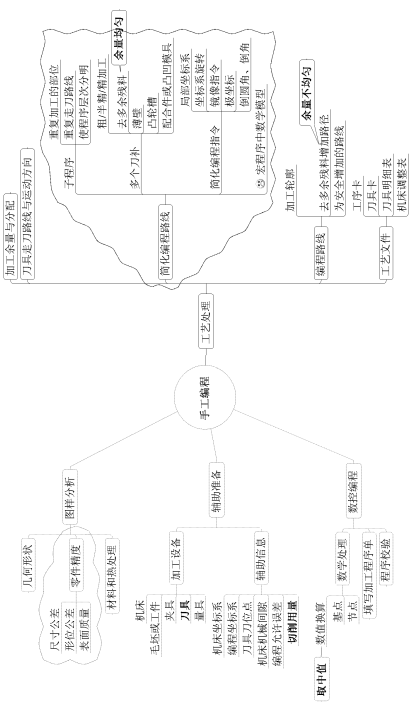
\includegraphics{images/tu1} 
	\caption{手工编程思维导图}\label{手工编程思维导图}
\end{figure}

\subsubsection{数控机床的操作}
如下面的思维导图 \ref{数控机床的操作思维导}
\begin{figure}	
	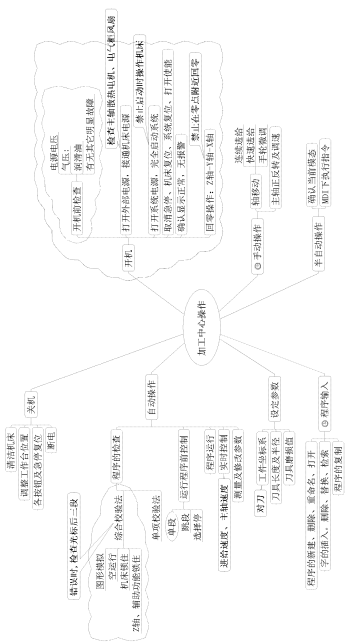
\includegraphics{images/tu2} 
	\caption{数控机床的操作思维导图} \label{数控机床的操作思维导}
\end{figure}

\subsubsection{数控机床指令}
\paragraph{G指令}\begin{itemize}
	\item G0 G1 G2 G3

	\item G17 G18 G19

	\item G9 G61 G62 G63 G64

	\item G4 \marginpar{说明介绍说明介绍说明介绍说明介绍说明介绍说明介绍}

	\item G20 G21

	\item G40 G41 G42 

	\item G43 G44 G49 \marginpar{说明介绍说明介绍说明介绍说明介绍说明介绍说明介绍}

	\item G90 G91

	\item G98 G99

	\item G81 G82 G83 G84 G85 G86 G87 G88 G89 G80 G73 G74 G76

\end{itemize}

\paragraph{M指令}

\begin{itemize}
	\item M0 M1 M2 M30

	\item M3 M4 M5 M19 

	\item M6 M7 M8 M9

	\item M98 M99

\end{itemize}

\paragraph{其它指令}
\subsubsection{常见加工结构}
\begin{itemize}
	\item 平面

	\item 外轮廓

	\item (岛屿)

	\item 孔
	\item 凸轮槽

	\item 复杂零件

	\item 配合零件

	\item CAD/CAM

	\item 宏程序

	\item 其它
\end{itemize}
\subsubsection{上学期期末试卷分析}
\subsection{课堂小结}
主要复习了数控方面的基本知识。
\vfill
\subsection{布置作业}
\begin{enumerate}[1、]
	\item 自选一零件图, 写出其工艺与程序;

	\item 写出如图所示零件的程序及与工艺;
\end{enumerate}
\vfill

\jxhj{%教学后记
	}
\skrq{%授课日期
	2017年2月27日 4-5节}
\ktmq{%课题名称
	变量编程概述 }
\jxmb{%教学目标,每行前面要加 \item
	\item 掌握变量的概念;

	\item 掌握变量的赋值于引用;

	\item 掌握表达式的使用;

	\item 会用变量编程;}
\jxzd{%教学重点,每行前面要加 \item
	\item 变量的概念;

	\item 表达式的使用;}
\jxnd{%教学难点,每行前面要加 \item
	\item 用变量编程;}
\jjff{%教学方法
	通过讲述、举例、演示法来说明;}

\makeshouye %制作教案首页

%%%%教学内容
\subsection{组织教学}
\begin{enumerate}[\hspace{2em}1、]
	\item 集中学生注意力;
	\item 清查学生人数;
	\item 维持课堂纪律;
\end{enumerate}
\subsection{复习导入及主要内容}
\begin{enumerate}[\hspace{2em}1、]
\item 复习;
\item 了解学生情况;
\end{enumerate}
\subsection{教学内容及过程}
\subsubsection{变量与常量} \marginpar{举例说明}
常量:指其值不变的量。如数值:1、4、6
\par
字符: “A”、“b”
\par
布尔值:“TURE”、“FALSE”
\par
变量:由变量名(变量号)和变量值组成,其值可以改变,

变量就是指其值可以改变的量。
\par
分析:程序结构相同,如果使用变量,则两个程序可以合为一个程序。
\par
长 宽 圆弧半径 深度等 都可以使用变量

可以用表达式来指定变量。
\subsubsection{Fanuc上的变量}
\begin{enumerate}[1、]
	\item 变量号(变量名)


\#1-\#33 

  \#100-\#199 
  
   \#500-\#999  
   
   \#1000以上


由变量符号“\#”和后面的变量号组成。
\item 变量的赋值:


赋值是指将一个数据赋予一个变量
\begin{enumerate}[(1)]
	\item 在程序中赋值:

\#1=10      \#2=5+5       \#3=\#3+1  \#5=\#7


注意: “=”为赋值号, 并等于号


赋值号“=”两内容不能随意互换, 左边只能是变量, 而右边可有是表达式, 数值或变量.


一个赋值语句只能给一个变量赋值.


可以多次给一个变量赋值, 新变量值将取代原变量值. 


赋值表达式的运算顺序与数学运算顺序相同


\item 在宏程序调用指令中赋值:(不讲)


如 G66 P5000 A10.0 B11.0


A10.0 B11.0 会给5000号宏程序中的\#1, \#2 赋值


宏调用中的A B C 与 \#1 \#2… \#20有一种邦定关系.


\item  在系统参数中设定变量的值:


Fanuc中操作如下: 


Offset-----[下一页]-------[Macro]


\#1--\#33   \#100--\#199   \#500--\#999


\end{enumerate}

\item 变量值的范围及小数点


定义变量时,整数值的小数点可以省略。

如:\# 100=123   变量\#100的值为123.000

\item 变量值的引用

在程序中使用变量时, 在相应的字后跟上变量号即可. 当用表达式指定变量时, 必须把表达式放在括号中, 如
:

G1 X\#\ 1 Y\#2


G1 X[-\#1-10] 


改变变量的符号, 可直接在\#前面加“-”, 如 G1 X-\#1


注意: O N G L P / 后不能使用变量.


程序的修改。
\end{enumerate}

\subsubsection{变量的分类} 
系统变量, 用于系统内部运算时各种数据的存储. \#1000以上,如刀具当前位置和补偿值等.


用户变量, 包括局部变量与公共变量, 用户可以单独使用, 系统作为处理资料的一部分.


局部变量: \#1-\#33 , 只能在宏程序中存储数据, 例如运算结果, 断电时,局部变量清除(初始值为空)


公共变量: \#100-\#199(数据断电清除)


\#500-\#999(数据断电时也不会清除)


公共变量在不同的宏程序中意义相同(即公共变量对于主程序和从这些主程序调用的每一个宏程序来说是公用的.)


举例说明:  个人的钱包   局部的


班上的班费   公共的


实例程序的修改:讲解

\subsubsection{算术} 

1. 加减乘除:
\\
\#i=\#j+\#k           \#i=\#j-\#k
\\
\#i=\#j*\#k           \#i=\#j/\#k
 \\
2.三角函数:
\\
\#i=SIN[\#j]          \#i=COS[\#j]
\\
\#i=ASIN[\#j]         \#i=ACOS[\#j]
\\
\#i=TAN[\#j]         \#i=ATAN[\#j]/[\#k] (可理解为对边/邻边)
\\
注意: 三角函数及反三角函数的数值均以度为单位来指定
\\
如90度30分应表示为90.5度
\\
3.开平方根,舍入,绝对值:
\\
\#i=SQRT[\#j]        \#i=ABS[\#j]
\\
\#i=ROUND[\#j]
\\
4.指数对数
\\
\#i=EXP[\#j]
\\
\#i=LN[\#j]
\\
5.取整
\\
上取整  \#i=FIX[\#j]
\\
下取整  \#i=FUP[\#j]
\subsubsection{运算顺序与括号}
\subsection{课堂小结}
\vfill
\subsection{布置作业}
\begin{enumerate}[1、]
	\item 自选一零件图, 写出其工艺与程序.
	\item 写出如图所示零件的程序及与工艺.
\end{enumerate}
\vfill
\jxhj{%教学后记
	}
\skrq{%授课日期
	2017年3月7日 4-5节}
\ktmq{%课题名称
	变量Z向分层}
\jxmb{%教学目标,每行前面要加 \item
	\item 掌握用循环来实现Z向分层;
	\item 掌握条件表达式的确定(加不加“=”);
	\item 掌握if then的使用;}
\jxzd{%教学重点,每行前面要加 \item
	\item 循环来实现Z向分层;
	\item 条件表达式的确定(加不加“=”)}
\jxnd{%教学难点,每行前面要加 \item
	\item 条件表达式的确定(加不加“=”)}
\jjff{%教学方法
	通过讲述、举例、演示法来说明;}

\makeshouye %制作教案首页

%%%%教学内容
\subsection{组织教学}
\begin{enumerate}[\hspace{2em}1、]
	\item 集中学生注意力;
	\item 清查学生人数;
	\item 维持课堂纪律;
\end{enumerate}
\subsection{复习导入及主要内容}
\begin{enumerate}[\hspace{2em}1、]
\item 变量与常量;
\item Fanuc上的变量;
\item 变量的分类;
\item 运算;
\item 运算顺序与括号
\end{enumerate}
\subsection{教学内容及过程}
\subsubsection{Z向分层} \marginpar{举例说明}
\paragraph{基本思路} 
以前 G91+子程序。

G90 深度用 变量,每个深度进行计算。

G91 次数用 变量,次数递增记数。

\paragraph{形成循环:}
\begin{verbatim}
#1=0
N10 
#1=#1+4
G90 G1 z-#1
……
If [#1lt12] goto10

#1=0
N10
#1=#1+1
G91 g1 z-4.0
……
If [#1lt3] goto10
\end{verbatim}
尽量用G90。

\paragraph{思考一}
如果初始值为4,侧程序怎么改

\begin{verbatim}
#1=4
N10 
G90 G1 z-#1
……
#1=#1+4
If [#1    12] goto10
\end{verbatim}

讨论分析:

用  LE 
 
结论:

\#1=\#1+4 放在执行之前,判断的量是当前位置值,当前值为终点是,应结束循环,条件判断用 GT 或 LT

\#4=\#4+4 放在执行之后,判断的量是下一个位置的值,下一点为终止值时,应走到终点后结束循环,条件判断应用GE或LE。


\paragraph{思考二}

当加工深度为13mm时怎么改程序。

方法一:等分每层加工 13/4=3.25mm

方法二:第一层加工1mm 其余12/4=3mm

\#1=2    \#1=\#1-3

注意初始值的更换。

方法三:每层4mm 最后一层1mm

怎么实现?

\#1=0  \#1=\#1-4  到了16?

\subsubsection{IF  Then 指令}

格式:  if [条件] THEN [指令]

功能: 条件成立时 执行 THEN 后的指令

条件不成立时,跳过后面的指令。

如 if [\#1GT13] THEN \#1=13

不适合判断的是下一个值,会干涉判断。


\subsubsection{Z向分层的应用}
\begin{verbatim}
#1=0
N10 
#1=#1+4
If [#1 GT 13] then #1=13
G90 G1 z-#1
……
If [#1lt13] goto10
写成while就是:
#1=0
While [#1 lt 13] DO1
#1=#1+4
If [#1 GT 13] then #1=13
G90 G1 z-#1
……
END1
\end{verbatim}

实例:深度13

\subsection{课堂小结}

\begin{enumerate}[1、]
	\item Z向分层
	\item IF Then
	\item 应用
\end{enumerate}

\vfill
\subsection{布置作业}
\begin{enumerate}[1、]
	\item 自选1个图进行Z向分层应用。 
\end{enumerate}
\vfill
\jxhj{%教学后记
	}
\skrq{%授课日期
	2017年3月14日 4-5节}
\ktmq{%课题名称
	椭圆编程 }
\jxmb{%教学目标,每行前面要加 \item
	\item 掌握用循环来实现Z向分层;
	\item 掌握椭圆的宏程序思路;
	\item 掌握椭圆的宏程序。 }
\jxzd{%教学重点,每行前面要加 \item
	\item 循环来实现Z向分层;
	\item 椭圆的宏程序思路。 }
\jxnd{%教学难点,每行前面要加 \item
	\item 椭圆的宏程序思路。 }
\jjff{%教学方法
	通过讲述、举例、演示法来说明;}

\makeshouye %制作教案首页

%%%%教学内容
\subsection{组织教学}
\begin{enumerate}[\hspace{2em}1、]
	\item 集中学生注意力;
	\item 清查学生人数;
	\item 维持课堂纪律;
\end{enumerate}
\subsection{复习导入及主要内容}
\begin{enumerate}[\hspace{2em}1、]
\item Z向分层;
\item IF THEN 指令;
\item Z向分层的应用;
\end{enumerate}
\subsection{教学内容及过程}
\subsubsection{非圆曲线的拟合加工} %\marginpar{举例说明}
 数控机床一般中能作直线插补和圆弧插补. 遇到工件轮廓是非圆曲线的零件时. 常用直线段或圆弧去逼近非圆曲线. 即拟合加工. 只要拟合误差在允许的范围内就行了.
 
 \paragraph{分段}
 等插补段法(求最小曲率半径Rmin, 求在允许插补误差时的弦长,求坐标)
 
 等插补误差法(以起点建立误差圆, 求该圆与曲线的公切线的斜率, 以起点作公切线的平行线, 计算坐标.)
 
 其它方法: (等角度)
 
\paragraph{用直线拟合}
 弦线, 割线, 切线
 \paragraph{圆弧逼近法}
 通过三点作圆(这三点是上面分段中的三个点)
 
 计算圆心
 
 计算坐标
 
\subsubsection{椭圆的数学模型}
\paragraph {参数方程}
 $$X=A*cos(a)$$
 $$Y=B*sin(a)$$
  使用角度控制
\paragraph{ 普通方程}
 $$ \frac{X^2}{A^2} + \frac{Y^2}{B^2} =1 $$
  可使用$X$控制, 常用于车床
\subsubsection{流程控制}
\subsubsection{椭圆的宏程序}
\begin{verbatim}
N100 #3=#3-1
G1 X[#1*COS[#3]] Y[#1*SIN[#3]]
IF [#1 GT -180] GOTO100
\end{verbatim}
\subsubsection{GOTO指令}
无条件转移。
 
\subsection{课堂小结}

\begin{enumerate}[1、]
	\item 非圆曲线的拟合加工;
	\item 椭圆的数学模型;
	\item 流程控制
	\item 椭圆的宏程序
\end{enumerate}

\vfill
\subsection{布置作业}
\begin{enumerate}[1、]
	\item 编写一个比较通用的外圆加工轮廓。。 
\end{enumerate}
\vfill
\jxhj{%教学后记
	}
\skrq{%授课日期
	}
\ktmq{%课题名称
	椭圆弧编程 }
\jxmb{%教学目标,每行前面要加 \item
	\item 掌握siemens上的变量;
	\item 掌握Siemens上的if goto 指令;
	\item 掌握 Siemens上 while endwhile 指令
	\item 会用if then对变量进行修正。 }
\jxzd{%教学重点,每行前面要加 \item
	\item Siemens上变量、if GOTO;
	\item 对变量进行修正。 }
\jxnd{%教学难点,每行前面要加 \item
	\item 对变量进行修正。 }
\jjff{%教学方法
	通过讲述、举例、演示法来说明;}

\makeshouye %制作教案首页

%%%%教学内容
\subsection{组织教学}
\begin{enumerate}[\hspace{2em}1、]
	\item 集中学生注意力;
	\item 清查学生人数;
	\item 维持课堂纪律;
\end{enumerate}
\subsection{复习导入及主要内容}
\begin{enumerate}[\hspace{2em}1、]
\item Z向分层;
\item IF THEN 指令;
\item Z向分层的应用;
\end{enumerate}


\subsection{教学内容及过程}


\subsubsection{相关内容}
\paragraph{变量}
Fanuc: $\#1-\#33 \#100-\#199  \#500-\#999 \#1000$ 以上

Seimens:$ R1-R299 $     开头的系统变量

赋值:Fanuc:$\#101=50$

Seimens: $\#100=50$

引用: Fanuc  $ X\#101   X[\#101*50]$

Siemens$ X=R101  X=R101*50$

\paragraph{运算}

加减乘除

三角函数  $Sin[] Sin() Cos[] cos() tan[] tan()$

单位:度

反三角函数:$ Asin[] Acos[] ATan[]/[]$

$Asin() Acos() Atan2( , )$

$ASin/ACOS $不能大于1
其他函数:

平方根:$SQRT[]  SQRT() $   为正

绝对值:$ABS[]   ABS()$

舍入: $  Round[]  Round() $ 四舍五入

指数:   $EXP[]  exp()   A×10m$

对数:   $LN[]   lN()    logeA$

取整:    上取整  $ Fix[]$ 无条件去小数

Siemens 去小数取整   $Trunc()$

下取整   $Fup[]$  进位取整   
            
\paragraph{条件表达式}
等于:     EQ      =
小于:     LT      <
大于       GT      >
不等于     NE      <>
小于等于   LE      <=
大于等于   GE      >=
\paragraph{流程控制}
A、无条件转移

Fanuc: \verb|GOTO____|

Siemens: GOTO/GOTOB/GOTOF  AA

B、有条件转移

Fanuc: if \[条件表达式\] GOTO

Siemens: IF  条件表达式  GOTO/GOTOB/GOTOF BB

C、循环

Fanuc:  while [条件表达式] DOm

ENDm    m只能为1、2、3

Siemens: while 条件

Endwhile 

\paragraph{值的修正}

Fanuc:  if[条件表达式]then

Siemens: if  条件

Endif

\subsubsection{椭圆弧加工}
参考程序:

零件图如图 \ref{椭圆弧加工} 所示:

	\begin{figure}
\centering	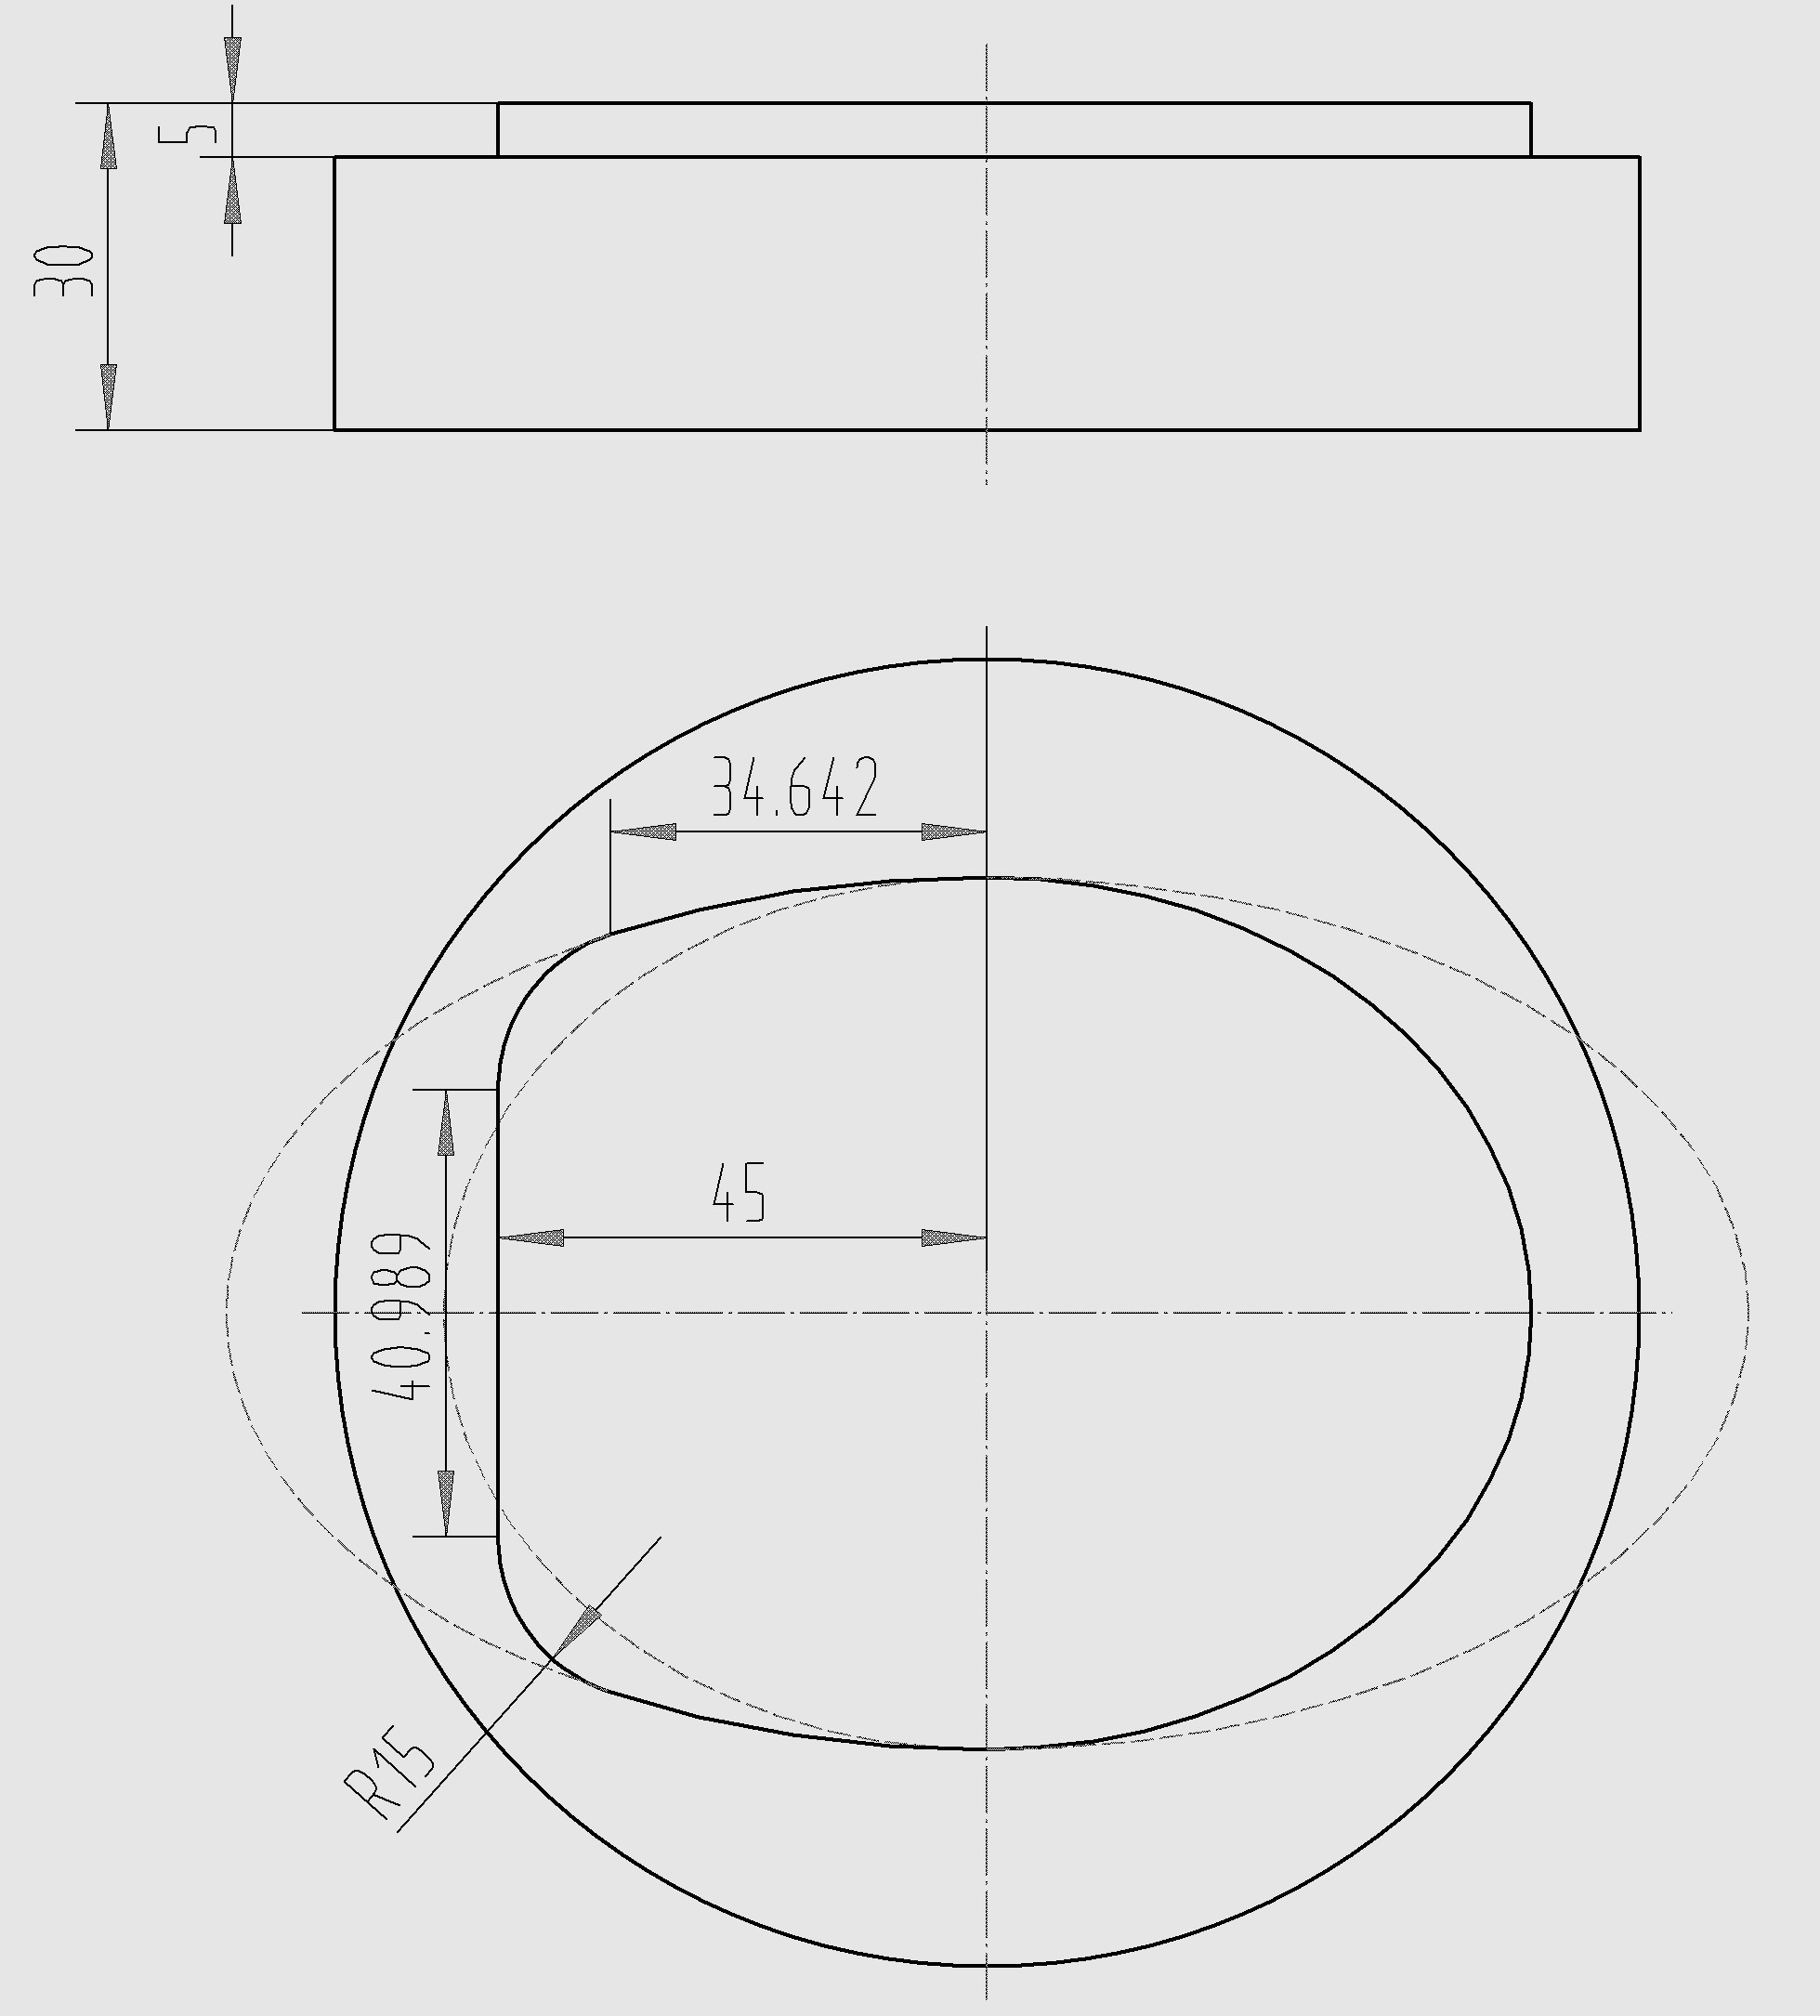
\includegraphics[width=0.8\textwidth]{images/5-1.jpg}
	\caption{椭圆弧加工} \label{椭圆弧加工}
\end{figure}


GX01 \\
G54G17G40G90G64\\
CFC\\
T1D1\\
M3S500\\
G1Z30.F2000\\
X-70.Y0\\
Z5.0\\
Z-5.0F200\\
G1G41X-60.0Y-15.D1\\
G3X-45.Y0R15.\\
G1Y20.495\\
R1=ACOS(-34.642/70)\\
R2=-R1\\
G2 X-34.642  Y=40*SIN(R1)  CR=15.\\
WHILE  R1 >90\\
R1=R1-1\\
G1 X=70*COS(R1)  Y=40*SIN(R1)\\
ENDWHILE\\
WHILE  R1>-90\\
R1=R1-1
G1 X=50*COS(R1)  Y=40*SIN(R1)\\
ENDWHILE\\
WHILE  R1>R2\\
R1=R1-1\\
G1 X=70*COS(R1)  Y=40*SIN(R1)\\
ENDWHILE\\
G2 X-45. Y20.495 R15.\\
G1 Y0\\
G3X-60.Y15.R15.\\
G1G40X-70.Y0\\
Z30.F2000\\
M5\\
M2\\

\subsubsection{应用实例}
正多边形加工思路

	\begin{figure}
	\centering	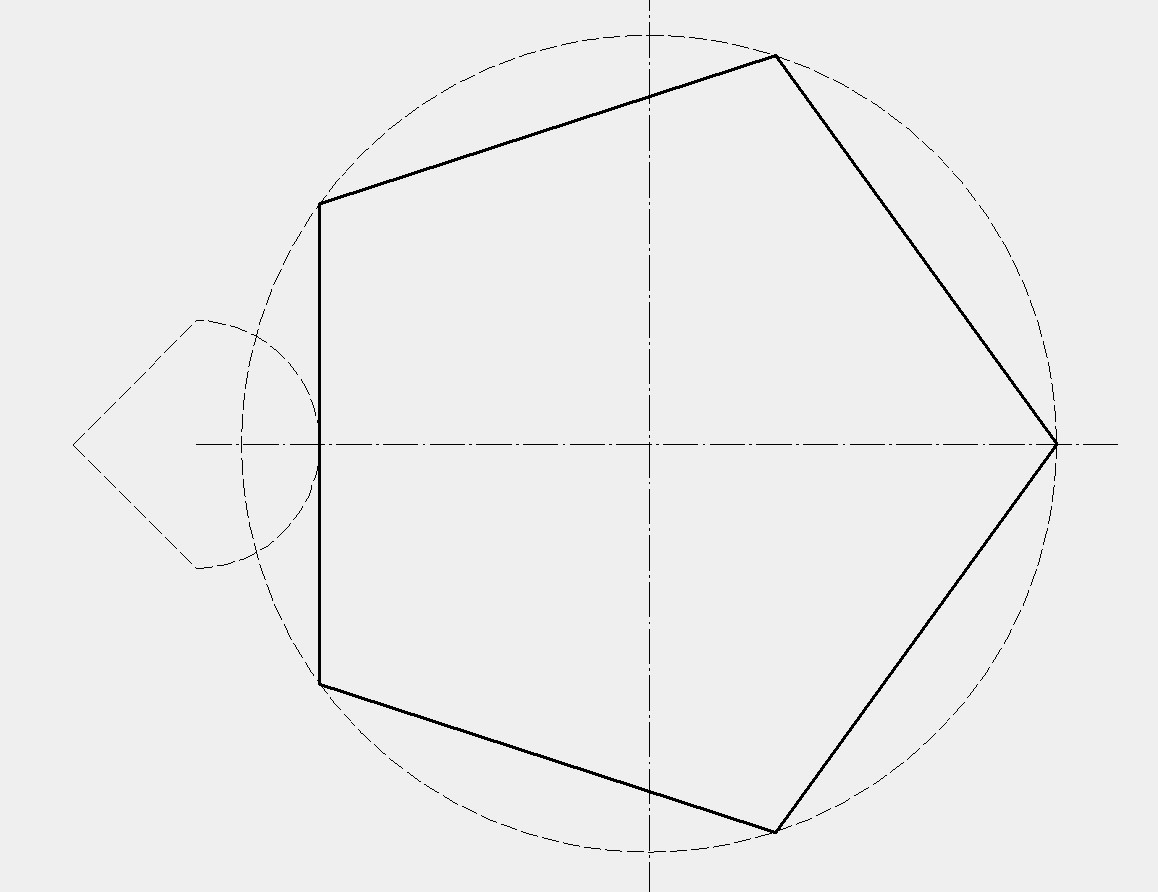
\includegraphics[width=0.8\textwidth]{images/5-2.jpg}
	\caption{正多边形加工} \label{正多边形加工}
\end{figure}

\subsection{课堂小结}
\begin{enumerate}[1、]
	\item 非圆曲线的拟合加工;
	\item 椭圆的数学模型;
	\item 流程控制
	\item 椭圆的宏程序
\end{enumerate}

\vfill
\subsection{布置作业}
\begin{enumerate}[1、]
	\item 编写一个比较通用的外圆加工轮廓。 
\end{enumerate}
\vfill
\jxhj{%教学后记
	}
\skrq{%授课日期
	}
\ktmq{%课题名称
	 局部坐标系}
\jxmb{%教学目标,每行前面要加 \item
	\item 掌握Fanuc上G52指令的格式;
	\item 掌握Siemens上Trans指令的格式;
	\item 掌握用局部坐标系指令编程。 }
\jxzd{%教学重点,每行前面要加 \item
	\item Fanuc上G52指令的格式;
	\item 用局部坐标系指令编程。 }
\jxnd{%教学难点,每行前面要加 \item
	\item 用局部坐标系指令编程。 }
\jjff{%教学方法
	通过讲述、举例、演示法来说明;}

\makeshouye %制作教案首页

%%%%教学内容
\subsection{组织教学}
\begin{enumerate}[\hspace{2em}1、]
	\item 集中学生注意力;
	\item 清查学生人数;
	\item 维持课堂纪律;
\end{enumerate}
\subsection{复习导入及主要内容}
\begin{enumerate}[\hspace{2em}1、]
\item 相关内容;
\item 椭圆弧加工;
\item 应用实例;
\end{enumerate}


\subsection{教学内容及过程}
\subsubsection{几种坐标系}
\paragraph{工件坐标系}
G54-G59、G92

G54-G59是在机床参数中以机床坐标为基准设定工件坐标系

G92是在程序中以刀具当前位置为基准设定工件坐标系

一般使用G54~G59指令后,就不再使用G92指令。

\paragraph{机床坐标系}
G53

当需要用机床坐标系编程时,用G53指令。

机床坐标系通过回零(回参考点)建立。

如坐标系不对,可通过回零重新建立机床坐标系,机床坐标系原点在机床上是固定的一个点,这个点不会变的。
\paragraph{局部坐标系}
G52、Trans

在工件坐标上建立一个子工件坐标系。即局部坐标系。
\subsubsection{Fanuc上局部坐标系}
指令格式:  G52 X\_ Y\_ Z\_;建立局部坐标系

G52 X0 Y0 Z0 ;取消局部坐标系。

说明:其X、Y的定义是原坐标系的程序原点到子坐标系的程序原点之向量值。

G52 X0 Y0;=>表示回复到原坐标系。

注意:
\begin{enumerate}[\hspace{2em}A、]
	\item 局部坐标系设定不改变工件和机床坐标系。 
\item 当用G50定义工件坐标系时,如果没有对局部坐标系中的所有轴指定坐标值,局部坐标系保持不变。
如果没有为局部坐标系中的任何轴指定坐标值,局部坐标系被取消。 
\item G52暂时取消刀尖半径补偿中的偏移。 
\item 在绝对方式紧跟G52之后指令一个运动指令。 
\item 复位时是否取消局部坐标系取决于参数的设定。当3402号参数的第6位(CLR)或者1202号参数3位(RLC)设为1时,局部坐标系在复位状态被取消。 
\item 手动返回参考点是否取消局部坐标系取决于ZCL的设定(参数1201的第2位)。
\end{enumerate}
\subsubsection{Siemens上的局部坐标系}
指令格式:

TRANS X\_ Y\_ Z\_ ;可编程的偏移,清除所有有关偏移、旋转、比例系数、镜像的指令 

ATRANS X\_ Y\_ Z\_ ;可编程的偏移,附加于当前的指令 

TRANS;不带数值清除所有有关偏移、旋转、比例系数、镜像的指令 

TRANS/ATRANS 指令要求一个独立的程序段。

\subsubsection{编程实例}
在数控机床上加工如图\ref{局部坐标系}所示的零件,完成工艺分析及加工程序的编写。

\begin{figure}
	\centering	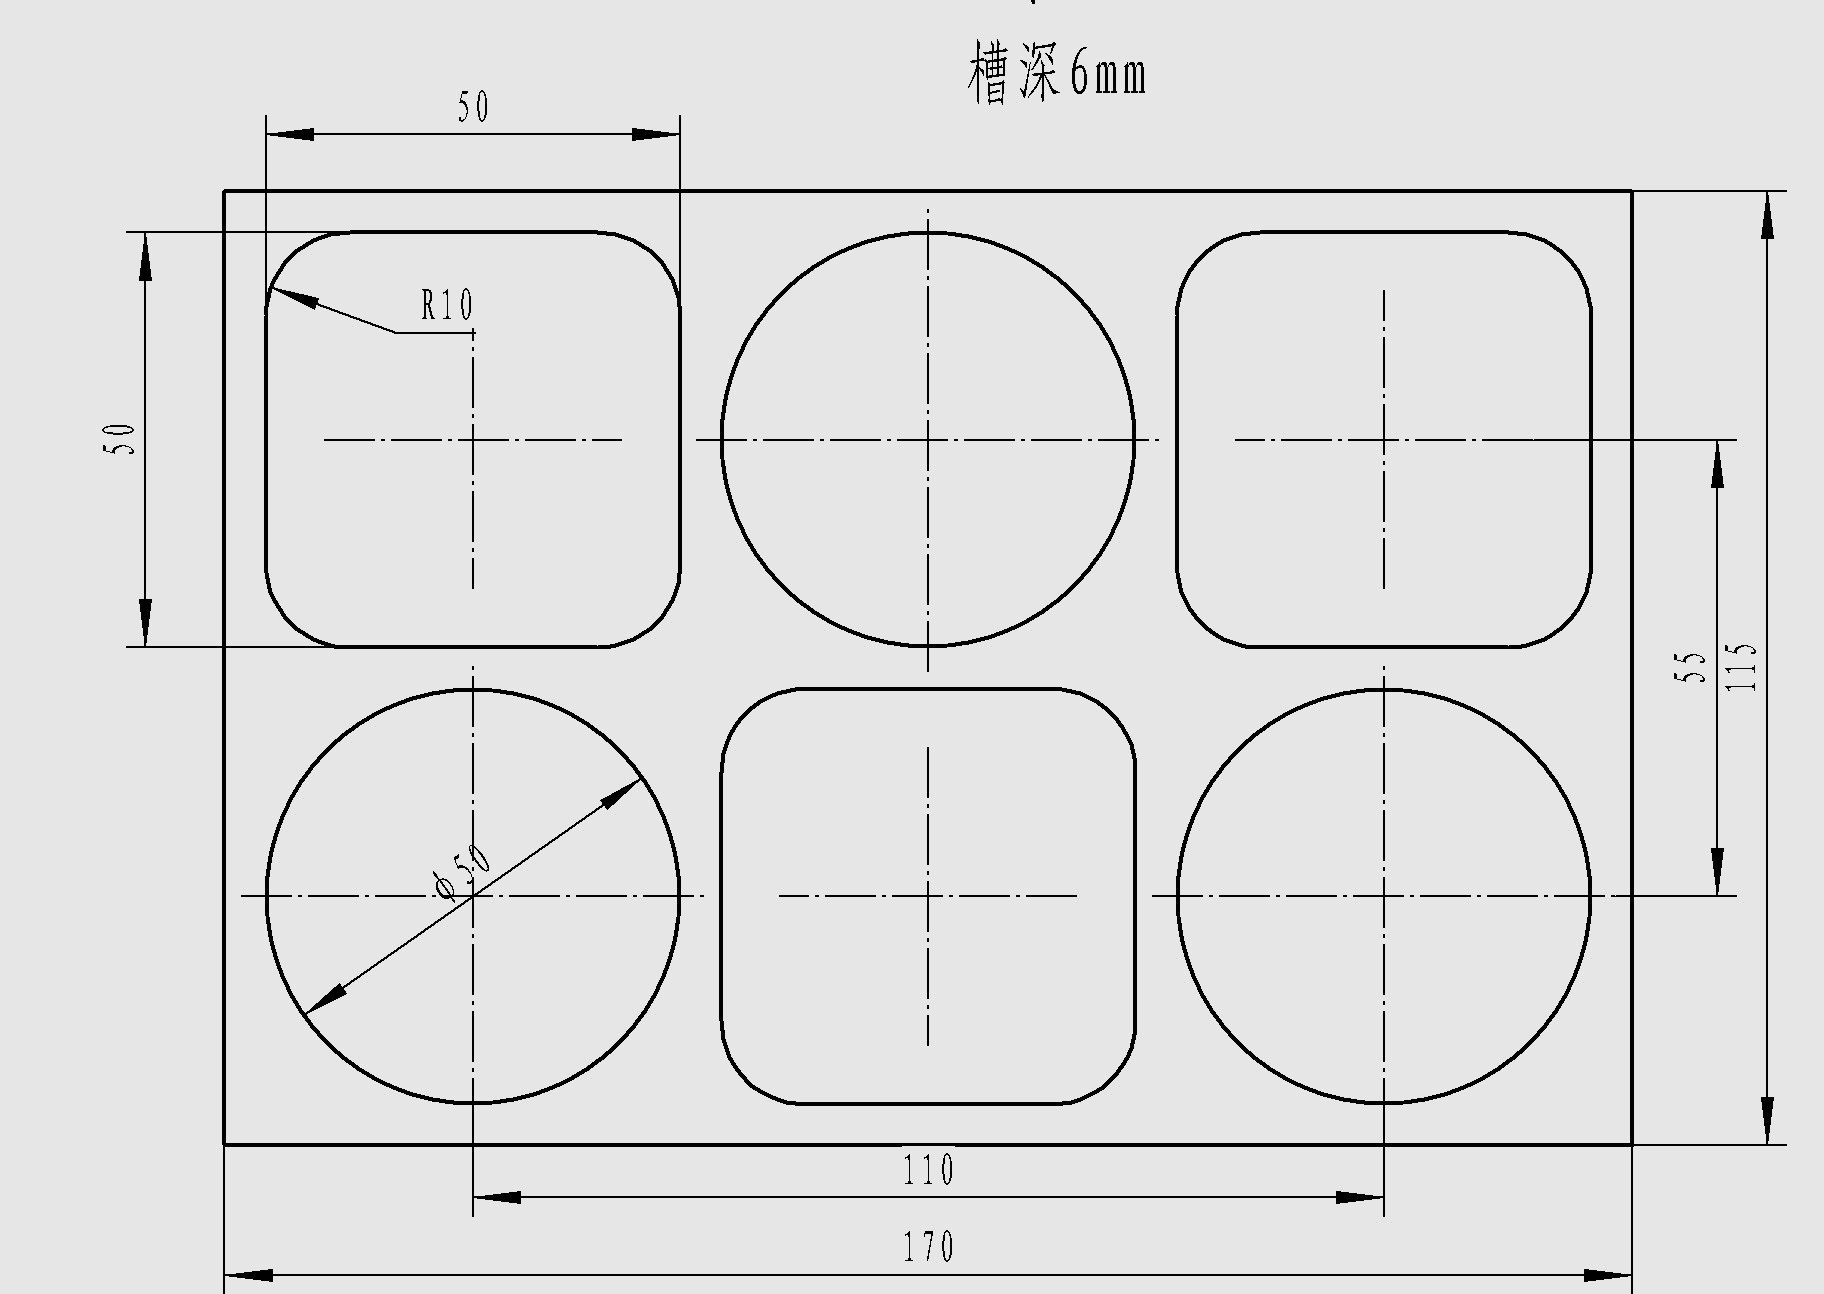
\includegraphics[width=0.8\textwidth]{images/6-1.jpg}
	\caption{局部坐标系} \label{局部坐标系}
\end{figure}

\paragraph{工件坐标系}
\paragraph{装夹}
\paragraph{刀具}
φ12立铣刀

φ8立铣刀
\paragraph{加工顺序}


\subsubsection{应用实例2}
如图\ref{局部坐标系2}所示,加工40*40矩形凸台,高3mm,刀具为Ф14的平底刀。
\begin{figure}
	\centering	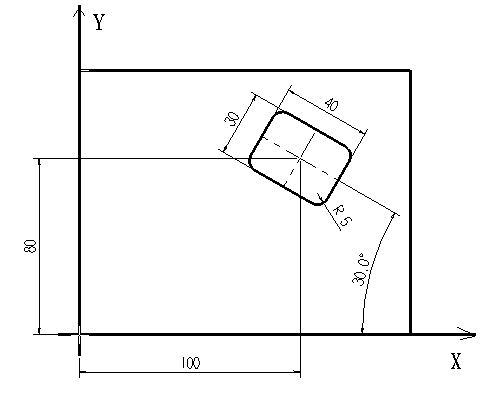
\includegraphics[width=0.8\textwidth]{images/6-2}
	\caption{局部坐标系2} \label{局部坐标系2}
\end{figure}

分析:
\begin{itemize}
\item 凸台为倾斜形式,可以使用旋转指令编程。
\item 凸台四角带圆角,可以使用倒圆角指令编程。
\item 使用局部坐标系,将当前工件坐标系移至凸台的中心处。
\end{itemize}
加工程序如下:
\begin{verbatim}
O1(FANUC)
G54G17G90G40
G01Z100F2000
M03S500
G52X100Y80 当前工件坐标系移至凸台的中心处
G68X0Y0R-30 当前工件坐标系顺时针旋转30度
G00X-35Y0
G01Z-3F1000            
G01G41X-30Y-10D01
G03X-20Y0R10
G01Y15,R5 倒圆角R5
X20,R5
Y-15,R5
X-20,R2
Y0
G03X-30Y10R10
G01G40X-35Y0
G01Z100F2000
G69 取消坐标系旋转
G52X0Y0 取消坐标系平移
M05
M30
\end{verbatim}



\subsection{课堂小结}
\begin{enumerate}[1、]
	\item 几种坐标系;
	\item Fanuc 上的局部坐标系;
	\item Siemens 上的局部坐标系;
	\item 编程实例。
\end{enumerate}

\vfill
\subsection{布置作业}
\begin{enumerate}[1、]
	\item 综合习题一。 
\end{enumerate}
\vfill
\jxhj{%教学后记
	}
\skrq{%授课日期
	2017年4月11日 4-5节}
\ktmq{%课题名称
	 坐标系旋转1}
\jxmb{%教学目标,每行前面要加 \item
	\item 掌握Fanuc上的坐标系旋转指令;
	\item 掌握Siemens上的坐标系旋转指令;
	\item 会使用旋转指令编程。 }
\jxzd{%教学重点,每行前面要加 \item
	\item Fanuc上的坐标系旋转指令;
	\item Siemens上的坐标系旋转指令。 }
\jxnd{%教学难点,每行前面要加 \item
	\item 使用旋转指令编程。 }
\jjff{%教学方法
	通过讲述、举例、演示法来说明;}

\makeshouye %制作教案首页

%%%%教学内容
\subsection{组织教学}
\begin{enumerate}[\hspace{2em}1、]
	\item 集中学生注意力;
	\item 清查学生人数;
	\item 维持课堂纪律;
\end{enumerate}
\subsection{复习导入及主要内容}
\begin{enumerate}[\hspace{2em}1、]
\item 几种坐标系;
\item Fanuc上的局部坐标系;
\item Siemens上的局部坐标系;
\item 应用实例;
\end{enumerate}


\subsection{教学内容及过程}

\subsubsection{旋转可用于以下几种情况}
\begin{itemize}
\item 编程轮廓与工件安装面成一定角度。
\item 有多个旋转的相同轮廓。
\item 同一轮廓上有多个旋转的要素。
\item 其它简化程序的地方。
\end{itemize}

\subsubsection{要素及原理}
\paragraph{旋转指令的要素}
\begin{itemize}
\item 旋转平面
\item 旋转中心
\item 旋转角度
\end{itemize}
\paragraph{原理}
在CNC内部对目标点进行转换(我们不用管它)
$$X’=X*COSA+Y*SINA$$
$$Y’=Y*COSA-X*SINA$$

上图中的A为-45度(即从$X------X’$的方向)
\subsubsection{Fanuc指令格式}
G17\\
G18 G68 α\_ β\_ R\_; 坐标系旋转开始\\
G19\\
:                  坐标系旋转模式 \\
:                  ( 坐标系被旋转 )\\
G69;                坐标系旋转取消模式\\
说明:\\
G17(G18或G19): 选择包含有被旋转图形的平面\\
α\_β\_ :         对应当前平面指令(G17,G18或G19)中的两个轴的绝对指令。\\
此指令指定了G68后面指定旋转中心的坐标。\\
R\_    :         正值为逆时针方向的角度位移。参数5400Bit0指定角度位移是绝对值位移或者由G码(G90或G91)来决定绝对值或相对值。\\
最小输入增量: 0.001度\\
有效数据范围: -360.000~360.000\\
注意事项:
\begin{enumerate}[A、]
	\item α\_β\_省略时,默认的旋转中心为刀具当前位置。
\item 程序的开头要加上G69安全注消指令。
\item 在坐标系旋转后,执行刀具半径补偿、刀具长度补偿、刀具偏置和其它补偿等,要在坐标系旋转取消前取消补偿。
\item 在坐标系旋转中,不得执行与坐标系有关的指令。如:G27、G28、G29、G30,G52-G59。
\item  坐标系旋转取消(G69)后的第一个指令必须用绝对值编程。用增量值则不能正确的执行。
\item 坐标系G68后的第一个指令应用绝对值编程,用增量值编程,则    会以刀具当前为中心进行第二次旋转,如图\ref{旋转}所示:
\begin{figure}
	\centering	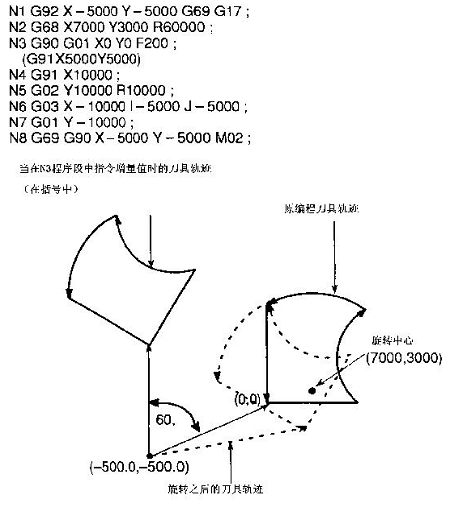
\includegraphics[width=0.8\textwidth]{images/7-1}
	\caption{旋转} \label{旋转}
\end{figure}
\item 有多个旋转时,旋转中的终点应与下一个旋转的启点重合。或者另外增加路径定位。
\end{enumerate}
\subsubsection{Sienes指令格式}
功能:在当前的平面G17或G18或G19中执行旋转,值为 RPL=\_,单位为度。\\
编程:    ROT RPL=\_  可编程旋转,删除以前的偏移,旋转,比例系数和镜像指令。\\
AROT RPL=\_; 可编程旋转,附加于当前的指令\\
ROT    没有设定值:删除以前的偏移,旋转,比例系数和镜象\\
ROT/AROT指令要求一个独立的程序段。

注意:旋转中心始终在工件坐标系原点\\
工件坐标系原点可以通过TRANS X\_ Y\_ 进行平移。\\

\subsubsection{加工实例}
在数控机床上加工如图\ref{坐标系旋转}所示的零件,完成加工工艺及加工程序的编写:
\begin{figure}
	\centering	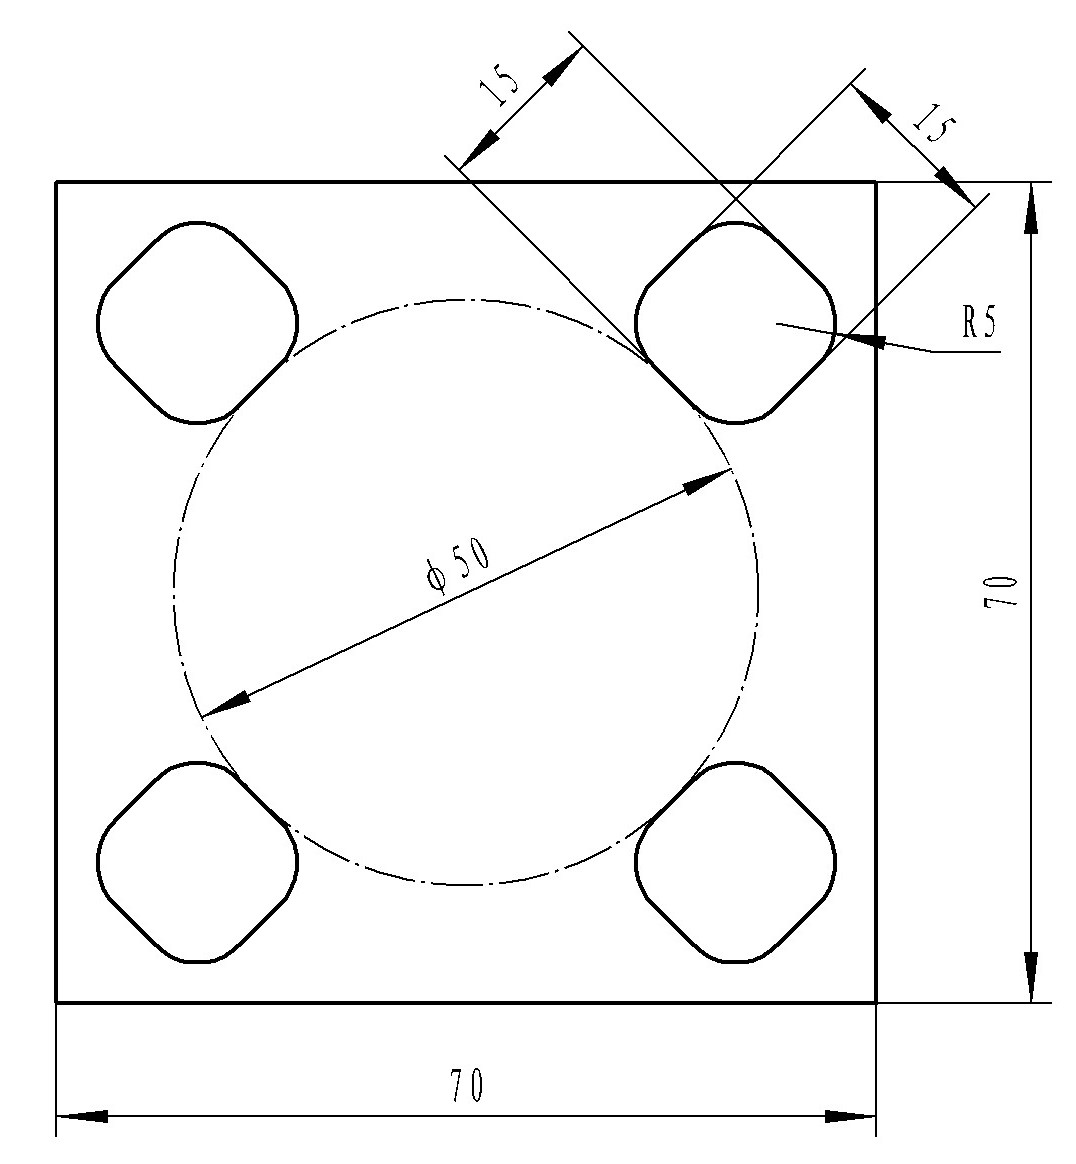
\includegraphics[width=0.8\textwidth]{images/7-2.jpg}
	\caption{坐标系旋转} \label{坐标系旋转}
\end{figure}
参考程序:

\begin{verbatim}
02
G54G17G40G49G90
M3S500
G43H1G1Z100.F2000;
G1X40.Y40.
Z5.0
Z0F2000
G68X0Y0R45.
M98P221
G69
\end{verbatim}


\subsection{课堂小结}
\begin{enumerate}[1、]
	\item 旋转可应用场合;
	\item 要素及原理;
	\item Fanuc旋转指令格式;
	\item Sienes旋转指令格式;
	\item 编程实例。
\end{enumerate}

\vfill
\subsection{布置作业}
\begin{enumerate}[1、]
	\item 综合习题一。 
\end{enumerate}
\vfill
\jxhj{%教学后记
	}
\skrq{%授课日期
	2017年4月18日 4-5节}
\ktmq{%课题名称
	 坐标系旋转2}
\jxmb{%教学目标,每行前面要加 \item
	\item 掌握Fanuc上的坐标系旋转指令;
	\item 掌握Siemens上的坐标系旋转指令;
	\item 会使用旋转指令编程。 }
\jxzd{%教学重点,每行前面要加 \item
	\item Fanuc上的坐标系旋转指令;
	\item Siemens上的坐标系旋转指令。 }
\jxnd{%教学难点,每行前面要加 \item
	\item 使用旋转指令编程。 }
\jjff{%教学方法
	通过讲述、举例、演示法来说明;}

\makeshouye %制作教案首页

%%%%教学内容
\subsection{组织教学}
\begin{enumerate}[\hspace{2em}1、]
	\item 集中学生注意力;
	\item 清查学生人数;
	\item 维持课堂纪律;
\end{enumerate}
\subsection{复习导入及主要内容}
\begin{enumerate}[\hspace{2em}1、]
\item 几种坐标系;
\item Fanuc上的局部坐标系;
\item Siemens上的局部坐标系;
\item 应用实例;
\end{enumerate}


\subsection{教学内容及过程}

\subsubsection{旋转可用于以下几种情况}
\begin{itemize}
\item 编程轮廓与工件安装面成一定角度。
\item 有多个旋转的相同轮廓。
\item 同一轮廓上有多个旋转的要素。
\item 其它简化程序的地方。
\end{itemize}

\subsubsection{要素及原理}
\paragraph{旋转指令的要素}
\begin{itemize}
\item 旋转平面
\item 旋转中心
\item 旋转角度
\end{itemize}
\paragraph{原理}
在CNC内部对目标点进行转换(我们不用管它)
$$X’=X*COSA+Y*SINA$$
$$Y’=Y*COSA-X*SINA$$

上图中的A为-45度(即从$X------X’$的方向)
\subsubsection{Fanuc指令格式}
G17\\
G18 G68 α\_ β\_ R\_; 坐标系旋转开始\\
G19\\
:                  坐标系旋转模式 \\
:                  ( 坐标系被旋转 )\\
G69;                坐标系旋转取消模式\\
说明:\\
G17(G18或G19): 选择包含有被旋转图形的平面\\
α\_β\_ :         对应当前平面指令(G17,G18或G19)中的两个轴的绝对指令。\\
此指令指定了G68后面指定旋转中心的坐标。\\
R\_    :         正值为逆时针方向的角度位移。参数5400Bit0指定角度位移是绝对值位移或者由G码(G90或G91)来决定绝对值或相对值。\\
最小输入增量: 0.001度\\
有效数据范围: -360.000~360.000\\
注意事项:
\begin{enumerate}[A、]
	\item α\_β\_省略时,默认的旋转中心为刀具当前位置。
\item 程序的开头要加上G69安全注消指令。
\item 在坐标系旋转后,执行刀具半径补偿、刀具长度补偿、刀具偏置和其它补偿等,要在坐标系旋转取消前取消补偿。
\item 在坐标系旋转中,不得执行与坐标系有关的指令。如:G27、G28、G29、G30,G52-G59。
\item  坐标系旋转取消(G69)后的第一个指令必须用绝对值编程。用增量值则不能正确的执行。
\item 坐标系G68后的第一个指令应用绝对值编程,用增量值编程,则    会以刀具当前为中心进行第二次旋转,如图\ref{旋转5}所示:
\begin{figure}
	\centering	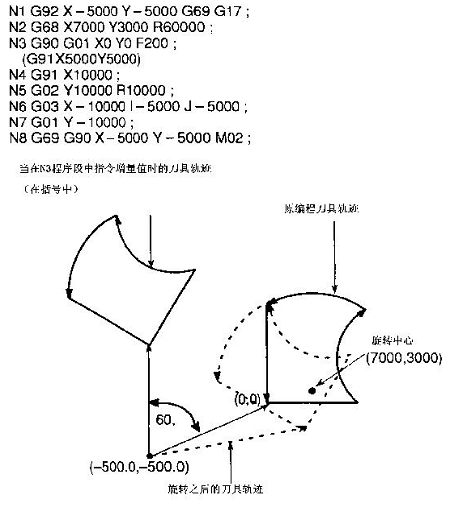
\includegraphics[width=0.8\textwidth]{images/7-1}
	\caption{旋转5} \label{旋转5}
\end{figure}
\item 有多个旋转时,旋转中的终点应与下一个旋转的启点重合。或者另外增加路径定位。
\end{enumerate}
\subsubsection{Sienes指令格式}
功能:在当前的平面G17或G18或G19中执行旋转,值为 RPL=\_,单位为度。\\
编程:    ROT RPL=\_  可编程旋转,删除以前的偏移,旋转,比例系数和镜像指令。\\
AROT RPL=\_; 可编程旋转,附加于当前的指令\\
ROT    没有设定值:删除以前的偏移,旋转,比例系数和镜象\\
ROT/AROT指令要求一个独立的程序段。

注意:旋转中心始终在工件坐标系原点\\
工件坐标系原点可以通过TRANS X\_ Y\_ 进行平移。\\

\subsubsection{加工实例}
在数控机床上加工如图\ref{坐标系旋转3}所示的零件,完成加工工艺及加工程序的编写:
\begin{figure}
	\centering	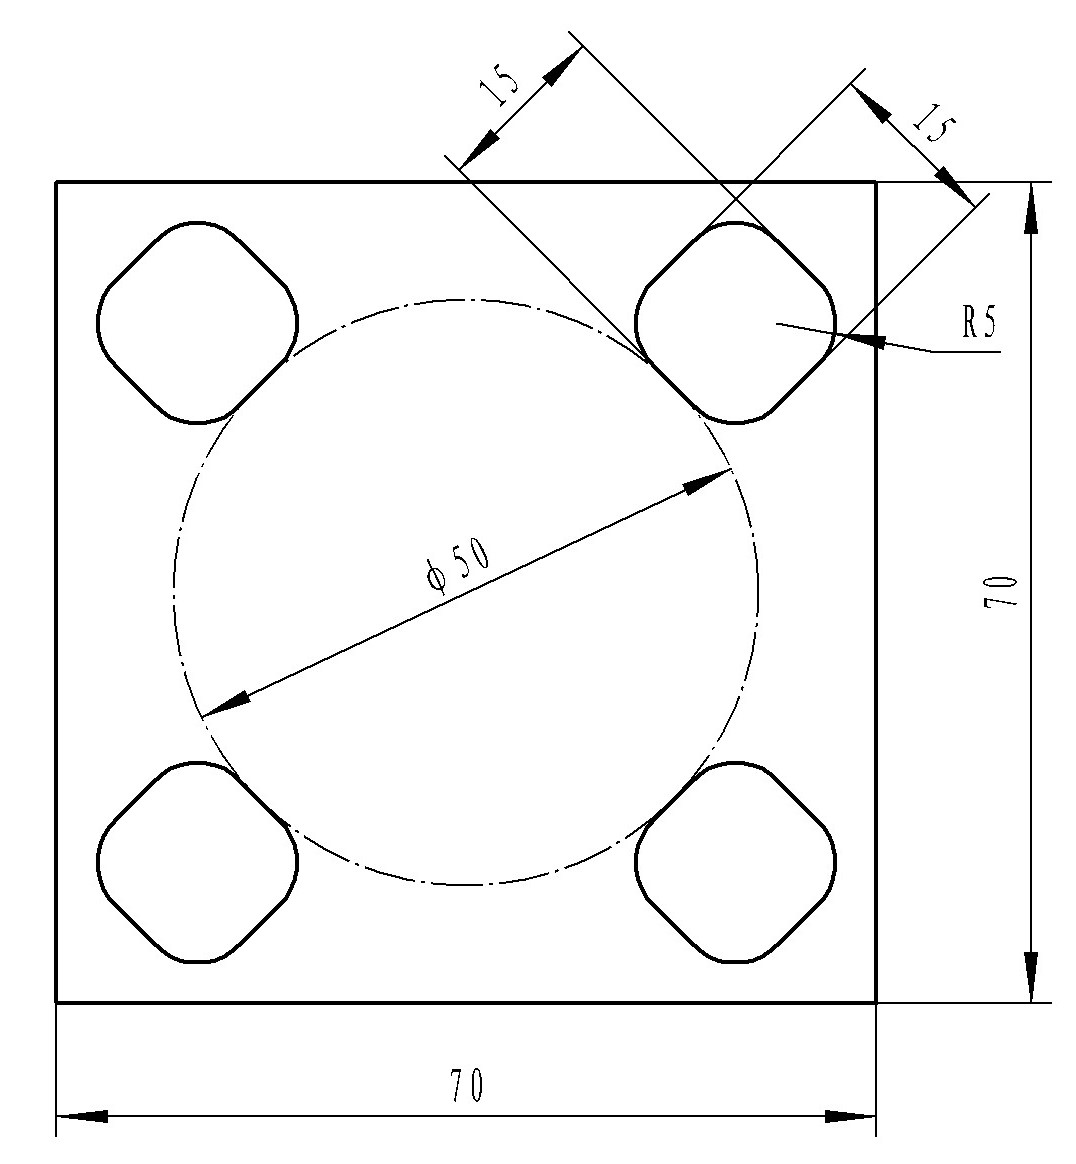
\includegraphics[width=0.8\textwidth]{images/7-2.jpg}
	\caption{坐标系旋转3} \label{坐标系旋转3}
\end{figure}
参考程序:

\begin{verbatim}
02
G54G17G40G49G90
M3S500
G43H1G1Z100.F2000;
G1X40.Y40.
Z5.0
Z0F2000
G68X0Y0R45.
M98P221
G69
\end{verbatim}


\subsection{课堂小结}
\begin{enumerate}[1、]
	\item 旋转可应用场合;
	\item 要素及原理;
	\item Fanuc旋转指令格式;
	\item Sienes旋转指令格式;
	\item 编程实例。
\end{enumerate}

\vfill
\subsection{布置作业}
\begin{enumerate}[1、]
	\item 综合习题一。 
\end{enumerate}
\vfill
\jxhj{%教学后记
	}
\skrq{%授课日期
	2017年4月24日 4-5节}
\ktmq{%课题名称
	 极坐标指令}
\jxmb{%教学目标,每行前面要加 \item
	\item 掌握Fanuc上极坐标指令的使用;
	\item 掌握Siemens上极坐标指令的使用;
	\item 灵活使用极坐标指令进行编程;
	\item 掌握加工工艺的分析。 }
\jxzd{%教学重点,每行前面要加 \item
	\item 极坐标知识和其指令的使用;
	\item 对加工轮廓进行处理后再编程。 }
\jxnd{%教学难点,每行前面要加 \item
	\item 加工轮廓进行处理后再编程。 }
\jjff{%教学方法
	通过讲述、举例、演示法来说明;}

\makeshouye %制作教案首页

%%%%教学内容
\subsection{组织教学}
\begin{enumerate}[\hspace{2em}1、]
	\item 集中学生注意力;
	\item 清查学生人数;
	\item 维持课堂纪律;
\end{enumerate}
\subsection{复习导入及主要内容}
\begin{enumerate}[1、]
	\item 旋转可应用场合;
	\item 要素及原理;
	\item Fanuc旋转指令格式;
	\item Sienes旋转指令格式;
	\item 编程实例。
\end{enumerate}



\subsection{教学内容及过程}

\subsubsection{加工轮廓的处理}
\begin{figure}[!hbtp]
	\centering	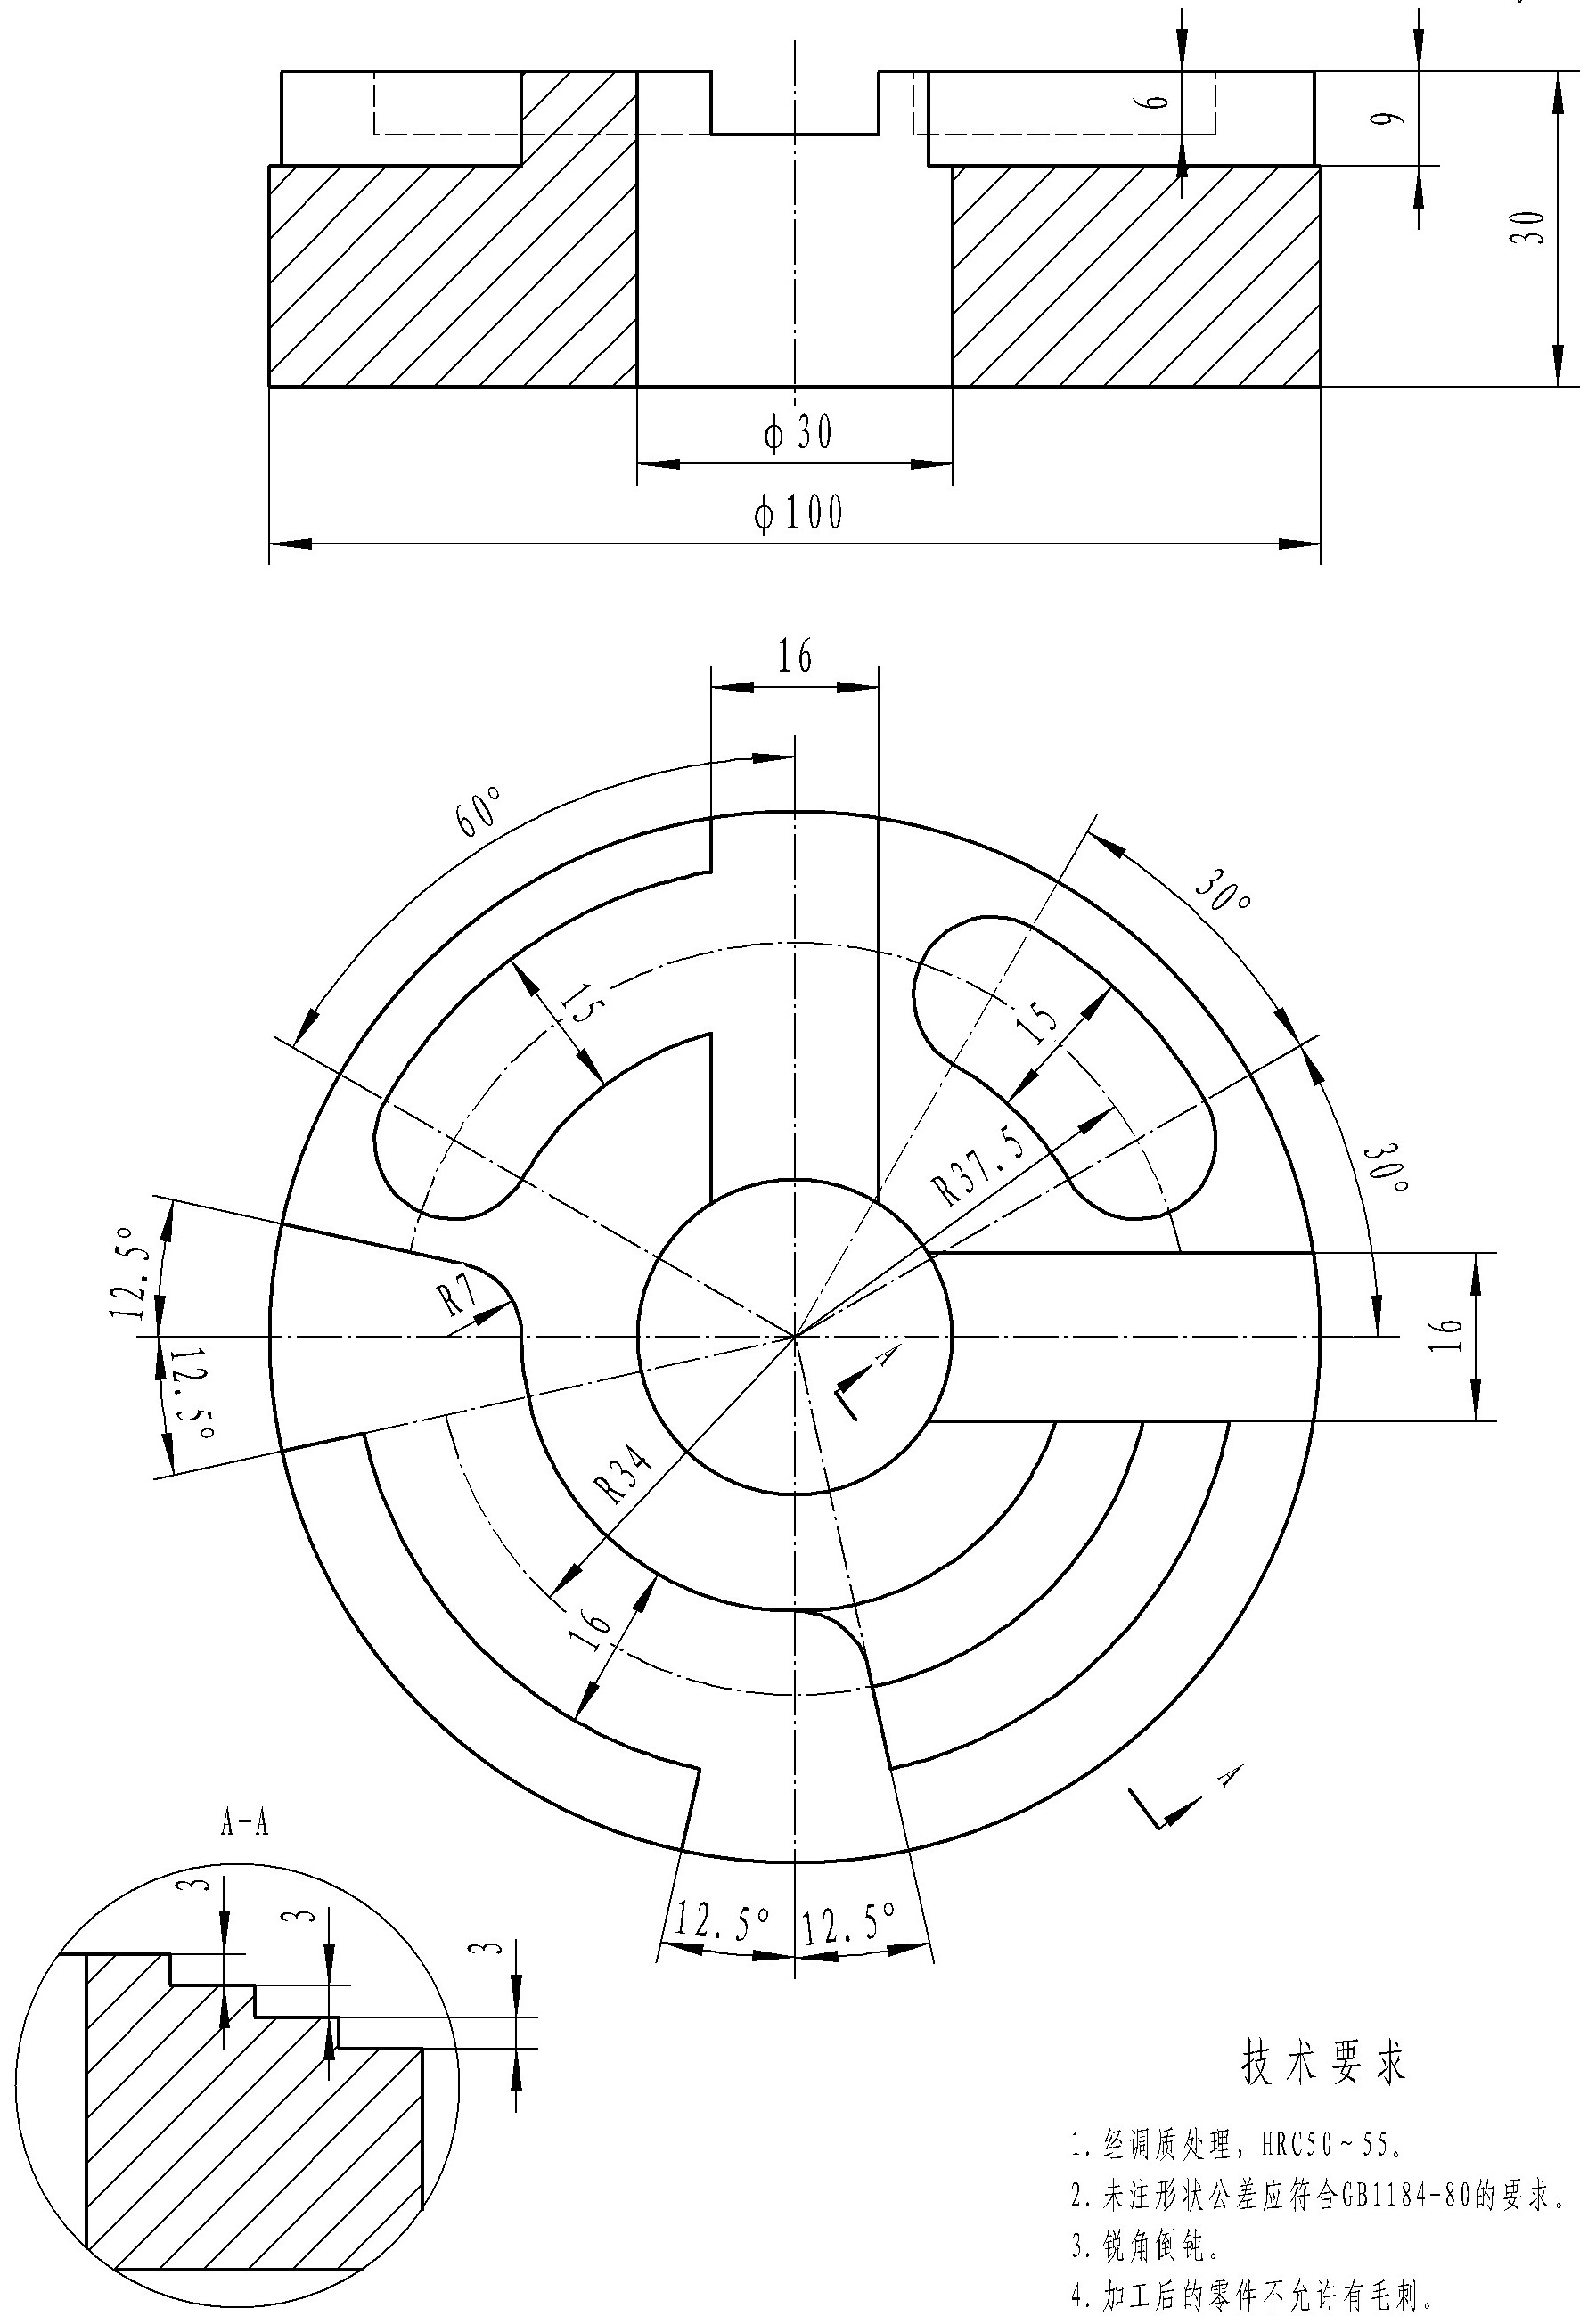
\includegraphics[width=0.8\textwidth]{images/9-1}
	\caption{极坐标实例} \label{极坐标实例}
\end{figure}
\textbf{加工轮廓的处理(改路径,延长)}
\paragraph{把加工轮廓进行拆分}
\noindent A、两个直槽:\\
标点的坐标,直角坐标(开放的)\\
B、小圆弧槽:\\
标点的坐标,使用极坐标\\
C、腰形槽:\\
标点的坐标,极坐标\\
D、扇形台阶\\
标点的坐标,极坐标\\
起点与终点不重合\\
编程时的处理\\
E、带翅膀的圆弧槽。
\paragraph{极坐标与 直角坐标的互换}
$$X=P*cosA$$
$$Y=P*sinA$$
$$P=X2+Y2$$
$$A=aictanY/X$$
\subsubsection{极坐标}
\paragraph{Fanuc上的极坐标}
指令格式: G\_\_ G~~ G16;启动极坐标指令(极坐标方式)\\
G~~ IP\_\_; 极坐标指令\\
:\\
G15;取消极坐标\\
说明:G\_\_极坐标指令的平面选择(G17、G18、G19)\\
G~~ G90指定工件坐标系的零点作为极坐标系原点,\\
G91指定当前位置作为极坐标系的原点。\\
IP\_\_指定极坐标系选择平面的轴地址及其值。\\
第1轴:极坐标半径\\
第2轴:极坐标角度 \\
用G90指定半径,极点设在工件坐标系原点。\\
如再用G90指定角度,角度是与X轴的夹角\\
如再用G91指定角度,角度是与当前位置的夹角\\
用G91指定半径,极点设在刀具当前位置。\\
如再用G90指定角度,角度是与X轴的夹角\\
如再用G91指定角度,角度是与当前位置的夹角。\\
限制:A、在极坐标方式中,对圆弧插补或螺旋线插补(G02,G03)用R 指定半径。\\
在极坐标方式中,不能用以下指令:\\
G4、G10、G52、G92、G53、G68、G51\\
在极坐标方式中不能倒角和倒圆\\
\paragraph{Siemens上的极坐标}
\textbf{极坐标,极点定义}:G110,G111,G112 \\
A、在直角坐标系中定义极点:\\
G110/G111/G112 X\_\_ Y\_\_ Z\_\_\\
B、在极坐标系中定义极点:\\
G110/G111/G112 AP=\_\_RP=\_\_\\
说明: \\
G110:相对于刀具最近到达的点(刀具当前位置)定义极点\\
G111:相对于当前工件坐标系定义极点\\
G112:相对于上一个有效极点定义极点\\
\textbf{在极坐标系中使用极坐标}\\
A、G0 AP=\_\_ RP=\_\_\\
B、G1 AP=\_\_ RP=\_\_\\
C、G2 AP=\_\_RP=\_\_\\
D、G3 AP=\_\_ RP=\_\_
说明:\\
AP=\_\_:极角,极点和目标点之间连线与角度参考方向之间的夹角(第一次角度参考方向线中一条),取值范围±(0-360),当用绝对坐标编程时,角度为相对于加工平面的水平轴方向,当用相对坐标编程时,上一个被编程角度作为参考位置。极角一直保持到新的极角被定义或工件坐标系被改变。\\
RP=\_\_:极半径,极点和目标点之间的距离,极半径一保持到新的极半径被定义。\\
所有与极坐标有关的输入必须在单个程序段内编程。用极坐标所定义的位置都可以用G0 G1 G2 G3去移动,极坐系在由G17/G18/G19所定义的加工平面内都有效。如果没有极坐标在使用,有效的工件坐标系的原点有用,\\
\subsubsection{加工工序} \marginpar{ 比较分析讲解}
A、铣上表面\\
B、铣ф30通孔(也可钻、扩、镗)\\
C、铣直槽和圆弧\\
……
由学生自己分析。\\


















\subsection{课堂小结}
\begin{enumerate}[1、]
	\item 加工轮廓的处理;
	\item 极坐标;
	\item 加工工序。
\end{enumerate}

\vfill
\subsection{布置作业}
\begin{enumerate}[1、]
	\item 自选一零件图, 写出其工艺与程序。 
\end{enumerate}
\vfill
\jxhj{%教学后记
	}
\skrq{%授课日期
	2017年5月1日 4-5节}
\ktmq{%课题名称
	 极坐标指令}
\jxmb{%教学目标,每行前面要加 \item
	\item 掌握Fanuc上极坐标指令的使用;
	\item 掌握Siemens上极坐标指令的使用;
	\item 灵活使用极坐标指令进行编程;
	\item 掌握加工工艺的分析。 }
\jxzd{%教学重点,每行前面要加 \item
	\item 极坐标知识和其指令的使用;
	\item 对加工轮廓进行处理后再编程。 }
\jxnd{%教学难点,每行前面要加 \item
	\item 加工轮廓进行处理后再编程。 }
\jjff{%教学方法
	通过讲述、举例、演示法来说明;}

\makeshouye %制作教案首页

%%%%教学内容
\subsection{组织教学}
\begin{enumerate}[\hspace{2em}1、]
	\item 集中学生注意力;
	\item 清查学生人数;
	\item 维持课堂纪律;
\end{enumerate}
\subsection{复习导入及主要内容}
\begin{enumerate}[1、]
	\item 旋转可应用场合;
	\item 要素及原理;
	\item Fanuc旋转指令格式;
	\item Sienes旋转指令格式;
	\item 编程实例。
\end{enumerate}



\subsection{教学内容及过程}

\subsubsection{加工轮廓的处理}
\begin{figure}[!hbtp]
	\centering	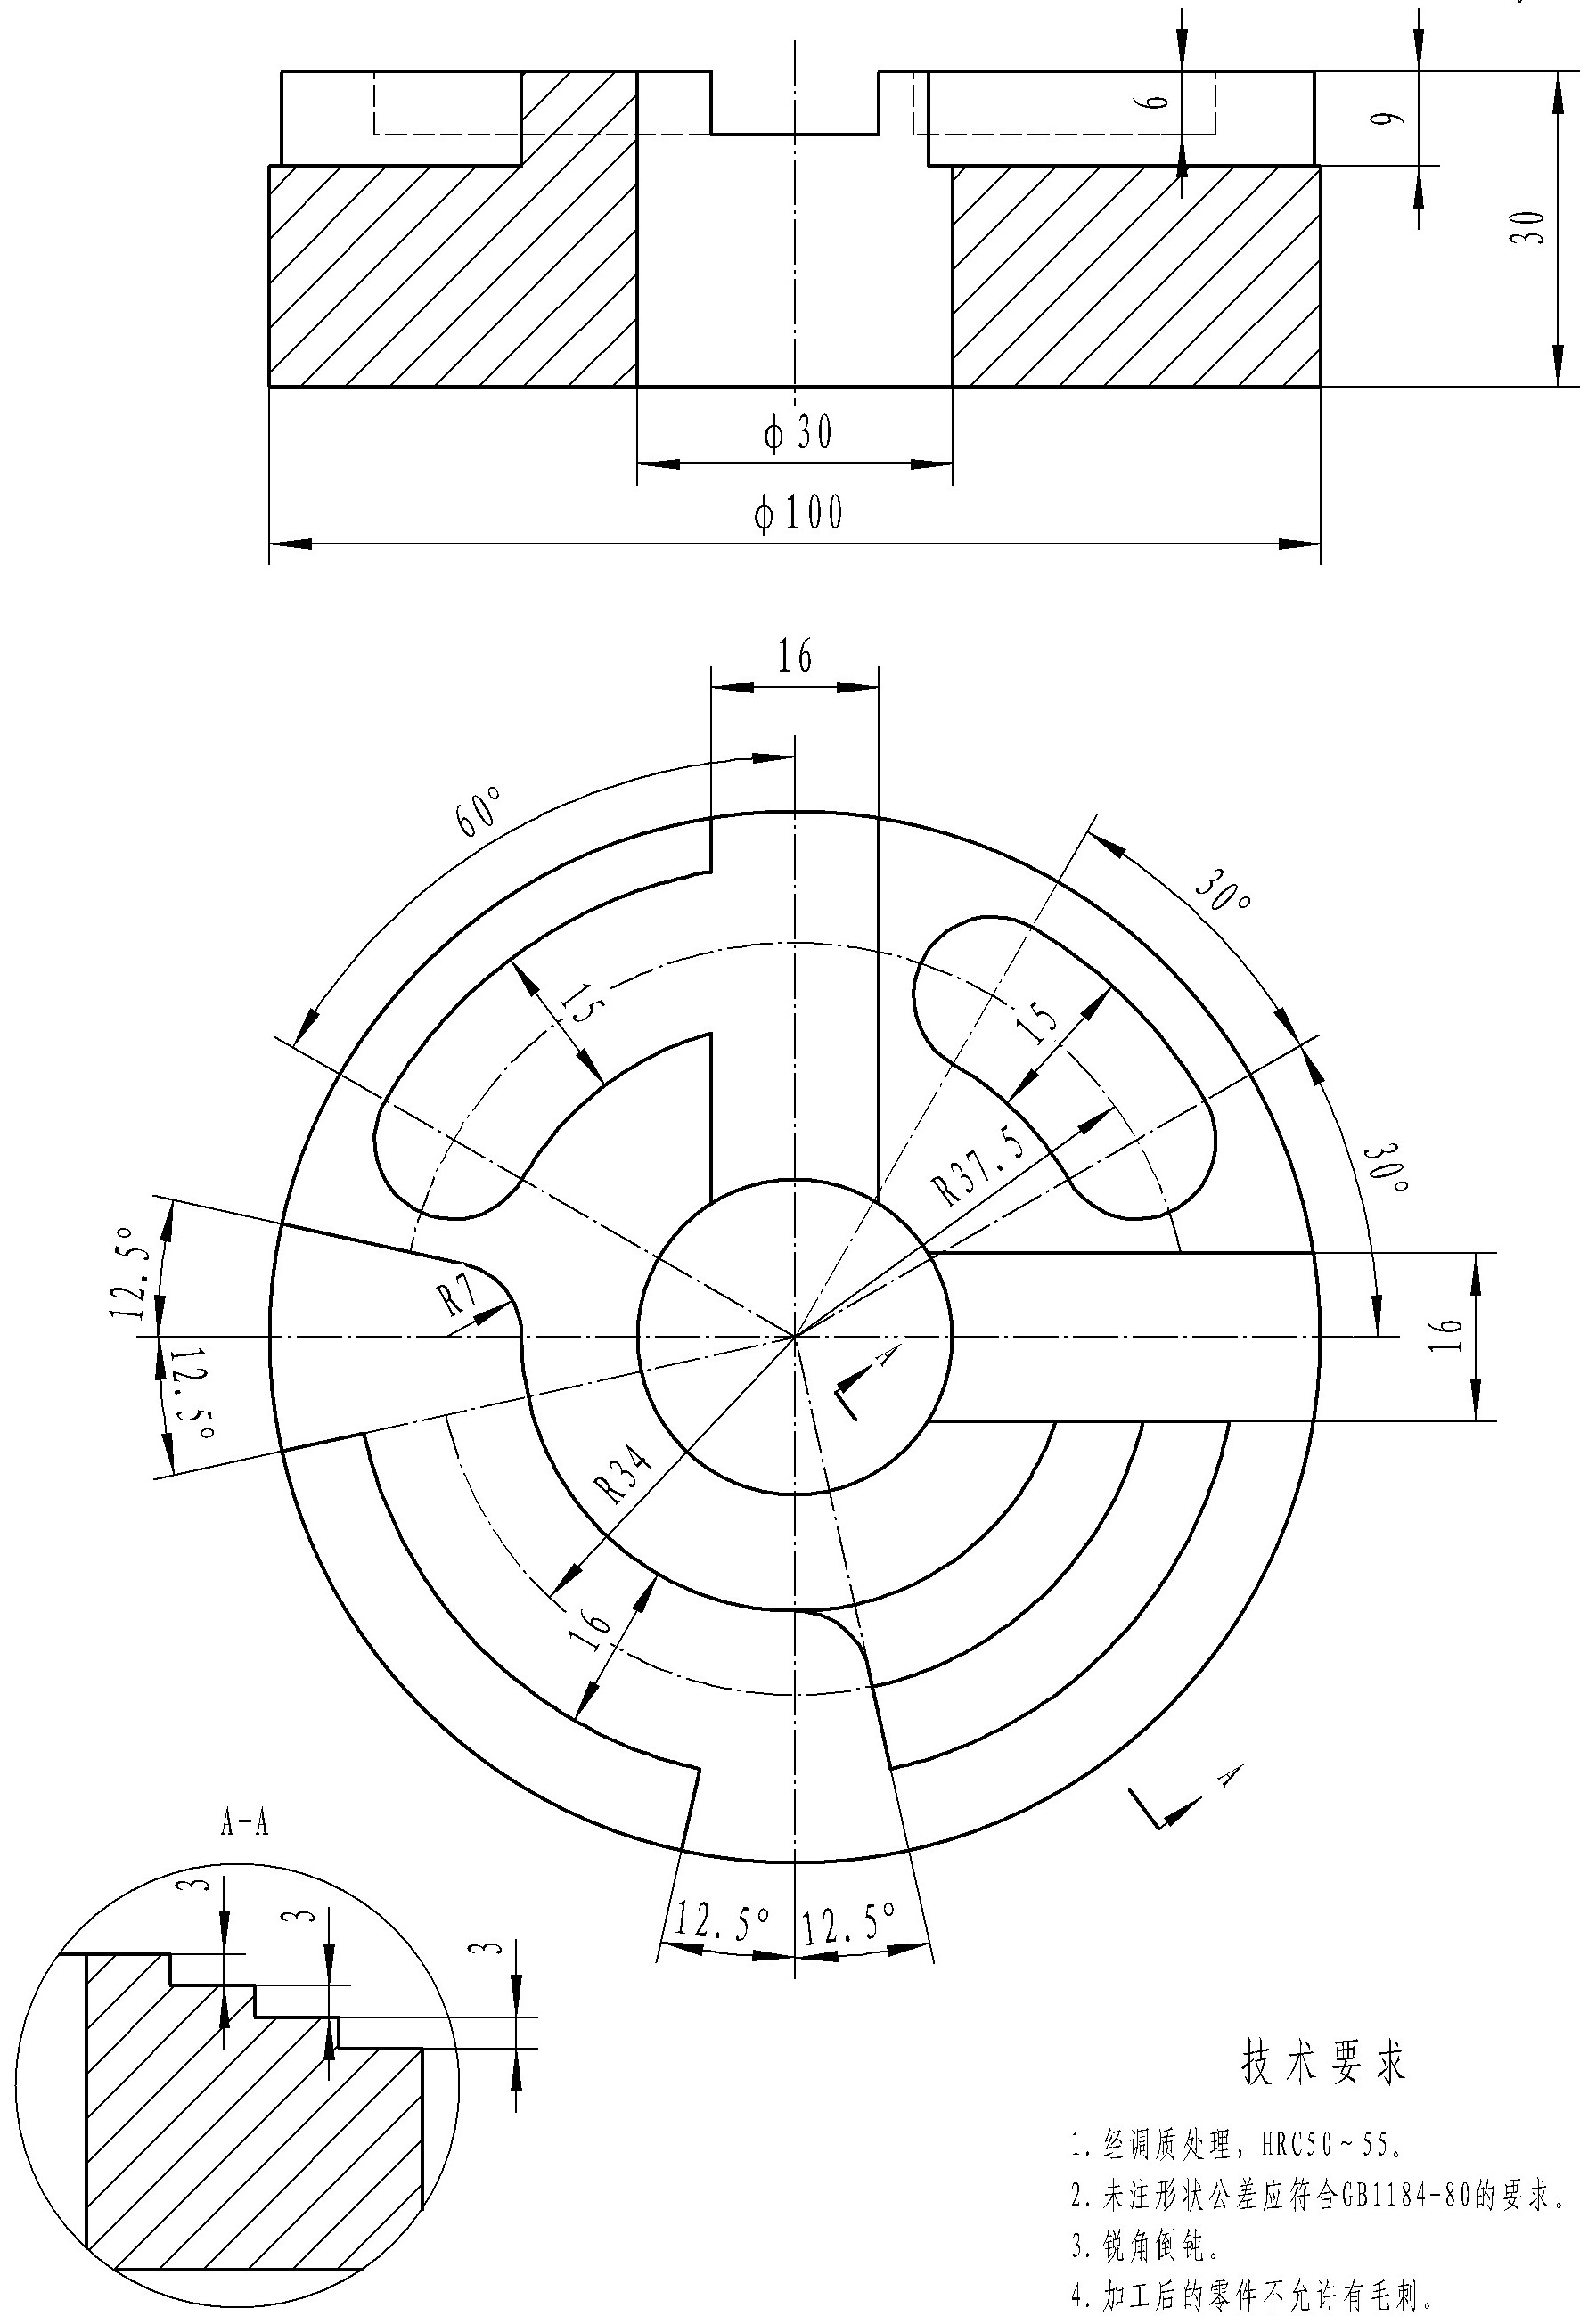
\includegraphics[width=0.8\textwidth]{images/9-1}
	\caption{极坐标实例} \label{极坐标实例}
\end{figure}
\textbf{加工轮廓的处理(改路径,延长)}
\paragraph{把加工轮廓进行拆分}
\noindent A、两个直槽:\\
标点的坐标,直角坐标(开放的)\\
B、小圆弧槽:\\
标点的坐标,使用极坐标\\
C、腰形槽:\\
标点的坐标,极坐标\\
D、扇形台阶\\
标点的坐标,极坐标\\
起点与终点不重合\\
编程时的处理\\
E、带翅膀的圆弧槽。
\paragraph{极坐标与 直角坐标的互换}
$$X=P*cosA$$
$$Y=P*sinA$$
$$P=X2+Y2$$
$$A=aictanY/X$$
\subsubsection{极坐标}
\paragraph{Fanuc上的极坐标}
指令格式: G\_\_ G~~ G16;启动极坐标指令(极坐标方式)\\
G~~ IP\_\_; 极坐标指令\\
:\\
G15;取消极坐标\\
说明:G\_\_极坐标指令的平面选择(G17、G18、G19)\\
G~~ G90指定工件坐标系的零点作为极坐标系原点,\\
G91指定当前位置作为极坐标系的原点。\\
IP\_\_指定极坐标系选择平面的轴地址及其值。\\
第1轴:极坐标半径\\
第2轴:极坐标角度 \\
用G90指定半径,极点设在工件坐标系原点。\\
如再用G90指定角度,角度是与X轴的夹角\\
如再用G91指定角度,角度是与当前位置的夹角\\
用G91指定半径,极点设在刀具当前位置。\\
如再用G90指定角度,角度是与X轴的夹角\\
如再用G91指定角度,角度是与当前位置的夹角。\\
限制:A、在极坐标方式中,对圆弧插补或螺旋线插补(G02,G03)用R 指定半径。\\
在极坐标方式中,不能用以下指令:\\
G4、G10、G52、G92、G53、G68、G51\\
在极坐标方式中不能倒角和倒圆\\
\paragraph{Siemens上的极坐标}
\textbf{极坐标,极点定义}:G110,G111,G112 \\
A、在直角坐标系中定义极点:\\
G110/G111/G112 X\_\_ Y\_\_ Z\_\_\\
B、在极坐标系中定义极点:\\
G110/G111/G112 AP=\_\_RP=\_\_\\
说明: \\
G110:相对于刀具最近到达的点(刀具当前位置)定义极点\\
G111:相对于当前工件坐标系定义极点\\
G112:相对于上一个有效极点定义极点\\
\textbf{在极坐标系中使用极坐标}\\
A、G0 AP=\_\_ RP=\_\_\\
B、G1 AP=\_\_ RP=\_\_\\
C、G2 AP=\_\_RP=\_\_\\
D、G3 AP=\_\_ RP=\_\_
说明:\\
AP=\_\_:极角,极点和目标点之间连线与角度参考方向之间的夹角(第一次角度参考方向线中一条),取值范围±(0-360),当用绝对坐标编程时,角度为相对于加工平面的水平轴方向,当用相对坐标编程时,上一个被编程角度作为参考位置。极角一直保持到新的极角被定义或工件坐标系被改变。\\
RP=\_\_:极半径,极点和目标点之间的距离,极半径一保持到新的极半径被定义。\\
所有与极坐标有关的输入必须在单个程序段内编程。用极坐标所定义的位置都可以用G0 G1 G2 G3去移动,极坐系在由G17/G18/G19所定义的加工平面内都有效。如果没有极坐标在使用,有效的工件坐标系的原点有用,\\
\subsubsection{加工工序} \marginpar{ 比较分析讲解}
A、铣上表面\\
B、铣ф30通孔(也可钻、扩、镗)\\
C、铣直槽和圆弧\\
……
由学生自己分析。\\


















\subsection{课堂小结}
\begin{enumerate}[1、]
	\item 加工轮廓的处理;
	\item 极坐标;
	\item 加工工序。
\end{enumerate}

\vfill
\subsection{布置作业}
\begin{enumerate}[1、]
	\item 自选一零件图, 写出其工艺与程序。 
\end{enumerate}
\vfill
\jxhj{%教学后记
	}
\skrq{%授课日期
	2017年5月9日 4-5节}
\ktmq{%课题名称
	 极坐标指令}
\jxmb{%教学目标,每行前面要加 \item
	\item 掌握Fanuc上极坐标指令的使用;
	\item 掌握Siemens上极坐标指令的使用;
	\item 灵活使用极坐标指令进行编程;
	\item 掌握加工工艺的分析。 }
\jxzd{%教学重点,每行前面要加 \item
	\item 极坐标知识和其指令的使用;
	\item 对加工轮廓进行处理后再编程。 }
\jxnd{%教学难点,每行前面要加 \item
	\item 加工轮廓进行处理后再编程。 }
\jjff{%教学方法
	通过讲述、举例、演示法来说明;}

\makeshouye %制作教案首页

%%%%教学内容
\subsection{组织教学}
\begin{enumerate}[\hspace{2em}1、]
	\item 集中学生注意力;
	\item 清查学生人数;
	\item 维持课堂纪律;
\end{enumerate}
\subsection{复习导入及主要内容}
\begin{enumerate}[1、]
	\item 旋转可应用场合;
	\item 要素及原理;
	\item Fanuc旋转指令格式;
	\item Sienes旋转指令格式;
	\item 编程实例。
\end{enumerate}



\subsection{教学内容及过程}

\subsubsection{加工轮廓的处理}
\begin{figure}[!hbtp]
	\centering	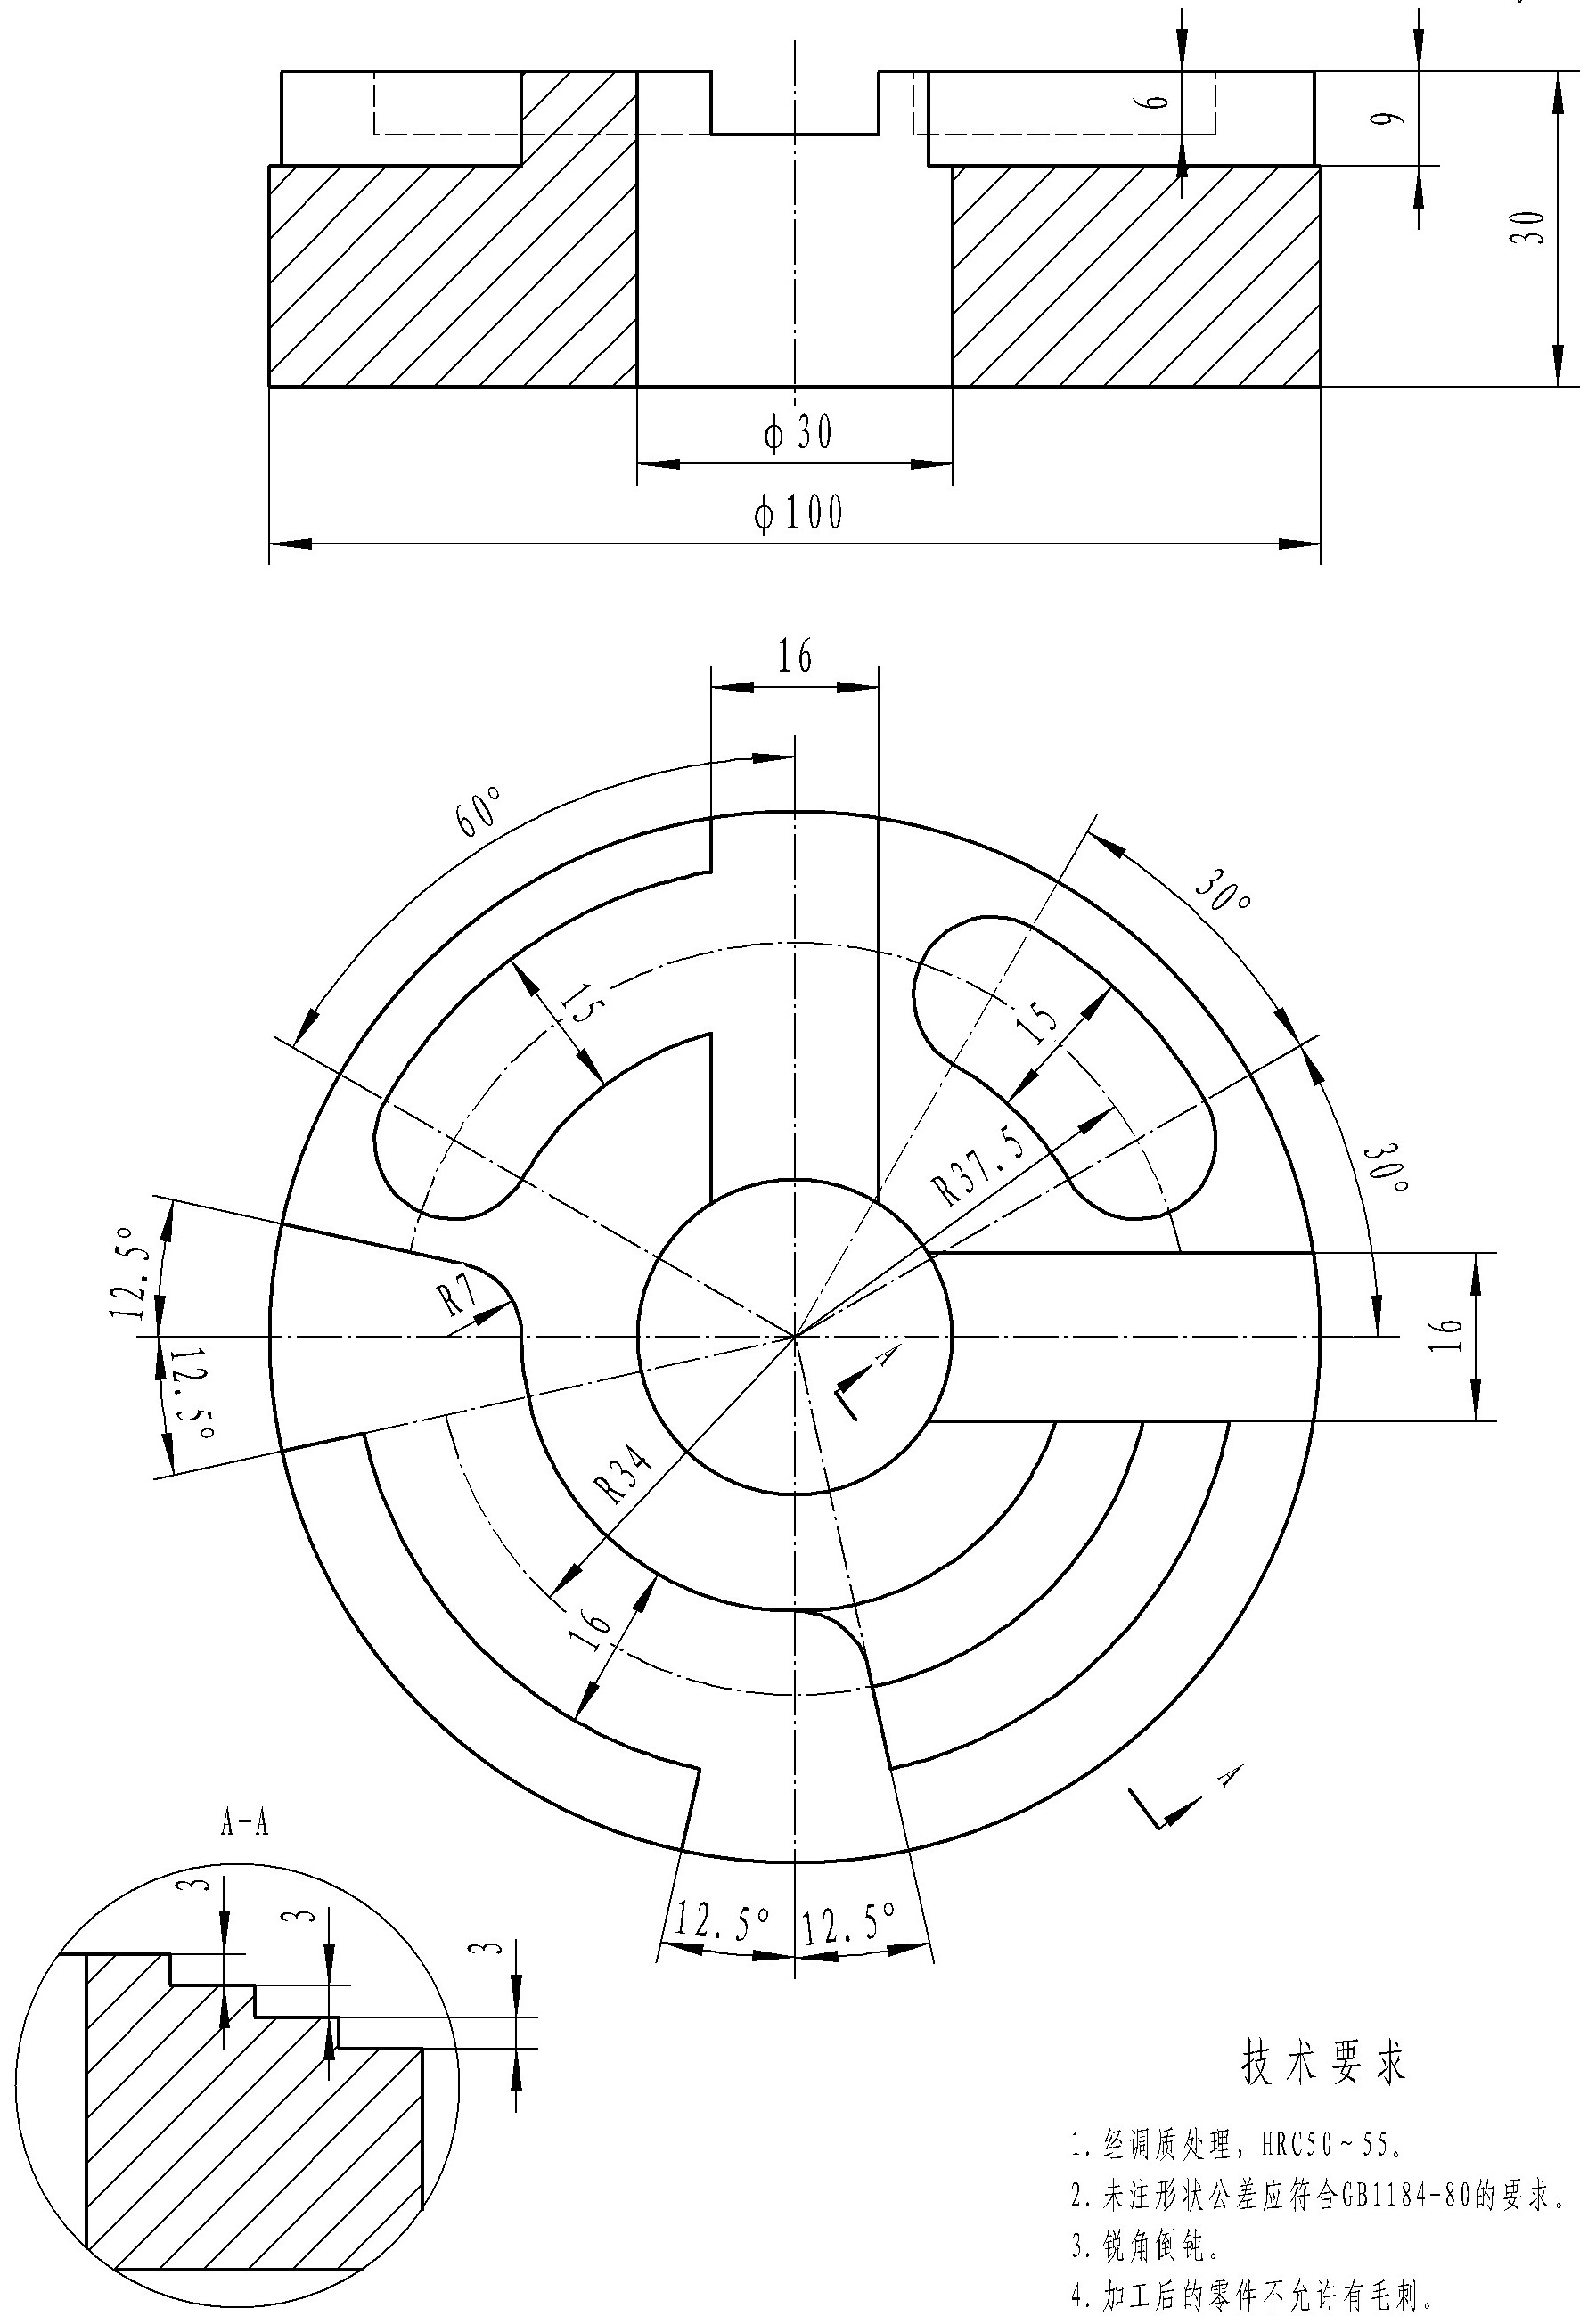
\includegraphics[width=0.8\textwidth]{images/9-1}
	\caption{极坐标实例} \label{极坐标实例}
\end{figure}
\textbf{加工轮廓的处理(改路径,延长)}
\paragraph{把加工轮廓进行拆分}
\noindent A、两个直槽:\\
标点的坐标,直角坐标(开放的)\\
B、小圆弧槽:\\
标点的坐标,使用极坐标\\
C、腰形槽:\\
标点的坐标,极坐标\\
D、扇形台阶\\
标点的坐标,极坐标\\
起点与终点不重合\\
编程时的处理\\
E、带翅膀的圆弧槽。
\paragraph{极坐标与 直角坐标的互换}
$$X=P*cosA$$
$$Y=P*sinA$$
$$P=X2+Y2$$
$$A=aictanY/X$$
\subsubsection{极坐标}
\paragraph{Fanuc上的极坐标}
指令格式: G\_\_ G~~ G16;启动极坐标指令(极坐标方式)\\
G~~ IP\_\_; 极坐标指令\\
:\\
G15;取消极坐标\\
说明:G\_\_极坐标指令的平面选择(G17、G18、G19)\\
G~~ G90指定工件坐标系的零点作为极坐标系原点,\\
G91指定当前位置作为极坐标系的原点。\\
IP\_\_指定极坐标系选择平面的轴地址及其值。\\
第1轴:极坐标半径\\
第2轴:极坐标角度 \\
用G90指定半径,极点设在工件坐标系原点。\\
如再用G90指定角度,角度是与X轴的夹角\\
如再用G91指定角度,角度是与当前位置的夹角\\
用G91指定半径,极点设在刀具当前位置。\\
如再用G90指定角度,角度是与X轴的夹角\\
如再用G91指定角度,角度是与当前位置的夹角。\\
限制:A、在极坐标方式中,对圆弧插补或螺旋线插补(G02,G03)用R 指定半径。\\
在极坐标方式中,不能用以下指令:\\
G4、G10、G52、G92、G53、G68、G51\\
在极坐标方式中不能倒角和倒圆\\
\paragraph{Siemens上的极坐标}
\textbf{极坐标,极点定义}:G110,G111,G112 \\
A、在直角坐标系中定义极点:\\
G110/G111/G112 X\_\_ Y\_\_ Z\_\_\\
B、在极坐标系中定义极点:\\
G110/G111/G112 AP=\_\_RP=\_\_\\
说明: \\
G110:相对于刀具最近到达的点(刀具当前位置)定义极点\\
G111:相对于当前工件坐标系定义极点\\
G112:相对于上一个有效极点定义极点\\
\textbf{在极坐标系中使用极坐标}\\
A、G0 AP=\_\_ RP=\_\_\\
B、G1 AP=\_\_ RP=\_\_\\
C、G2 AP=\_\_RP=\_\_\\
D、G3 AP=\_\_ RP=\_\_
说明:\\
AP=\_\_:极角,极点和目标点之间连线与角度参考方向之间的夹角(第一次角度参考方向线中一条),取值范围±(0-360),当用绝对坐标编程时,角度为相对于加工平面的水平轴方向,当用相对坐标编程时,上一个被编程角度作为参考位置。极角一直保持到新的极角被定义或工件坐标系被改变。\\
RP=\_\_:极半径,极点和目标点之间的距离,极半径一保持到新的极半径被定义。\\
所有与极坐标有关的输入必须在单个程序段内编程。用极坐标所定义的位置都可以用G0 G1 G2 G3去移动,极坐系在由G17/G18/G19所定义的加工平面内都有效。如果没有极坐标在使用,有效的工件坐标系的原点有用,\\
\subsubsection{加工工序} \marginpar{ 比较分析讲解}
A、铣上表面\\
B、铣ф30通孔(也可钻、扩、镗)\\
C、铣直槽和圆弧\\
……
由学生自己分析。\\


















\subsection{课堂小结}
\begin{enumerate}[1、]
	\item 加工轮廓的处理;
	\item 极坐标;
	\item 加工工序。
\end{enumerate}

\vfill
\subsection{布置作业}
\begin{enumerate}[1、]
	\item 自选一零件图, 写出其工艺与程序。 
\end{enumerate}
\vfill
\jxhj{%教学后记
	}
\skrq{%授课日期
	2017年5月16日 4-5节}
\ktmq{%课题名称
	 极坐标指令}
\jxmb{%教学目标,每行前面要加 \item
	\item 掌握Fanuc上极坐标指令的使用;
	\item 掌握Siemens上极坐标指令的使用;
	\item 灵活使用极坐标指令进行编程;
	\item 掌握加工工艺的分析。 }
\jxzd{%教学重点,每行前面要加 \item
	\item 极坐标知识和其指令的使用;
	\item 对加工轮廓进行处理后再编程。 }
\jxnd{%教学难点,每行前面要加 \item
	\item 加工轮廓进行处理后再编程。 }
\jjff{%教学方法
	通过讲述、举例、演示法来说明;}

\makeshouye %制作教案首页

%%%%教学内容
\subsection{组织教学}
\begin{enumerate}[\hspace{2em}1、]
	\item 集中学生注意力;
	\item 清查学生人数;
	\item 维持课堂纪律;
\end{enumerate}
\subsection{复习导入及主要内容}
\begin{enumerate}[1、]
	\item 旋转可应用场合;
	\item 要素及原理;
	\item Fanuc旋转指令格式;
	\item Sienes旋转指令格式;
	\item 编程实例。
\end{enumerate}



\subsection{教学内容及过程}

\subsubsection{加工轮廓的处理}
\begin{figure}
	\centering	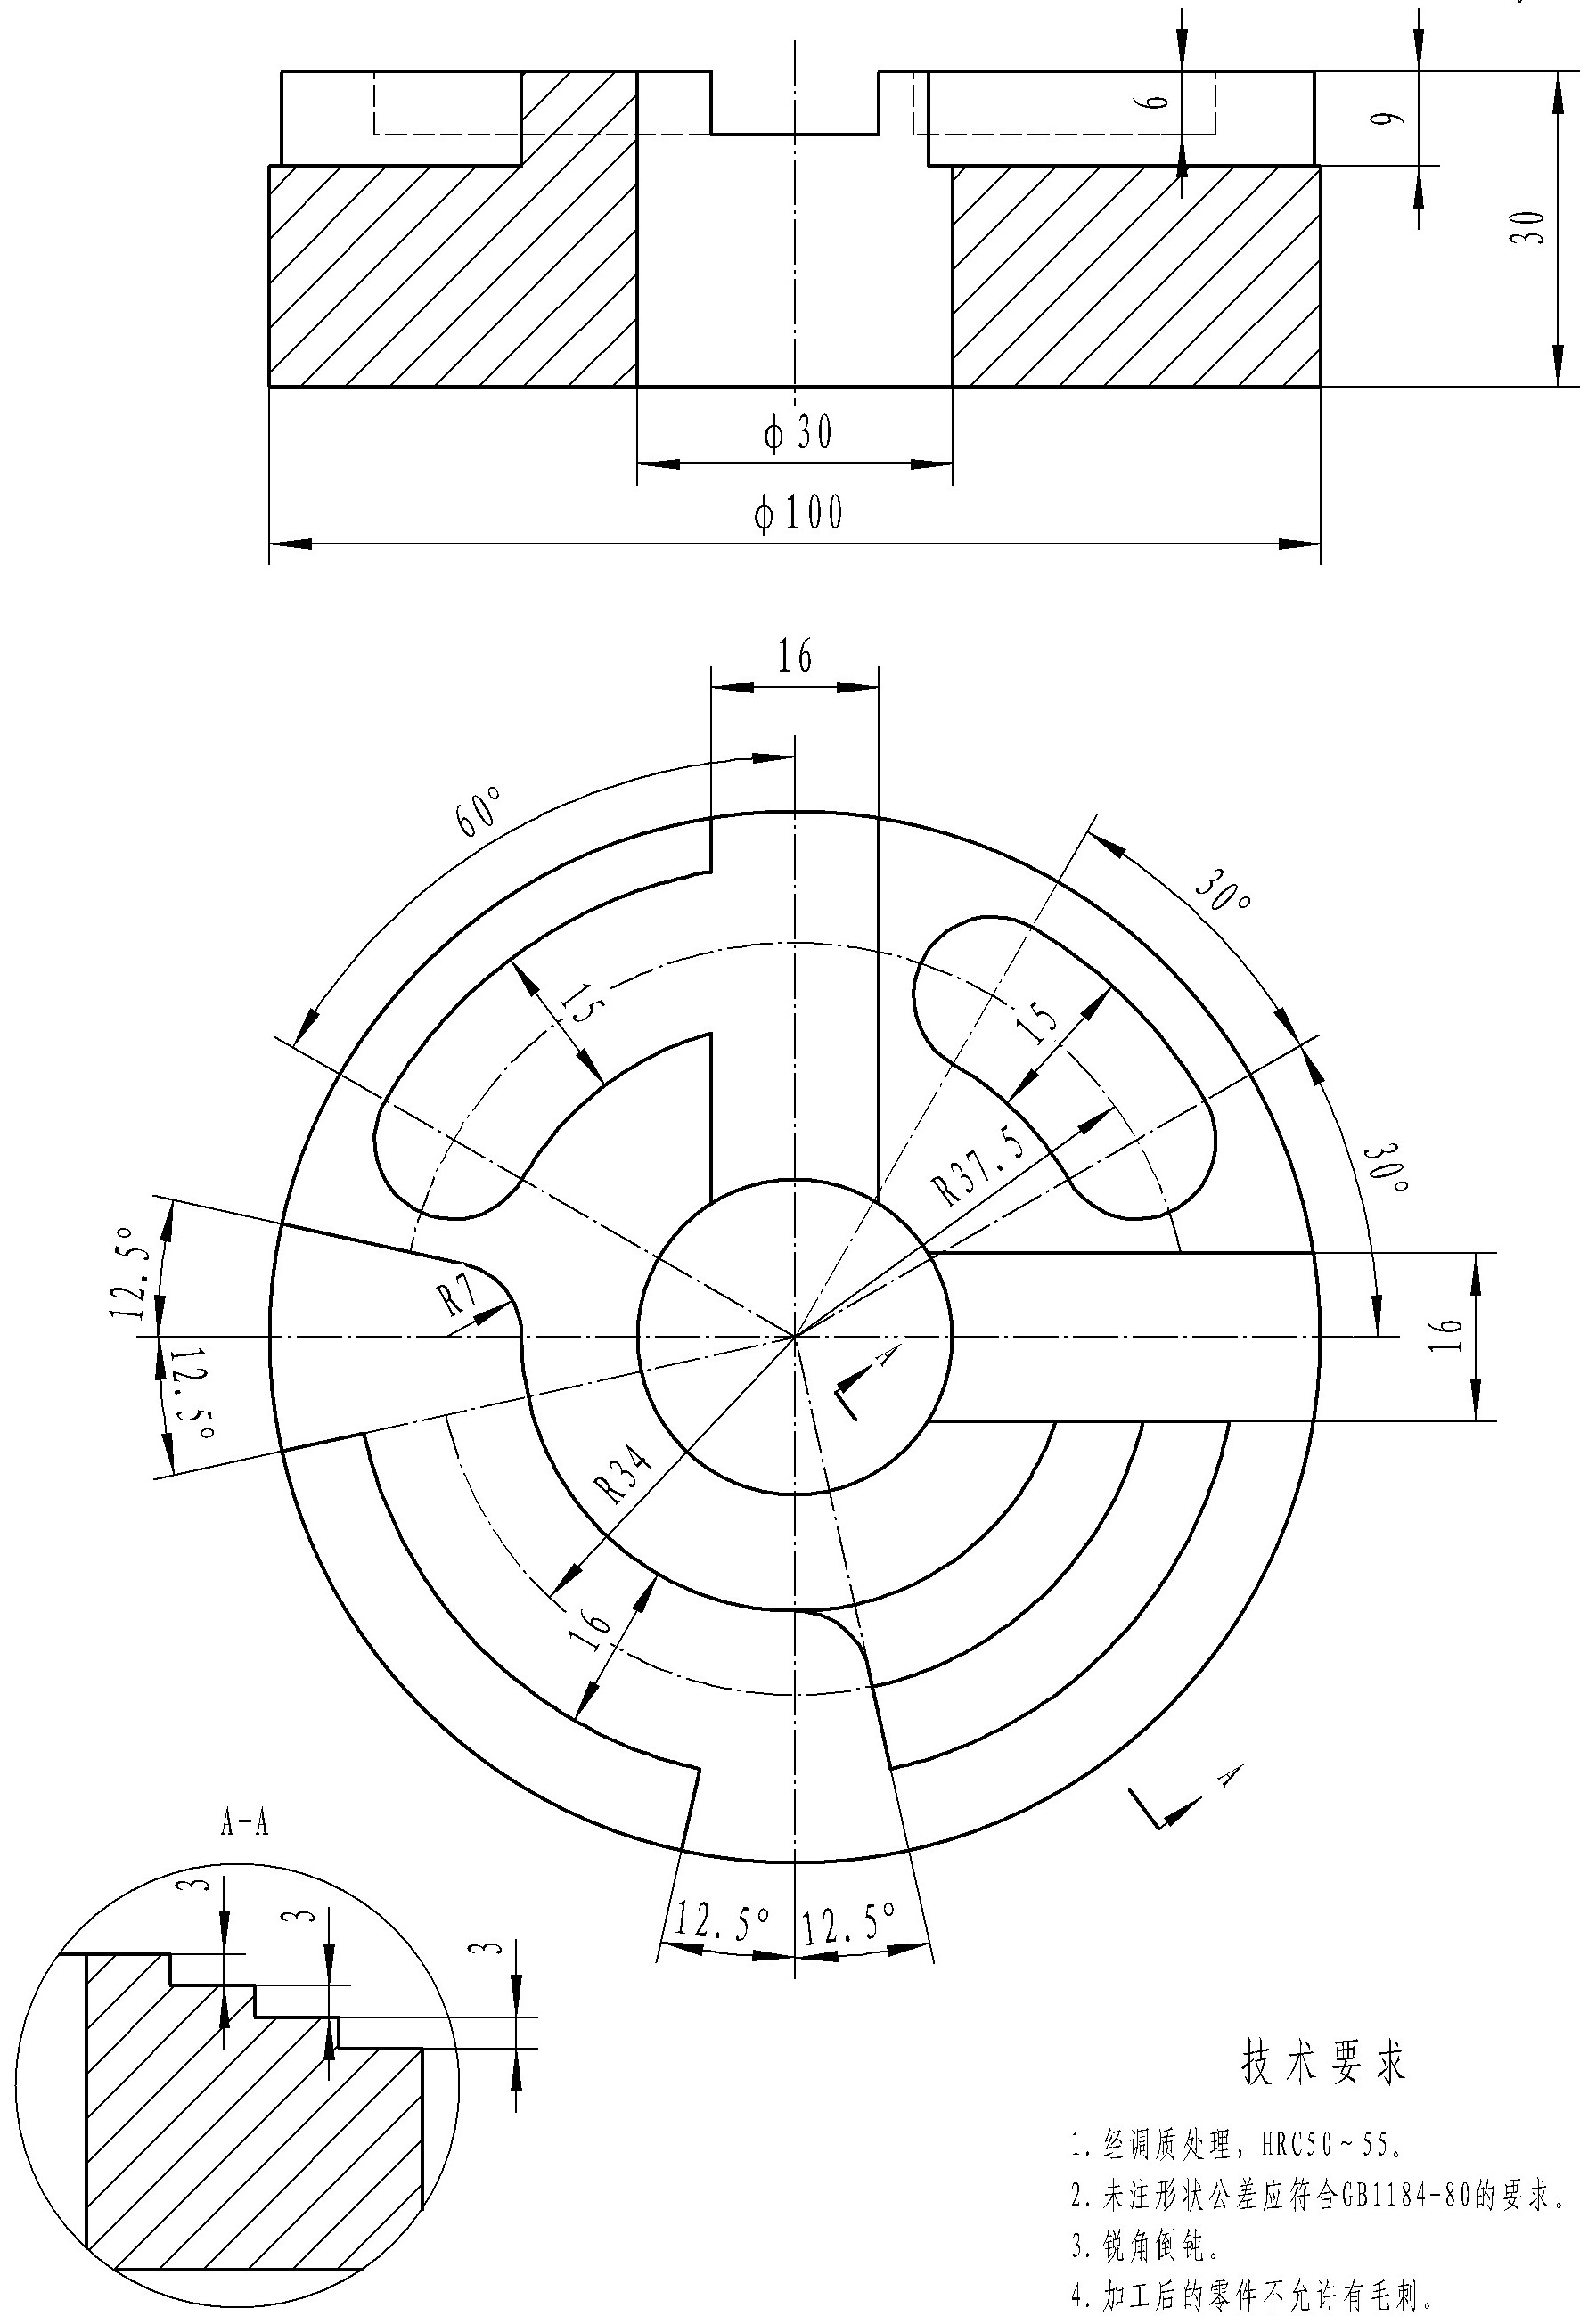
\includegraphics[width=0.8\textwidth]{images/9-1}
	\caption{极坐标实例} \label{极坐标实例}
\end{figure}
\textbf{加工轮廓的处理(改路径,延长)}
\paragraph{把加工轮廓进行拆分}
\noindent A、两个直槽:\\
标点的坐标,直角坐标(开放的)\\
B、小圆弧槽:\\
标点的坐标,使用极坐标\\
C、腰形槽:\\
标点的坐标,极坐标\\
D、扇形台阶\\
标点的坐标,极坐标\\
起点与终点不重合\\
编程时的处理\\
E、带翅膀的圆弧槽。
\paragraph{极坐标与 直角坐标的互换}
$$X=P*cosA$$
$$Y=P*sinA$$
$$P=X2+Y2$$
$$A=aictanY/X$$
\subsubsection{极坐标}
\paragraph{Fanuc上的极坐标}
指令格式: G\_\_ G~~ G16;启动极坐标指令(极坐标方式)\\
G~~ IP\_\_; 极坐标指令\\
:\\
G15;取消极坐标\\
说明:G\_\_极坐标指令的平面选择(G17、G18、G19)\\
G~~ G90指定工件坐标系的零点作为极坐标系原点,\\
G91指定当前位置作为极坐标系的原点。\\
IP\_\_指定极坐标系选择平面的轴地址及其值。\\
第1轴:极坐标半径\\
第2轴:极坐标角度 \\
用G90指定半径,极点设在工件坐标系原点。\\
如再用G90指定角度,角度是与X轴的夹角\\
如再用G91指定角度,角度是与当前位置的夹角\\
用G91指定半径,极点设在刀具当前位置。\\
如再用G90指定角度,角度是与X轴的夹角\\
如再用G91指定角度,角度是与当前位置的夹角。\\
限制:A、在极坐标方式中,对圆弧插补或螺旋线插补(G02,G03)用R 指定半径。\\
在极坐标方式中,不能用以下指令:\\
G4、G10、G52、G92、G53、G68、G51\\
在极坐标方式中不能倒角和倒圆\\
\paragraph{Siemens上的极坐标}
\textbf{极坐标,极点定义}:G110,G111,G112 \\
A、在直角坐标系中定义极点:\\
G110/G111/G112 X\_\_ Y\_\_ Z\_\_\\
B、在极坐标系中定义极点:\\
G110/G111/G112 AP=\_\_RP=\_\_\\
说明: \\
G110:相对于刀具最近到达的点(刀具当前位置)定义极点\\
G111:相对于当前工件坐标系定义极点\\
G112:相对于上一个有效极点定义极点\\
\textbf{在极坐标系中使用极坐标}\\
A、G0 AP=\_\_ RP=\_\_\\
B、G1 AP=\_\_ RP=\_\_\\
C、G2 AP=\_\_RP=\_\_\\
D、G3 AP=\_\_ RP=\_\_
说明:\\
AP=\_\_:极角,极点和目标点之间连线与角度参考方向之间的夹角(第一次角度参考方向线中一条),取值范围±(0-360),当用绝对坐标编程时,角度为相对于加工平面的水平轴方向,当用相对坐标编程时,上一个被编程角度作为参考位置。极角一直保持到新的极角被定义或工件坐标系被改变。\\
RP=\_\_:极半径,极点和目标点之间的距离,极半径一保持到新的极半径被定义。\\
所有与极坐标有关的输入必须在单个程序段内编程。用极坐标所定义的位置都可以用G0 G1 G2 G3去移动,极坐系在由G17/G18/G19所定义的加工平面内都有效。如果没有极坐标在使用,有效的工件坐标系的原点有用,\\
\subsubsection{加工工序} \marginpar{ 比较分析讲解}
A、铣上表面\\
B、铣ф30通孔(也可钻、扩、镗)\\
C、铣直槽和圆弧\\
……
由学生自己分析。\\


















\subsection{课堂小结}
\begin{enumerate}[1、]
	\item 加工轮廓的处理;
	\item 极坐标;
	\item 加工工序。
\end{enumerate}

\vfill
\subsection{布置作业}
\begin{enumerate}[1、]
	\item 自选一零件图, 写出其工艺与程序。 
\end{enumerate}
\vfill
\jxhj{%教学后记
	}
\skrq{%授课日期
	2017年5月22日 4-5节}
\ktmq{%课题名称
	 变量周边倒圆角}
\jxmb{%教学目标,每行前面要加 \item
	\item 掌握简单零件的倒圆;
	\item 掌握相关数学处理;
	\item 掌握循环的几个特点;
	\item 掌握简单零件的倒角。 }
\jxzd{%教学重点,每行前面要加 \item
	\item 掌握简单零件的倒圆;
	\item 掌握简单零件的倒角。 }
\jxnd{%教学难点,每行前面要加 \item
	\item 相关数学处理。 }
\jjff{%教学方法
	通过讲述、举例、演示法来说明;}

\makeshouye %制作教案首页

%%%%教学内容
\subsection{组织教学}
\begin{enumerate}[\hspace{2em}1、]
	\item 集中学生注意力;
	\item 清查学生人数;
	\item 维持课堂纪律;
\end{enumerate}
\subsection{复习导入及主要内容}
\begin{enumerate}[1、]
	\item 加工轮廓的处理;
	\item 极坐标;
	\item 加工工序。
\end{enumerate}


\subsection{教学内容及过程}

\subsubsection{简单零件的倒角}
如图\ref{园锥}所示:
\begin{figure}[!hbtp]
	\centering	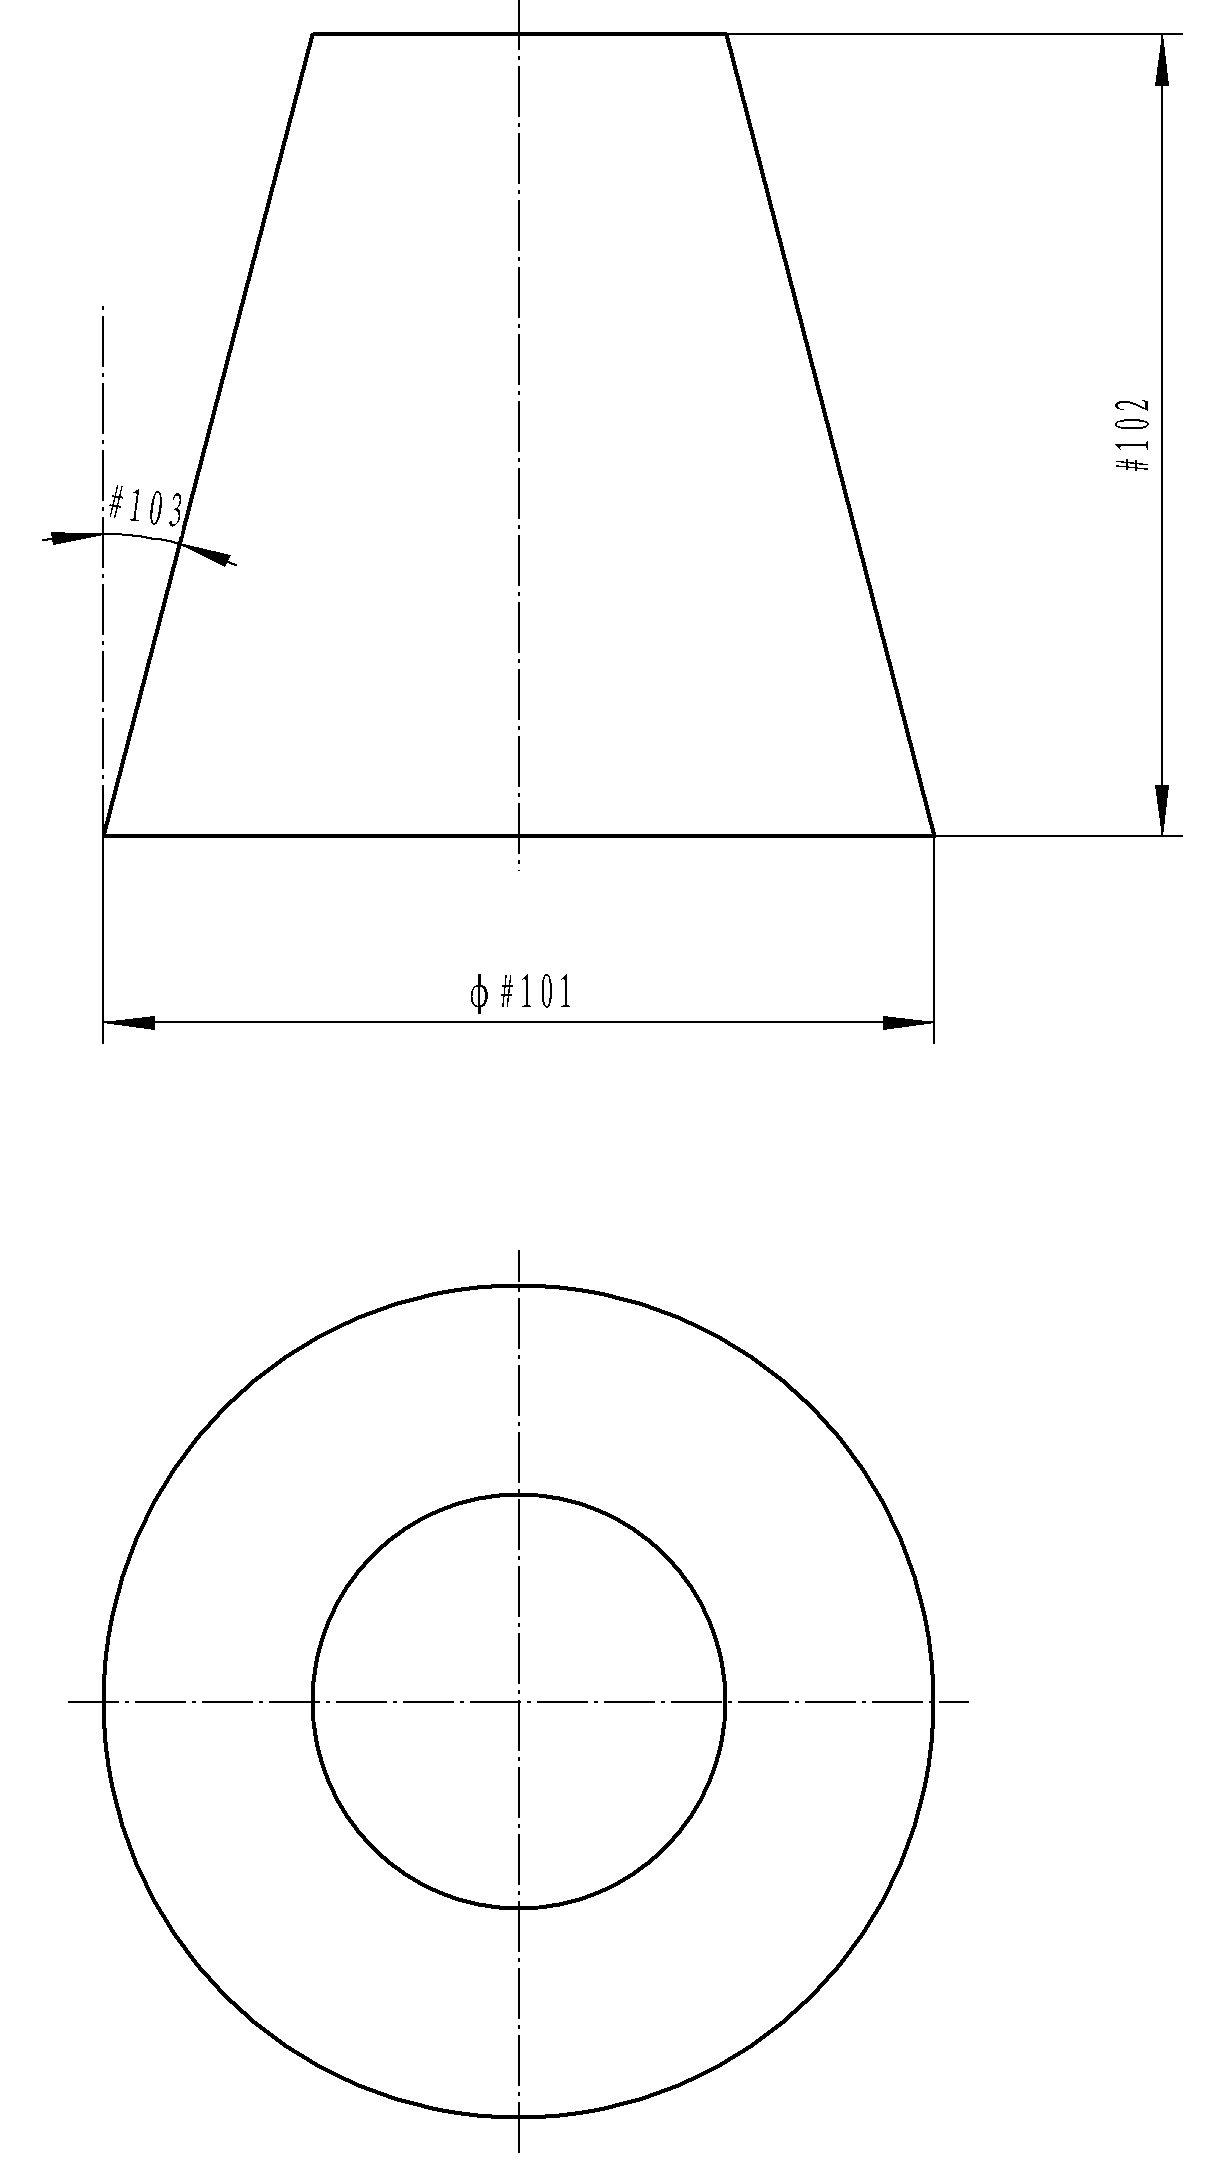
\includegraphics[width=0.4\textwidth]{images/13-1.jpg}
	\caption{圆锥} \label{圆锥}
\end{figure}
参考程序:
\begin{lstlisting}
O0001
#101=50
#102=20
#103=15
#104=8
#105=0.1
G54G17G40G49G90
M3S500
G1Z30.F2000
X-[#101/2+#104]Y0
Z5.0
Z-#102F200
#120=#102
WHILE[#120 GT 0]DO1
#120=#120-#105
G1Z-#120
#121=#101/2-[#102-#120]*TAN[#103]
X-[#121+#104] Y0
G2 I[#121+#104]
END1
G1 Z30.F2000
M5
M30
\end{lstlisting}
\subsubsection{写出如图\ref{圆角}所示零件的宏程序}
\begin{figure}[!hbtp]
	\centering	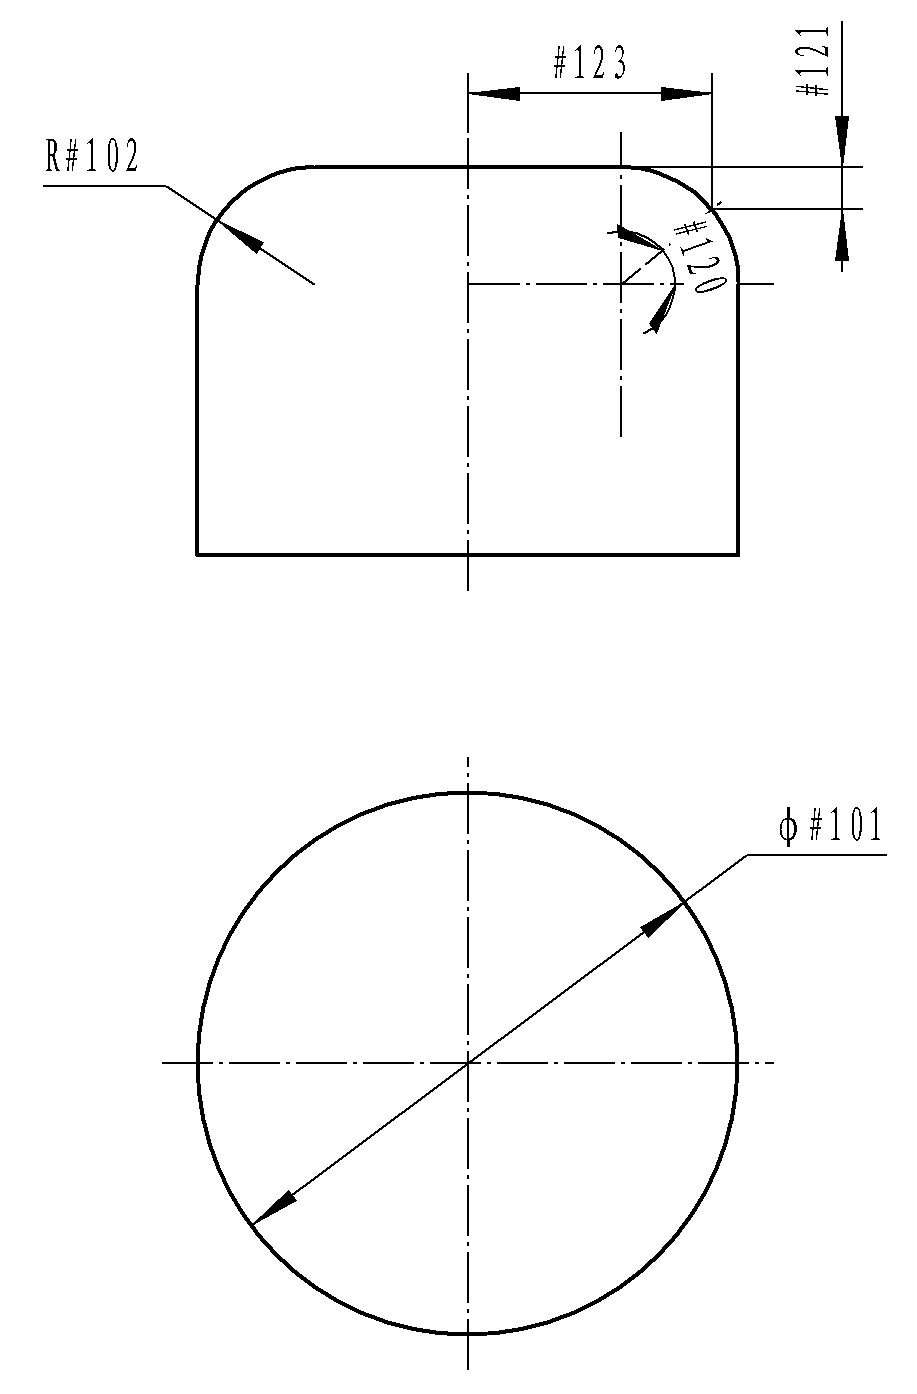
\includegraphics[width=0.4\textwidth]{images/13-2.jpg}
	\caption{圆角} \label{圆角}
\end{figure}
刀具半径: \#103

加工精度: \#104

Z向分层(用角度控制)

初始值: \#120=0

终止值: 90

\verb|#121=#102-#102*sin[#120]|

\verb|#122=#101/2-[#102-#102*cos[#120]]|

参考程序:
\begin{lstlisting}
O0001
#101----#104
G54G17G40G49G90
M3S500
G1Z30.F2000
X-[#101/2+#103+1]Y0
Z5.0
Z-#102F200
#120=0
WHILE[#120LT90]DO1
#120=#120+#104
#121=#102-#102*sin[#120]
G1Z-#121
#122=#101/2-[#102-#102*cos[#120]]
G1X-[#122+#103]Y0
G2I[#122+#103]
END1
G1Z30.F2000
M5
M30
\end{lstlisting}
\subsubsection{写出如图\ref{圆角:圆锥}所示零件的宏程序}:
\begin{figure}[!hbtp]
	\centering	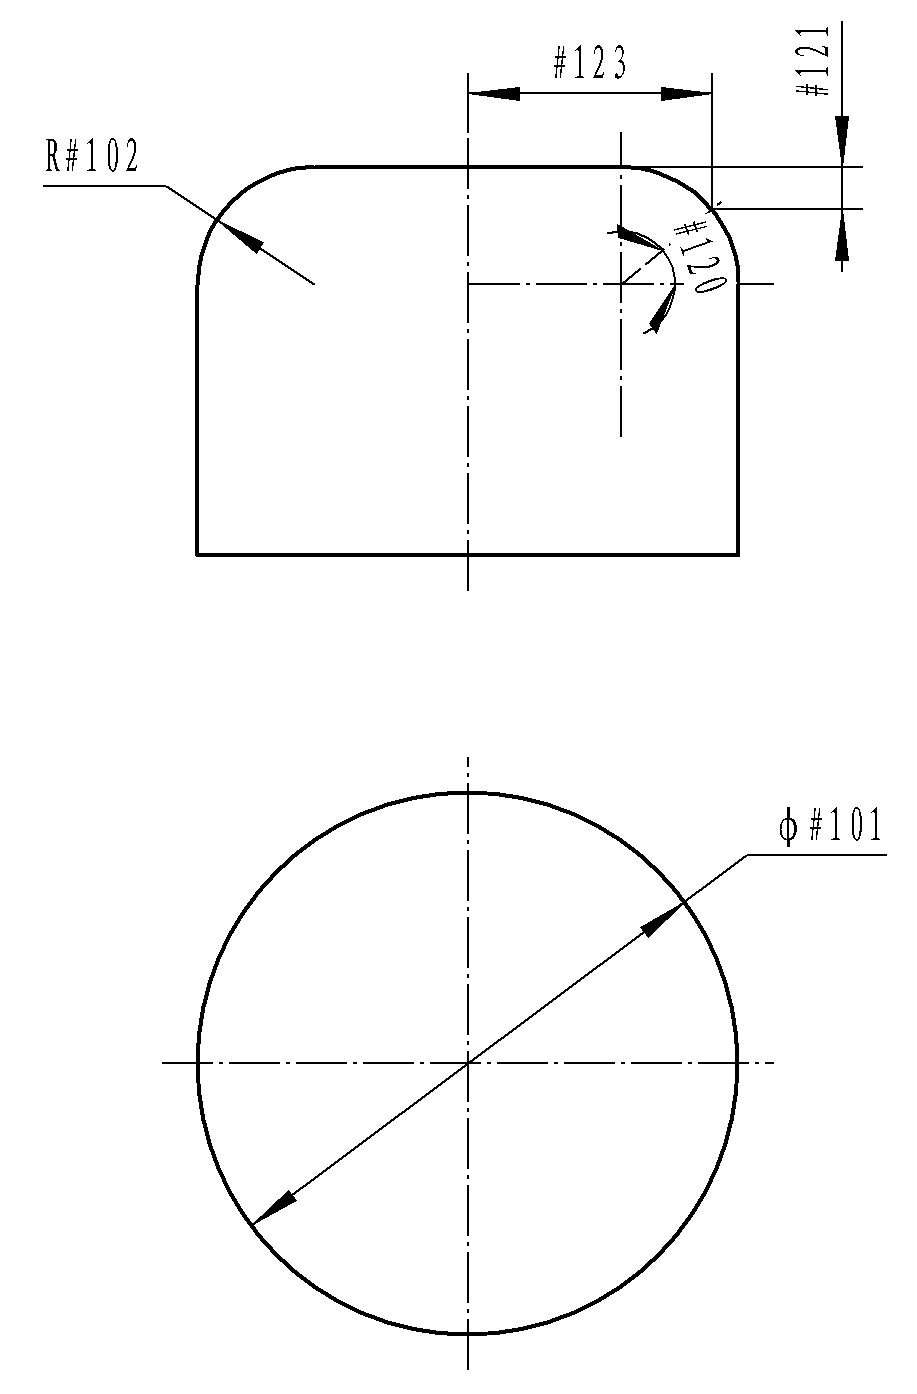
\includegraphics[width=0.4\textwidth]{images/13-2.jpg}
	\caption{圆角:圆锥} \label{圆角:圆锥}
\end{figure}
刀具:\#105

加工精度: \#106

角度精度: \#107

斜度:

Z向分层: 用长度控制

初始值: \#121=\#102

终止值为: \#102-\#131

\#131=\#102-\#103+\#103*SIN[\#104]

\#122=\#101-[\#102-\#121]*TAN[\#121]

圆角:

Z向分层:用角度控制

初始值: \#120=\#104

终止值: 90

\#121=\#103-\#103*sin[\#120]

\#122=\#132+\#103*cos[\#120]

\#132=\#103-\#131*tan[\#103]-\#102*cos[\#103]

参考程序:

\begin{lstlisting}
O0001
#101----#107
G54G17G40G49G90
M3S500
G1Z30.F2000
X-[#101+#105+2] Y0
Z5.0
Z-#102F200
#121=#102
#131=#102-#103+#103*SIN[#104]
WHILE[#121GT#131]DO1
#121=#121-#106
IF[#121LT#131]THEN#121=#131
G1Z-#121
#122=#101-[#102-#121]*TAN[#121]
X-[#122+#105]Y0
G2I[#122+#105]
END1
#132=#103-#131*tan[#103]-#102*cos[#103]
#120=#104
WHILE[#120LT90]DO1
#120=#120+#107
IF[#120GT90]THEN#120=90
#121=#103-#103*SIN[#120]
#122=#132+#103*COS[#120]
G1Z-#121
X-[#122+#105]Y0
G2I[#122+#105]
END1
G1Z30.F2000
M5
M30
\end{lstlisting}

\subsection{课堂小结}
\begin{enumerate}[1、]
	\item 简单零件的倒角;
	\item 宏程序实例1;
	\item 宏程序实例2。
\end{enumerate}

\vfill
\subsection{布置作业}
\begin{enumerate}[1、]
	\item 写出上面的程序;
	\item 从习题集上选做一个。
\end{enumerate}
\vfill
\jxhj{%教学后记
	}
\skrq{%授课日期
	2017年5月30日 4-5节}
\ktmq{%课题名称
	 自动编程}
\jxmb{%教学目标,每行前面要加 \item
	\item 程序的传输;
	\item 程序的dnc加工;
	\item 自动编程刀路。}
\jxzd{%教学重点,每行前面要加 \item
	\item 程序的传输;
	\item 自动编程刀路。}
\jxnd{%教学难点,每行前面要加 \item
	\item 自动编程刀路。}
\jjff{%教学方法
	通过讲述、举例、演示法来说明;}

\makeshouye %制作教案首页

%%%%教学内容
\subsection{组织教学}
\begin{enumerate}[\hspace{2em}1、]
	\item 集中学生注意力;
	\item 清查学生人数;
	\item 维持课堂纪律;
\end{enumerate}
\subsection{复习导入及主要内容}
\begin{enumerate}[1、]
	\item 简单零件的倒角;
	\item 宏程序实例1;
	\item 宏程序实例2。
\end{enumerate}


\subsection{教学内容及过程}


\subsubsection{数据线的接法}
RS232通讯电缆

RS-232是美国电子工业联盟(EIA)制定的串行数据通信的接口标准,全称是EIA-RS-232(简称232,RS232)。它被广泛用于计算机串行接口外设连接。

RS-232C标准(协议),232是标识号,C代表RS232的最新一次修改(1969年),在这之前,还有RS232B、RS232A

FANUC机床25PIN    电脑 9PIN

Tx(02) ---------->---------- Rx(02)

Rx(03) ----------<---------- Tx(03)

GND(07) ------------------- GND(05)

RTS(04)-CD(08)------>------- CD(01)-CTS(08)

CTS(05) ----------<--------- DTR(04)

DSR(06)<-DTR(20)------>------ DSR(06)

屏蔽 ---------------------- 屏蔽

简化:(不能硬握手)

Tx(02) ----------->--------- Rx(02)

Rx(03) -----------<--------- Tx(03)

GND(07) ------------------- GND(05)

CD(08)-DSR(6)<-DTR(20)         CD(1)DTR(4)->DSR(6)

RTS(4)->CTS(5)                 RTS(7)->CTS(8)

屏蔽 ---------------------- 屏蔽

Siemens 9PIN      电脑9PIN  (只能使用硬握手)

Rx(02)--------<---------Tx(03)

Tx(03)-------->---------Rx(02)

DTR(04)------->---------DSR(06)

GND(05)-----------------GND(05)

DSR(06)-------<---------DTR(04)

RTS(07)-------->--------CTS(08)

CTS(08)--------<---------RTS(07)

Siemens 25PIN      电脑9PIN  (只能使用硬握手)

Rx(02)--------<---------Tx(03)

Tx(03)-------->---------Rx(02)

DTR(06)------->---------DSR(06)

GND(07)-----------------GND(05)

DSR(20)-------<---------DTR(04)

RTS(05)-------->--------CTS(08)

CTS(04)--------<---------RTS(07)

其中:

Tx 发送数据(发)          Rx接受数据(收)

DTR数据终端准备(发)     DSR数据准备好(收)

RTS请求发送          CTS清除发送

CD 数据载波检测

Tx、DTR和RTS信号是由数据终止设备(DTE)产生的,Rx、DSR、CTS、DCD信号是由数据通讯设备(DCE)产生的。

DCE(如打印机)-------DTE(如服务器)

连接两个DTE设备需要一个虚拟调制解调器来充当DCE,需交换相应的信号(TD-RD, DTR-DSR, and RTS-CTS),就是上面的接法。

握手是在通信电路建立之后,信息传输开始之前。 握手用于达成参数,如信息传输率,字母表,奇偶校验, 中断过程,和其他协议特性。

软件握手(XON/XOFF)------握手通过交换的打印机与通过在传输服务器之间的控制代码来实现的并分别接收行。 数据通讯设备的数据缓冲区满时它会发送通知服务器的打印处理器的 XOFF 暂停输出。 当缓冲区可用空间的更多的数据时发送一个 XON 字符,并且服务器将继续发送到下一个 XOFF。XON/XOFF可以工作于3线的接口

硬件握手(RTS/CTS) -----使用信号电压级别的信号进行控制,要求数据终端就绪 (DTR) 针 20 在打印机清除发送 (CTS) 针 5 和在服务器上的数据集就绪 (DSR) 6 针连接上。 当打印机数据缓冲区填充时,固定 20,DTR,电压级别从更改高为低。 这将指示服务器以停止发送数据。 当缓冲区可用空间的更多的数据时 DTR 电压级别切换高,并在服务器继续发送到下一个 DTR 电压拉。

相关参数:

•	波特率(又称鲍率): 是指从一设备发到另一设备的波特率,即每秒钟多少位元bits per second (bit/s)。典型的波特率是300, 1200, 2400, 9600, 115200, 19200等bit/s。一般通信两端设备都要设为相同的波特率,但有些设备也可以设置为自动检测波特率。

•	奇偶校验(Parity:是用来验证数据的正确性。奇偶校验一般不用,如果使用,那么既可以做奇校验(Odd Parity)也可以做偶校验(Even Parity)。奇偶校验是通过修改每一发送字节(也可以限制发送的字节)来工作的。如果不作奇偶校验,那么数据是不会被改变的。在偶校验中,因为奇偶校验位会被相应的置1或0(一般是最高位或最低位),所以数据会被改变以使得所有传送的数位(含字符的各数位和校验位)中“1”的个数为偶数;在奇校验中, 所有传送的数位(含字符的各数位和校验位)中“1”的个数为奇数。奇偶校验可以用于接受方检查传输是否发送生错误——如果某一字节中“1”的个数发生了错误,那么这个字节在传输中一定有错误发生。如果奇偶校验是正确的,那么要么没有发生错误要么发生了偶数个的错误。如果使用者选择资料长度为8位元,则因为没有多余的位元可被用来作为同位元,因此就叫做“无位元(Non Parity)”。

•	停止位:是在每个字节传输之后发送的,它用来帮助接受信号方硬件重同步,即把同步讯号与资料混和之后,使用同一条传输线来传输。比如资料11001010被传输时,资料的前后就需加入Start(Low)以及Stop(High)等两个位元,Start讯号固定为一个位元,但Stop停止位元则可以是1、1.5或者是2位元。

\subsubsection{传输过程}
设定好两边的参数:

Siemens 参数      Fanuc 参数

PC 参数

传输程序:

Fanuc:

Siemens

\%\_N\_name\_MPF    或\%\_N\_name\_SPF

;PATH=/\_DIR\_MPF

\subsubsection{DNC 在线加工}

Fanuc存储卡的使用

(一).CF卡初期格式化步骤:

1将NC的I/O频道设定为4,设定页面按【setting】进入,如图\ref{频道设定}所示:

\begin{figure}[!hbtp]
	\centering	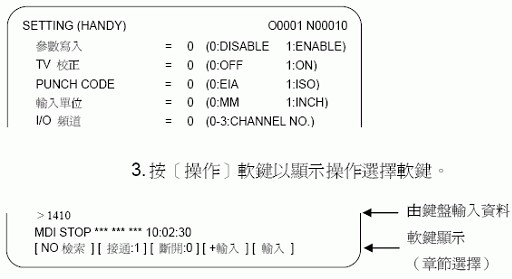
\includegraphics[width=0.9\textwidth]{images/14-1}
	\caption{频道设定} \label{频道设定}
\end{figure}

2关闭CNC系统及机台总电源;

3打开机台电控箱,将安装好的PCMCIA接口的CF卡插入到FANUC 0i主机的【CNMC】插槽,安装时注意方向,不可用力过猛;
如图\ref{插入PCMCIA卡}所示。

\begin{figure}[!hbtp]
	\centering	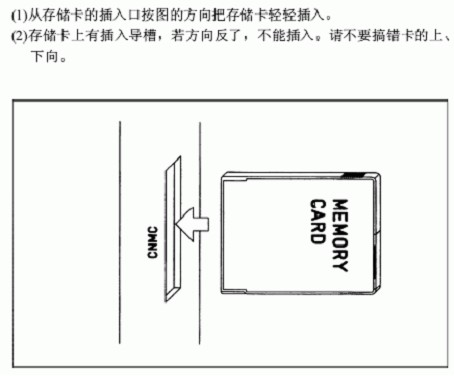
\includegraphics[width=0.9\textwidth]{images/14-2}
	\caption{插入PCMCIA卡} \label{插入PCMCIA卡}
\end{figure}

4进入NC的BOOT界面,方法为:同时按住屏幕下方最右边的两个软建,如图\ref{进入BOOT界面}所示:

\begin{figure}[!hbtp]
\centering	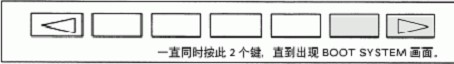
\includegraphics[width=0.9\textwidth]{images/14-3}
\caption{进入BOOT界面1} \label{进入BOOT界面}
\end{figure}

同时开启NC电源,直到出现如图\ref{进入BOOT界面1}的画面:

\begin{figure}[!hbtp]
\centering	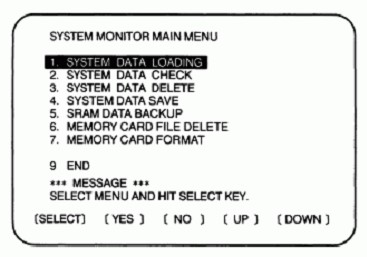
\includegraphics[width=0.9\textwidth]{images/14-4}
\centering	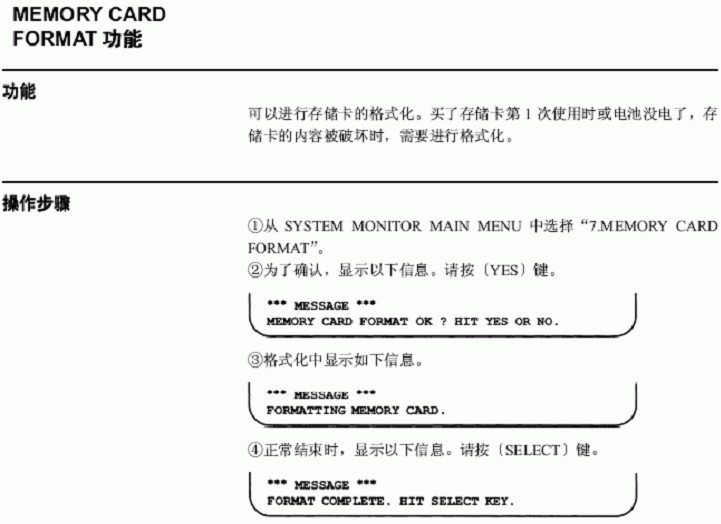
\includegraphics[width=0.9\textwidth]{images/14-5}
\caption{进入BOOT界面2} \label{进入BOOT界面1}
\end{figure}

格式化完成后,退出BOOT界面,重启系统,退出步骤如图\ref{格式化}所示:
\begin{figure}[!hbtp]
	\centering	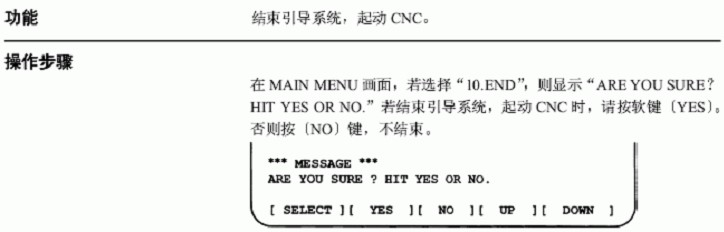
\includegraphics[width=0.9\textwidth]{images/14-6}
	\caption{格式化} \label{格式化}
\end{figure}

如果一切正常,格式过的CF卡,就可以在FANUC0i系统中使用了。如程式的存储,备份,调用等。

(二).PCMCIA卡在FANUC0i系统上的使用

Oi-MB PCMCIA读取程序操作步骤,如图\ref{读取程序操作步骤}所示。
\begin{figure}[!hbtp]
	\centering	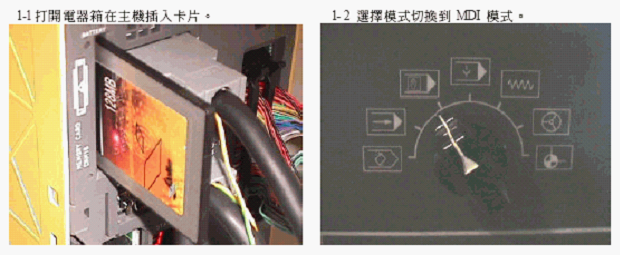
\includegraphics[width=0.8\textwidth]{images/14-7}
%	\caption{格式化} \label{格式化}
\end{figure}

\begin{figure}[!hbtp]
	\centering	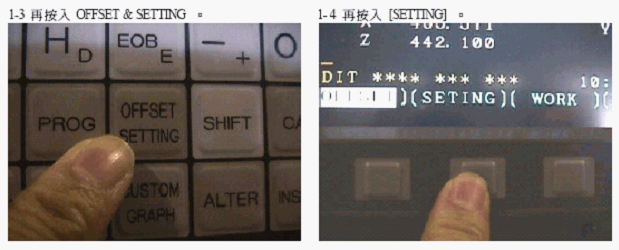
\includegraphics[width=0.8\textwidth]{images/14-8}
	%	\caption{格式化} \label{格式化}
\end{figure}

\begin{figure}[!hbtp]
	\centering	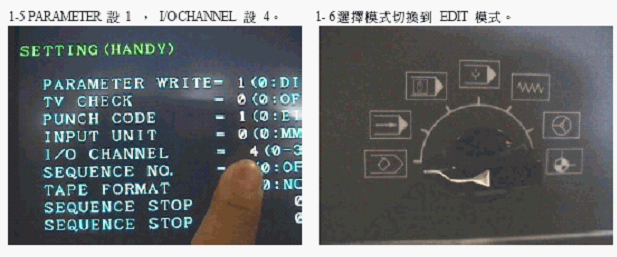
\includegraphics[width=0.8\textwidth]{images/14-9}
	%	\caption{格式化} \label{格式化}
\end{figure}


\begin{figure}[!hbtp]
	\centering	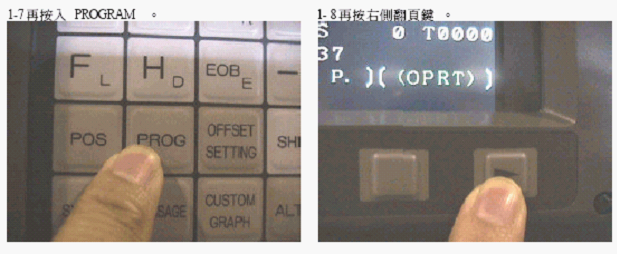
\includegraphics[width=0.8\textwidth]{images/14-10}
	%	\caption{格式化} \label{格式化}
\end{figure}

\begin{figure}[!hbtp]
	\centering	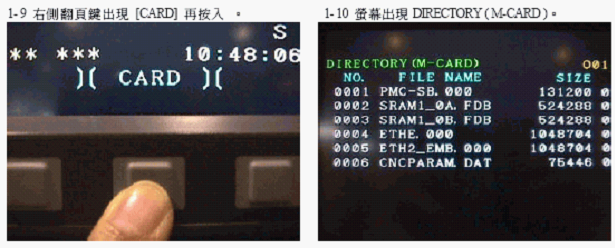
\includegraphics[width=0.8\textwidth]{images/14-11}
	\caption{读取程序操作步骤} \label{读取程序操作步骤}
\end{figure}

将NC记忆体的资料拷贝到(M-CARD)的步骤,如图\ref{NC到M-CARD}所示。

\begin{figure}[!hbtp]
	\centering	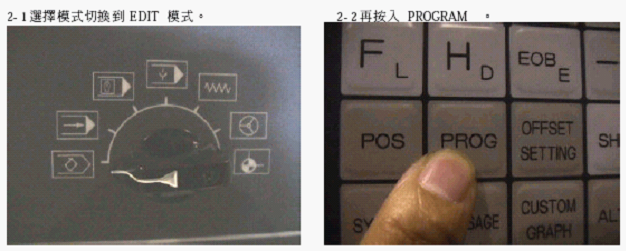
\includegraphics[width=0.8\textwidth]{images/14-12}
	%	\caption{格式化} \label{格式化}
\end{figure}

\begin{figure}[!hbtp]
	\centering	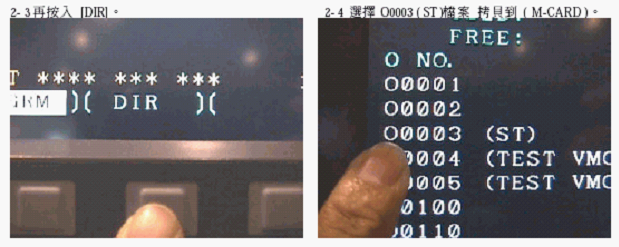
\includegraphics[width=0.8\textwidth]{images/14-13}
	%	\caption{格式化} \label{格式化}
\end{figure}

\begin{figure}[!hbtp]
	\centering	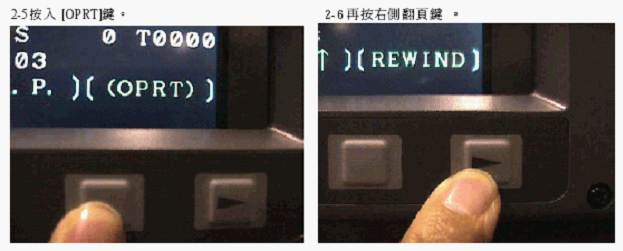
\includegraphics[width=0.8\textwidth]{images/14-14}
	%	\caption{格式化} \label{格式化}
\end{figure}

\begin{figure}[!hbtp]
	\centering	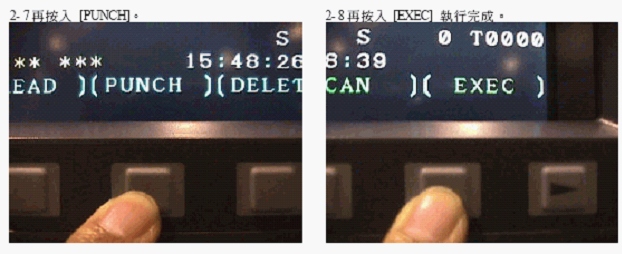
\includegraphics[width=0.8\textwidth]{images/14-15}
	%	\caption{格式化} \label{格式化}
\end{figure}

\begin{figure}[!hbtp]
	\centering	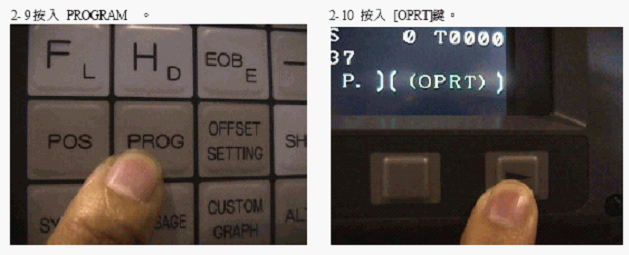
\includegraphics[width=0.8\textwidth]{images/14-16}
	%	\caption{格式化} \label{格式化}
\end{figure}

\begin{figure}[!hbtp]
	\centering	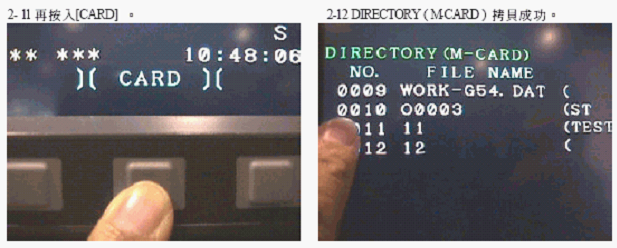
\includegraphics[width=0.8\textwidth]{images/14-17}
	\caption{NC到M-CARD} \label{NC到M-CARD}
\end{figure}

将(M-CARD)资料拷贝到NC记忆体的步骤,如图\ref{M-CARD到NC}所示。

\begin{figure}[!hbtp]
	\centering	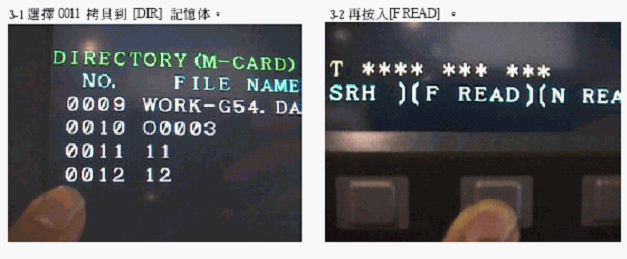
\includegraphics[width=0.8\textwidth]{images/14-18}
%	\caption{NC到M-CARD} \label{NC到M-CARD}
\end{figure}

\begin{figure}[!hbtp]
	\centering	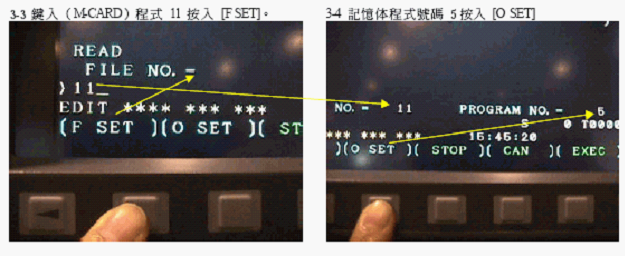
\includegraphics[width=0.8\textwidth]{images/14-19}
	%	\caption{NC到M-CARD} \label{NC到M-CARD}
\end{figure}

\begin{figure}[!hbtp]
	\centering	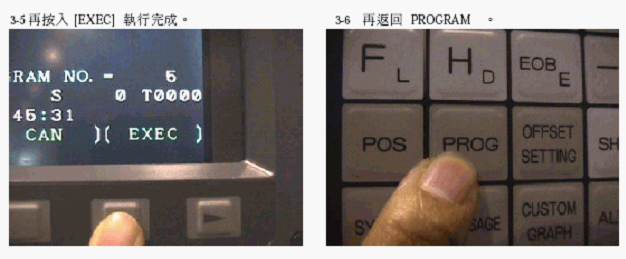
\includegraphics[width=0.8\textwidth]{images/14-20}
	%	\caption{NC到M-CARD} \label{NC到M-CARD}
\end{figure}

\begin{figure}[!hbtp]
	\centering	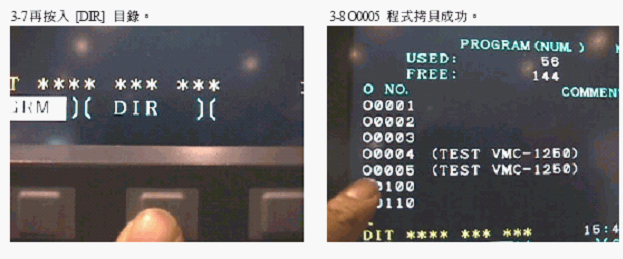
\includegraphics[width=0.8\textwidth]{images/14-21}
	\caption{M-CARD到NC} \label{M-CARD到NC}
\end{figure}

M-CARD程式刪除步骤,如图\ref{程式刪除}所示。

\begin{figure}[!hbtp]
	\centering	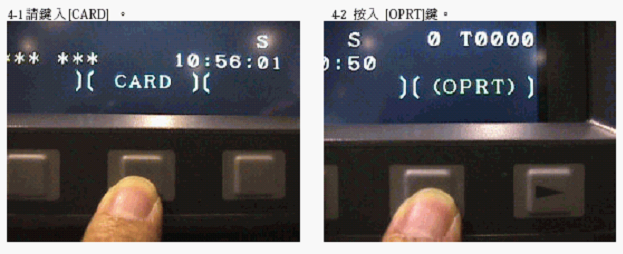
\includegraphics[width=0.8\textwidth]{images/14-22}
%	\caption{M-CARD到NC} \label{M-CARD到NC}
\end{figure}

\begin{figure}[!hbtp]
	\centering	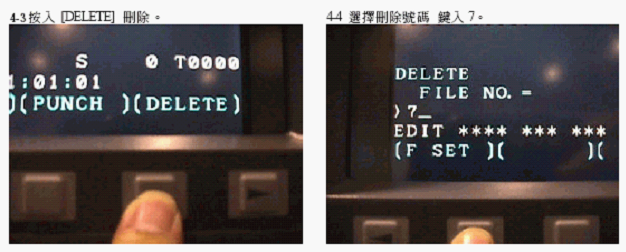
\includegraphics[width=0.8\textwidth]{images/14-23}
%	\caption{M-CARD到NC} \label{M-CARD到NC}
\end{figure}

\begin{figure}[!hbtp]
	\centering	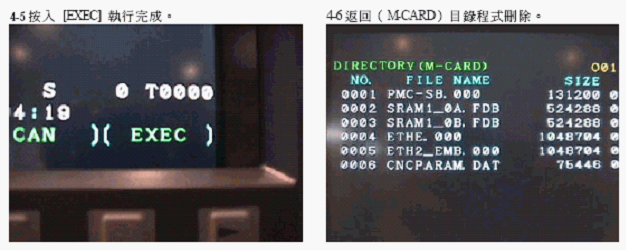
\includegraphics[width=0.8\textwidth]{images/14-24}
	\caption{程式刪除} \label{程式刪除}
\end{figure}
选择(M-CARD)DATA执行,如图\ref{M-CARD执行}所示。

\begin{figure}[!hbtp]
	\centering	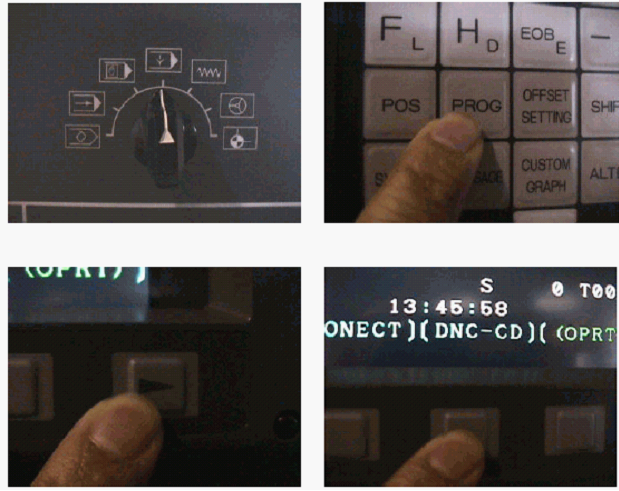
\includegraphics[width=0.8\textwidth]{images/14-25}
%	\caption{程式刪除} \label{程式刪除}
\end{figure}
\begin{figure}[!hbtp]
	\centering	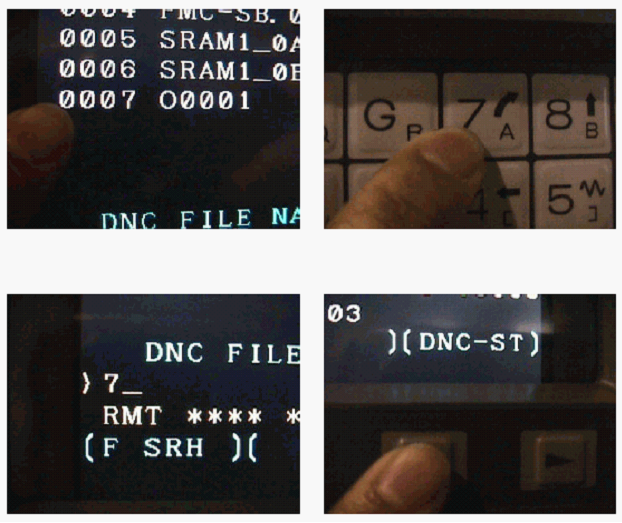
\includegraphics[width=0.8\textwidth]{images/14-26}
%	\caption{程式刪除} \label{程式刪除}
\end{figure}
\begin{figure}[!hbtp]
	\centering	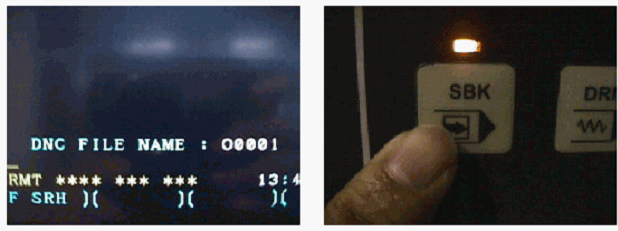
\includegraphics[width=0.8\textwidth]{images/14-27}
	\caption{M-CARD执行} \label{M-CARD执行}
\end{figure}

\newpage
\subsection{课堂小结}
\begin{enumerate}[1、]
	\item 数据线的接法;
	\item 传输过程;
	\item DNC 在线加工。
\end{enumerate}

\vfill
\subsection{布置作业}
\begin{enumerate}[1、]
	\item 写出上面的程序;
	\item 从习题集上选做一个。
\end{enumerate}
\vfill
\jxhj{%教学后记
	}
\skrq{%授课日期
	2017年5月30日 4-5节}
\ktmq{%课题名称
	 自动编程}
\jxmb{%教学目标,每行前面要加 \item
	\item 程序的传输;
	\item 程序的dnc加工;
	\item 自动编程刀路。}
\jxzd{%教学重点,每行前面要加 \item
	\item 程序的传输;
	\item 自动编程刀路。}
\jxnd{%教学难点,每行前面要加 \item
	\item 自动编程刀路。}
\jjff{%教学方法
	通过讲述、举例、演示法来说明;}

\makeshouye %制作教案首页

%%%%教学内容
\subsection{组织教学}
\begin{enumerate}[\hspace{2em}1、]
	\item 集中学生注意力;
	\item 清查学生人数;
	\item 维持课堂纪律;
\end{enumerate}
\subsection{复习导入及主要内容}
\begin{enumerate}[1、]
	\item 简单零件的倒角;
	\item 宏程序实例1;
	\item 宏程序实例2。
\end{enumerate}


\subsection{教学内容及过程}


\subsubsection{数据线的接法}
RS232通讯电缆

RS-232是美国电子工业联盟(EIA)制定的串行数据通信的接口标准,全称是EIA-RS-232(简称232,RS232)。它被广泛用于计算机串行接口外设连接。

RS-232C标准(协议),232是标识号,C代表RS232的最新一次修改(1969年),在这之前,还有RS232B、RS232A

FANUC机床25PIN    电脑 9PIN

Tx(02) ---------->---------- Rx(02)

Rx(03) ----------<---------- Tx(03)

GND(07) ------------------- GND(05)

RTS(04)-CD(08)------>------- CD(01)-CTS(08)

CTS(05) ----------<--------- DTR(04)

DSR(06)<-DTR(20)------>------ DSR(06)

屏蔽 ---------------------- 屏蔽

简化:(不能硬握手)

Tx(02) ----------->--------- Rx(02)

Rx(03) -----------<--------- Tx(03)

GND(07) ------------------- GND(05)

CD(08)-DSR(6)<-DTR(20)         CD(1)DTR(4)->DSR(6)

RTS(4)->CTS(5)                 RTS(7)->CTS(8)

屏蔽 ---------------------- 屏蔽

Siemens 9PIN      电脑9PIN  (只能使用硬握手)

Rx(02)--------<---------Tx(03)

Tx(03)-------->---------Rx(02)

DTR(04)------->---------DSR(06)

GND(05)-----------------GND(05)

DSR(06)-------<---------DTR(04)

RTS(07)-------->--------CTS(08)

CTS(08)--------<---------RTS(07)

Siemens 25PIN      电脑9PIN  (只能使用硬握手)

Rx(02)--------<---------Tx(03)

Tx(03)-------->---------Rx(02)

DTR(06)------->---------DSR(06)

GND(07)-----------------GND(05)

DSR(20)-------<---------DTR(04)

RTS(05)-------->--------CTS(08)

CTS(04)--------<---------RTS(07)

其中:

Tx 发送数据(发)          Rx接受数据(收)

DTR数据终端准备(发)     DSR数据准备好(收)

RTS请求发送          CTS清除发送

CD 数据载波检测

Tx、DTR和RTS信号是由数据终止设备(DTE)产生的,Rx、DSR、CTS、DCD信号是由数据通讯设备(DCE)产生的。

DCE(如打印机)-------DTE(如服务器)

连接两个DTE设备需要一个虚拟调制解调器来充当DCE,需交换相应的信号(TD-RD, DTR-DSR, and RTS-CTS),就是上面的接法。

握手是在通信电路建立之后,信息传输开始之前。 握手用于达成参数,如信息传输率,字母表,奇偶校验, 中断过程,和其他协议特性。

软件握手(XON/XOFF)------握手通过交换的打印机与通过在传输服务器之间的控制代码来实现的并分别接收行。 数据通讯设备的数据缓冲区满时它会发送通知服务器的打印处理器的 XOFF 暂停输出。 当缓冲区可用空间的更多的数据时发送一个 XON 字符,并且服务器将继续发送到下一个 XOFF。XON/XOFF可以工作于3线的接口

硬件握手(RTS/CTS) -----使用信号电压级别的信号进行控制,要求数据终端就绪 (DTR) 针 20 在打印机清除发送 (CTS) 针 5 和在服务器上的数据集就绪 (DSR) 6 针连接上。 当打印机数据缓冲区填充时,固定 20,DTR,电压级别从更改高为低。 这将指示服务器以停止发送数据。 当缓冲区可用空间的更多的数据时 DTR 电压级别切换高,并在服务器继续发送到下一个 DTR 电压拉。

相关参数:

•	波特率(又称鲍率): 是指从一设备发到另一设备的波特率,即每秒钟多少位元bits per second (bit/s)。典型的波特率是300, 1200, 2400, 9600, 115200, 19200等bit/s。一般通信两端设备都要设为相同的波特率,但有些设备也可以设置为自动检测波特率。

•	奇偶校验(Parity:是用来验证数据的正确性。奇偶校验一般不用,如果使用,那么既可以做奇校验(Odd Parity)也可以做偶校验(Even Parity)。奇偶校验是通过修改每一发送字节(也可以限制发送的字节)来工作的。如果不作奇偶校验,那么数据是不会被改变的。在偶校验中,因为奇偶校验位会被相应的置1或0(一般是最高位或最低位),所以数据会被改变以使得所有传送的数位(含字符的各数位和校验位)中“1”的个数为偶数;在奇校验中, 所有传送的数位(含字符的各数位和校验位)中“1”的个数为奇数。奇偶校验可以用于接受方检查传输是否发送生错误——如果某一字节中“1”的个数发生了错误,那么这个字节在传输中一定有错误发生。如果奇偶校验是正确的,那么要么没有发生错误要么发生了偶数个的错误。如果使用者选择资料长度为8位元,则因为没有多余的位元可被用来作为同位元,因此就叫做“无位元(Non Parity)”。

•	停止位:是在每个字节传输之后发送的,它用来帮助接受信号方硬件重同步,即把同步讯号与资料混和之后,使用同一条传输线来传输。比如资料11001010被传输时,资料的前后就需加入Start(Low)以及Stop(High)等两个位元,Start讯号固定为一个位元,但Stop停止位元则可以是1、1.5或者是2位元。

\subsubsection{传输过程}
设定好两边的参数:

Siemens 参数      Fanuc 参数

PC 参数

传输程序:

Fanuc:

Siemens

\%\_N\_name\_MPF    或\%\_N\_name\_SPF

;PATH=/\_DIR\_MPF

\subsubsection{DNC 在线加工}

Fanuc存储卡的使用

(一).CF卡初期格式化步骤:

1将NC的I/O频道设定为4,设定页面按【setting】进入,如图\ref{频道设定}所示:

\begin{figure}[!hbtp]
	\centering	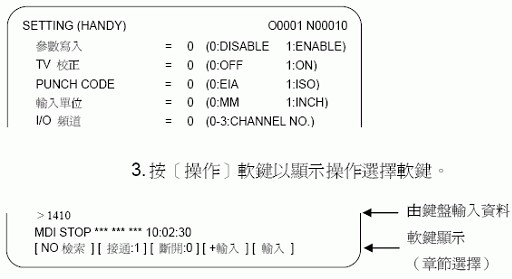
\includegraphics[width=0.9\textwidth]{images/14-1}
	\caption{频道设定} \label{频道设定}
\end{figure}

2关闭CNC系统及机台总电源;

3打开机台电控箱,将安装好的PCMCIA接口的CF卡插入到FANUC 0i主机的【CNMC】插槽,安装时注意方向,不可用力过猛;
如图\ref{插入PCMCIA卡}所示。

\begin{figure}[!hbtp]
	\centering	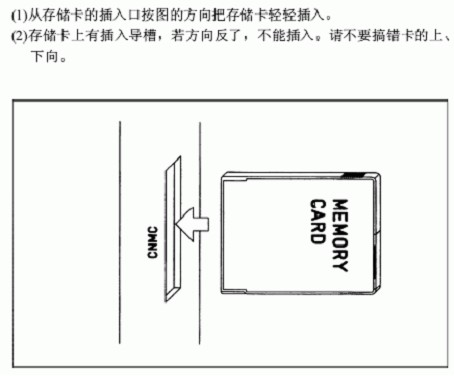
\includegraphics[width=0.9\textwidth]{images/14-2}
	\caption{插入PCMCIA卡} \label{插入PCMCIA卡}
\end{figure}

4进入NC的BOOT界面,方法为:同时按住屏幕下方最右边的两个软建,如图\ref{进入BOOT界面}所示:

\begin{figure}[!hbtp]
\centering	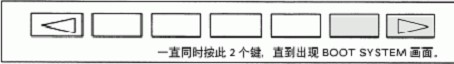
\includegraphics[width=0.9\textwidth]{images/14-3}
\caption{进入BOOT界面1} \label{进入BOOT界面}
\end{figure}

同时开启NC电源,直到出现如图\ref{进入BOOT界面1}的画面:

\begin{figure}[!hbtp]
\centering	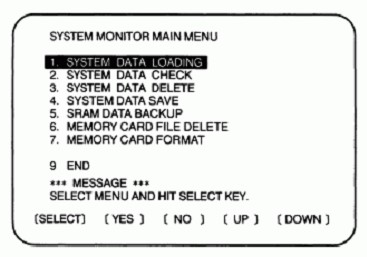
\includegraphics[width=0.9\textwidth]{images/14-4}
\centering	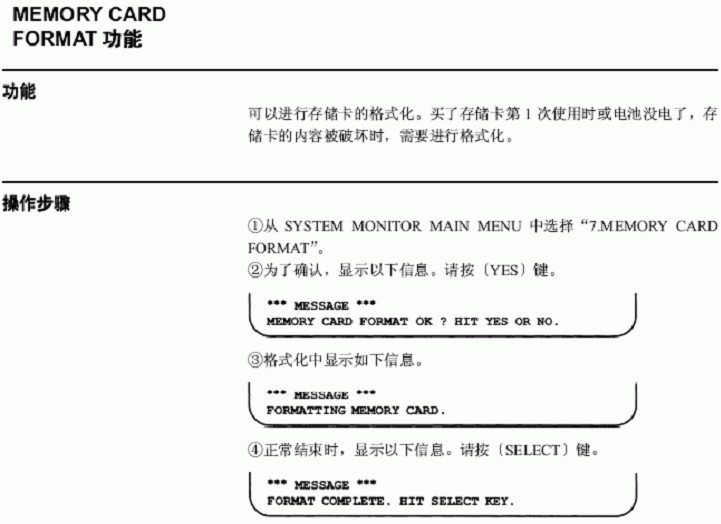
\includegraphics[width=0.9\textwidth]{images/14-5}
\caption{进入BOOT界面2} \label{进入BOOT界面1}
\end{figure}

格式化完成后,退出BOOT界面,重启系统,退出步骤如图\ref{格式化}所示:
\begin{figure}[!hbtp]
	\centering	\includegraphics[width=0.9\textwidth]{images/14-6}
	\caption{格式化} \label{格式化}
\end{figure}

如果一切正常,格式过的CF卡,就可以在FANUC0i系统中使用了。如程式的存储,备份,调用等。

(二).PCMCIA卡在FANUC0i系统上的使用

Oi-MB PCMCIA读取程序操作步骤,如图\ref{读取程序操作步骤}所示。
\begin{figure}[!hbtp]
	\centering	\includegraphics[width=0.8\textwidth]{images/14-7}
%	\caption{格式化} \label{格式化}
\end{figure}

\begin{figure}[!hbtp]
	\centering	\includegraphics[width=0.8\textwidth]{images/14-8}
	%	\caption{格式化} \label{格式化}
\end{figure}

\begin{figure}[!hbtp]
	\centering	\includegraphics[width=0.8\textwidth]{images/14-9}
	%	\caption{格式化} \label{格式化}
\end{figure}


\begin{figure}[!hbtp]
	\centering	\includegraphics[width=0.8\textwidth]{images/14-10}
	%	\caption{格式化} \label{格式化}
\end{figure}

\begin{figure}[!hbtp]
	\centering	\includegraphics[width=0.8\textwidth]{images/14-11}
	\caption{读取程序操作步骤} \label{读取程序操作步骤}
\end{figure}

将NC记忆体的资料拷贝到(M-CARD)的步骤,如图\ref{NC到M-CARD}所示。

\begin{figure}[!hbtp]
	\centering	\includegraphics[width=0.8\textwidth]{images/14-12}
	%	\caption{格式化} \label{格式化}
\end{figure}

\begin{figure}[!hbtp]
	\centering	\includegraphics[width=0.8\textwidth]{images/14-13}
	%	\caption{格式化} \label{格式化}
\end{figure}

\begin{figure}[!hbtp]
	\centering	\includegraphics[width=0.8\textwidth]{images/14-14}
	%	\caption{格式化} \label{格式化}
\end{figure}

\begin{figure}[!hbtp]
	\centering	\includegraphics[width=0.8\textwidth]{images/14-15}
	%	\caption{格式化} \label{格式化}
\end{figure}

\begin{figure}[!hbtp]
	\centering	\includegraphics[width=0.8\textwidth]{images/14-16}
	%	\caption{格式化} \label{格式化}
\end{figure}

\begin{figure}[!hbtp]
	\centering	\includegraphics[width=0.8\textwidth]{images/14-17}
	\caption{NC到M-CARD} \label{NC到M-CARD}
\end{figure}

将(M-CARD)资料拷贝到NC记忆体的步骤,如图\ref{M-CARD到NC}所示。

\begin{figure}[!hbtp]
	\centering	\includegraphics[width=0.8\textwidth]{images/14-18}
%	\caption{NC到M-CARD} \label{NC到M-CARD}
\end{figure}

\begin{figure}[!hbtp]
	\centering	\includegraphics[width=0.8\textwidth]{images/14-19}
	%	\caption{NC到M-CARD} \label{NC到M-CARD}
\end{figure}

\begin{figure}[!hbtp]
	\centering	\includegraphics[width=0.8\textwidth]{images/14-20}
	%	\caption{NC到M-CARD} \label{NC到M-CARD}
\end{figure}

\begin{figure}[!hbtp]
	\centering	\includegraphics[width=0.8\textwidth]{images/14-21}
	\caption{M-CARD到NC} \label{M-CARD到NC}
\end{figure}

M-CARD程式刪除步骤,如图\ref{程式刪除}所示。

\begin{figure}[!hbtp]
	\centering	\includegraphics[width=0.8\textwidth]{images/14-22}
%	\caption{M-CARD到NC} \label{M-CARD到NC}
\end{figure}

\begin{figure}[!hbtp]
	\centering	\includegraphics[width=0.8\textwidth]{images/14-23}
%	\caption{M-CARD到NC} \label{M-CARD到NC}
\end{figure}

\begin{figure}[!hbtp]
	\centering	\includegraphics[width=0.8\textwidth]{images/14-24}
	\caption{程式刪除} \label{程式刪除}
\end{figure}
选择(M-CARD)DATA执行,如图\ref{M-CARD执行}所示。

\begin{figure}[!hbtp]
	\centering	\includegraphics[width=0.8\textwidth]{images/14-25}
%	\caption{程式刪除} \label{程式刪除}
\end{figure}
\begin{figure}[!hbtp]
	\centering	\includegraphics[width=0.8\textwidth]{images/14-26}
%	\caption{程式刪除} \label{程式刪除}
\end{figure}
\begin{figure}[!hbtp]
	\centering	\includegraphics[width=0.8\textwidth]{images/14-27}
	\caption{M-CARD执行} \label{M-CARD执行}
\end{figure}

\newpage
\subsection{课堂小结}
\begin{enumerate}[1、]
	\item 数据线的接法;
	\item 传输过程;
	\item DNC 在线加工。
\end{enumerate}

\vfill
\subsection{布置作业}
\begin{enumerate}[1、]
	\item 写出上面的程序;
	\item 从习题集上选做一个。
\end{enumerate}
\vfill
\jxhj{%教学后记
	}
\skrq{%授课日期
	2017年6月6日 4-5节}
\ktmq{%课题名称
	 复习}
\jxmb{%教学目标,每行前面要加 \item
	\item 复习相关知识;
	\item 巩固相关知识。}
\jxzd{%教学重点,每行前面要加 \item
	\item 复习相关知识;
	\item 巩固相关知识。}
\jxnd{%教学难点,每行前面要加 \item
	\item 巩固相关知识。}
\jjff{%教学方法
	通过讲述、举例、演示法来说明;}

\makeshouye %制作教案首页

%%%%教学内容
\subsection{组织教学}
\begin{enumerate}[\hspace{2em}1、]
	\item 集中学生注意力;
	\item 清查学生人数;
	\item 维持课堂纪律;
\end{enumerate}
\subsection{复习导入及主要内容}
\begin{enumerate}[1、]
	\item 绘制图形;
	\item 面铣加工;
	\item 外形加工。
\end{enumerate}


\subsection{教学内容及过程}
\subsubsection{小结}
本学期教学工作上的总结,学生学习上的总结,学生作业完成上的总结,学生实习操作上的总结,学生实习报告上的总结,及总体评介,肯定其优点,并指出不足。
\subsubsection{期终考试相关知识}
选择、判断、填空、问答、编程、作图、改错。
\subsubsection{复习基本指令}
G指令\par
G0 G1 G2 G3\par
G17 G18 G19\par
G9 G61 G62 G63 G64\par
G4 \par
G20 G21\par
G40 G41 G42 \par
G43 G44 G49\par
G90 G91\par
G98 G99\par
G81 G82 G83 G84 G85 G86 G87 G88 G89 G80 G73 G74 G76\par
M指令\par
M0 M1 M2 M30\par
M3 M4 M5 M19\par
M6 M7 M8 M9\par
M98 M99\par
其它指令\par
\subsubsection{复习相关知识}
数控加工工艺学\par
数学知识\par
刀具、量具的选择及使用\par
热处理、\par
计算机知识\par
CAD/CAM\par
\subsubsection{复习机床操作知识}\par
操作方式:回零、手动、手轮、MDI、自动、快速、编辑\par
开机\par
手动回参考点\par
手动返回\par
输入程序\par
参数设定\par
程序检查及测试\par
自动加工\par
测量\par
安全:\par
\subsubsection{复习编程思路}
平面\par
外轮廓\par
挖槽(岛屿)\par
孔、\par
凸轮槽\par
薄壁\par
复杂零件\par
配合零件\par
CAD/CAM\par
宏程序\par

\subsection{课堂小结}
\begin{enumerate}[1、]
	\item 小结;
	\item 基本指令;
	\item 相关知识
	\item 机床操作
	\item 编程思路。
\end{enumerate}

\vfill
\subsection{布置作业}
\begin{enumerate}[1、]
	\item 自我复习。
\end{enumerate}
\vfill


\biaoti{实习}%标题头
\setcounter{section}{0}%重新计数
%重新设定目录
%\titlecontents{section}[0pt]{\addvspace{5pt}\filright}
%{ 实习  \thecontentslabel \hspace{0.5em} }
%{}{\titlerule*[8pt]{.} \contentspage}
%\jxhj{%教学后记
	大部分同学能够回忆起所学的知识,达到教学效果。}
\skrq{%授课日期
	}
\ktmq{%课题名称
	复习上期所学内容 }
\jxmb{%教学目标,每行前面要加 \item
	\item 巩固上期的基本指令;

	\item 总结上期的编程思路;

	\item 总结机床的操作技巧;

	\item 了解本期的学习内容及学生情况;}
\jxzd{%教学重点,每行前面要加 \item
	\item 巩固上期的基本指令;
	\item 总结上期的编程思路;}
\jxnd{%教学难点,每行前面要加 \item
	\item 总结上期的编程思路;}
\jjff{%教学方法
	通过讲述、举例、演示法来说明;}

\makeshouye %制作教案首页

%%%%教学内容
\subsection{组织教学}
\begin{enumerate}[\hspace{2em}1、]
	\setlength{\itemsep}{0pt}
	\item 集中学生注意力;
	\item 清查学生人数;
	\item 维持课堂纪律;
\end{enumerate}
\subsection{复习导入及主要内容}
\begin{enumerate}[\hspace{2em}1、]
	\item 上学期末考试讲评;

	\item 了解学生情况;
\end{enumerate}
\subsection{教学内容及过程}
\subsubsection{本期教学安排} \marginpar{说明介绍}
\paragraph{理论教学计划:}
\begin{itemize}
	\item 复习导入

	\item 变量编程概述

	\item 变量Z向分层

	\item 椭圆编程

	\item 椭圆弧编程

	\item 局部坐标系

	\item 坐标系旋转(一)

	\item 坐标系旋转(二)

	\item 极坐标指令

	\item 期中测试

	\item 试卷讲解

	\item 孔系变量编程

	\item 变量周边导圆角

	\item 自动编程
	\item 综合练习

	\item 期末复习
\end{itemize}

\paragraph{实习教学计划}
\begin{itemize}
	\item 六面四方体加工

	\item 六面圆槽加工

	\item 椭圆加工

	\item 薄壁配合加工
\end{itemize}

\subsubsection{手工编程复习} \marginpar{互动提问}
如下面的思维导图 \ref{手工编程思维导图}
\begin{figure}	
	\includegraphics{images/tu1} 
	\caption{手工编程思维导图}\label{手工编程思维导图}
\end{figure}

\subsubsection{数控机床的操作}
如下面的思维导图 \ref{数控机床的操作思维导}
\begin{figure}	
	\includegraphics{images/tu2} 
	\caption{数控机床的操作思维导图} \label{数控机床的操作思维导}
\end{figure}

\subsubsection{数控机床指令}
\paragraph{G指令}\begin{itemize}
	\item G0 G1 G2 G3

	\item G17 G18 G19

	\item G9 G61 G62 G63 G64

	\item G4 \marginpar{说明介绍说明介绍说明介绍说明介绍说明介绍说明介绍}

	\item G20 G21

	\item G40 G41 G42 

	\item G43 G44 G49 \marginpar{说明介绍说明介绍说明介绍说明介绍说明介绍说明介绍}

	\item G90 G91

	\item G98 G99

	\item G81 G82 G83 G84 G85 G86 G87 G88 G89 G80 G73 G74 G76

\end{itemize}

\paragraph{M指令}

\begin{itemize}
	\item M0 M1 M2 M30

	\item M3 M4 M5 M19 

	\item M6 M7 M8 M9

	\item M98 M99

\end{itemize}

\paragraph{其它指令}
\subsubsection{常见加工结构}
\begin{itemize}
	\item 平面

	\item 外轮廓

	\item (岛屿)

	\item 孔
	\item 凸轮槽

	\item 复杂零件

	\item 配合零件

	\item CAD/CAM

	\item 宏程序

	\item 其它
\end{itemize}
\subsubsection{上学期期末试卷分析}
\subsection{课堂小结}
主要复习了数控方面的基本知识。
\vfill
\subsection{布置作业}
\begin{enumerate}[1、]
	\item 自选一零件图, 写出其工艺与程序;

	\item 写出如图所示零件的程序及与工艺;
\end{enumerate}
\vfill

%\jxhj{%教学后记
	}
\skrq{%授课日期
	2017年2月27日 4-5节}
\ktmq{%课题名称
	变量编程概述 }
\jxmb{%教学目标,每行前面要加 \item
	\item 掌握变量的概念;

	\item 掌握变量的赋值于引用;

	\item 掌握表达式的使用;

	\item 会用变量编程;}
\jxzd{%教学重点,每行前面要加 \item
	\item 变量的概念;

	\item 表达式的使用;}
\jxnd{%教学难点,每行前面要加 \item
	\item 用变量编程;}
\jjff{%教学方法
	通过讲述、举例、演示法来说明;}

\makeshouye %制作教案首页

%%%%教学内容
\subsection{组织教学}
\begin{enumerate}[\hspace{2em}1、]
	\item 集中学生注意力;
	\item 清查学生人数;
	\item 维持课堂纪律;
\end{enumerate}
\subsection{复习导入及主要内容}
\begin{enumerate}[\hspace{2em}1、]
\item 复习;
\item 了解学生情况;
\end{enumerate}
\subsection{教学内容及过程}
\subsubsection{变量与常量} \marginpar{举例说明}
常量:指其值不变的量。如数值:1、4、6
\par
字符: “A”、“b”
\par
布尔值:“TURE”、“FALSE”
\par
变量:由变量名(变量号)和变量值组成,其值可以改变,

变量就是指其值可以改变的量。
\par
分析:程序结构相同,如果使用变量,则两个程序可以合为一个程序。
\par
长 宽 圆弧半径 深度等 都可以使用变量

可以用表达式来指定变量。
\subsubsection{Fanuc上的变量}
\begin{enumerate}[1、]
	\item 变量号(变量名)


\#1-\#33 

  \#100-\#199 
  
   \#500-\#999  
   
   \#1000以上


由变量符号“\#”和后面的变量号组成。
\item 变量的赋值:


赋值是指将一个数据赋予一个变量
\begin{enumerate}[(1)]
	\item 在程序中赋值:

\#1=10      \#2=5+5       \#3=\#3+1  \#5=\#7


注意: “=”为赋值号, 并等于号


赋值号“=”两内容不能随意互换, 左边只能是变量, 而右边可有是表达式, 数值或变量.


一个赋值语句只能给一个变量赋值.


可以多次给一个变量赋值, 新变量值将取代原变量值. 


赋值表达式的运算顺序与数学运算顺序相同


\item 在宏程序调用指令中赋值:(不讲)


如 G66 P5000 A10.0 B11.0


A10.0 B11.0 会给5000号宏程序中的\#1, \#2 赋值


宏调用中的A B C 与 \#1 \#2… \#20有一种邦定关系.


\item  在系统参数中设定变量的值:


Fanuc中操作如下: 


Offset-----[下一页]-------[Macro]


\#1--\#33   \#100--\#199   \#500--\#999


\end{enumerate}

\item 变量值的范围及小数点


定义变量时,整数值的小数点可以省略。

如:\# 100=123   变量\#100的值为123.000

\item 变量值的引用

在程序中使用变量时, 在相应的字后跟上变量号即可. 当用表达式指定变量时, 必须把表达式放在括号中, 如
:

G1 X\#\ 1 Y\#2


G1 X[-\#1-10] 


改变变量的符号, 可直接在\#前面加“-”, 如 G1 X-\#1


注意: O N G L P / 后不能使用变量.


程序的修改。
\end{enumerate}

\subsubsection{变量的分类} 
系统变量, 用于系统内部运算时各种数据的存储. \#1000以上,如刀具当前位置和补偿值等.


用户变量, 包括局部变量与公共变量, 用户可以单独使用, 系统作为处理资料的一部分.


局部变量: \#1-\#33 , 只能在宏程序中存储数据, 例如运算结果, 断电时,局部变量清除(初始值为空)


公共变量: \#100-\#199(数据断电清除)


\#500-\#999(数据断电时也不会清除)


公共变量在不同的宏程序中意义相同(即公共变量对于主程序和从这些主程序调用的每一个宏程序来说是公用的.)


举例说明:  个人的钱包   局部的


班上的班费   公共的


实例程序的修改:讲解

\subsubsection{算术} 

1. 加减乘除:
\\
\#i=\#j+\#k           \#i=\#j-\#k
\\
\#i=\#j*\#k           \#i=\#j/\#k
 \\
2.三角函数:
\\
\#i=SIN[\#j]          \#i=COS[\#j]
\\
\#i=ASIN[\#j]         \#i=ACOS[\#j]
\\
\#i=TAN[\#j]         \#i=ATAN[\#j]/[\#k] (可理解为对边/邻边)
\\
注意: 三角函数及反三角函数的数值均以度为单位来指定
\\
如90度30分应表示为90.5度
\\
3.开平方根,舍入,绝对值:
\\
\#i=SQRT[\#j]        \#i=ABS[\#j]
\\
\#i=ROUND[\#j]
\\
4.指数对数
\\
\#i=EXP[\#j]
\\
\#i=LN[\#j]
\\
5.取整
\\
上取整  \#i=FIX[\#j]
\\
下取整  \#i=FUP[\#j]
\subsubsection{运算顺序与括号}
\subsection{课堂小结}
\vfill
\subsection{布置作业}
\begin{enumerate}[1、]
	\item 自选一零件图, 写出其工艺与程序.
	\item 写出如图所示零件的程序及与工艺.
\end{enumerate}
\vfill


%% 中文习惯是设定首行缩进为2em。注意此设置一定要在document环境之中,这可能与\setlength作用范围相关
%\setlength{\parindent}{2em}                    
%
%\title{Xecjk Template Test}
%\author{Xiao Hanyu}
%\maketitle
%
%\tableofcontents
%\listoffigures
%%\listoftablescontent
%
%\section{基本文字测试}
\label{sec:1}
我叫肖晗宇,来自浙江大学计算机学院,热爱开源软件、旅行、摄影,推崇互助共享的精神理念。

My name is Xiao Hanyu, a student from Computer Science and Technology of Zhejiang University, I love open source software, travelling all over the world, photography, and so on. 

我喜欢\LaTeXe,也推荐大家来学习使用\LaTeXe,以下是比较不错的学习资源:

\begin{enumerate}
\item LaTeX companion
\item The TeXbook
\end{enumerate}


\section{图形图像测试}
\subsection{插图测试}
Hand in Hand:\ref{fig:hand_in_hand}
\begin{figure}[htbp]
\centerline{\includegraphics[width=0.6\textwidth]{images/hand_in_hand.png}}
\caption[]{\label{fig:hand_in_hand} 手拉手}
\end{figure}

\subsection{pgf/tikz绘图测试}
图\ref{fig:monotonic_chain}是用pgf/tikz宏包作的图形,用以说明计算几何相关定理。

\begin{figure}
\centering
\begin{tikzpicture}[line width=2pt]
\draw (-1,0) -- (8,0);
\draw (0,-1) -- (0,8);
\draw[step=.5cm, very thin] (0,0) grid (7.2,7.2);

\coordinate [label=above:$A$] (A) at (1, 4);
\coordinate [label=left:$B$] (B) at (0.5, 3.5);
\coordinate [label=left:$C$] (C) at (1, 3);
\coordinate [label=left:$D$] (D) at (0.3, 1.3);
\coordinate [label=below:$E$] (E) at (1, 1);

\draw[blue] (A) -- (B) -- (C)  -- (D) -- (E);
\draw[blue] (2, 0) -- (2, 6);

\coordinate [label=right:$A'$] (A') at (2, 4);
\coordinate [label=right:$B'$] (B') at (2, 3.5);
\coordinate [label=right:$C'$] (C') at (2, 3);
\coordinate [label=right:$D'$] (D') at (2, 1.3);
\coordinate [label=right:$E'$] (E') at (2, 1);

\draw[blue] (A) -- (A');
\draw[blue] (B) -- (B');
\draw[blue] (C) -- (C');
\draw[blue] (D) -- (D');
\draw[blue] (E) -- (E');

\coordinate [label=above:$a$] (a) at (5, 4);
\coordinate [label=left:$b$] (b) at (4.5, 4.5);
\coordinate [label=left:$c$] (c) at (5, 3);
\coordinate [label=left:$d$] (d) at (4.3, 1.3);
\coordinate [label=below:$e$] (e) at (5, 1.3);

\draw[green] (a) -- (b) -- (c)  -- (d) -- (e);
\draw[green] (6, 0) -- (6, 6);

\coordinate [label=right:$a'$] (a') at (6, 4);
\coordinate [label=right:$b'$] (b') at (6, 4.5);
\coordinate [label=right:$c'$] (c') at (6, 3);
\coordinate [label=right:$d'$] (d') at (6, 1.3);
\coordinate [label=right:$e'$] (e') at (6, 1.3);

\draw[green] (a) -- (a');
\draw[green] (b) -- (b');
\draw[green] (c) -- (c');
\draw[green] (d) -- (d');
\draw[green] (e) -- (e');
\end{tikzpicture}
\caption{Monotonic polygonal chains}
\label{fig:monotonic_chain}
\end{figure}

\section{表格测试}
\begin{table}[htbp]
  \centering
  \begin{tabular}[htbp]{r|l}
    \toprule
    日期 & 任务 \\
    \midrule
    2011.5 & 完善此份文档 \\
    2011.6 & 完善安装脚本 \\
    \bottomrule
  \end{tabular}
  \caption{表格}
  \label{tab:table1}
\end{table}

\section{源代码高亮测试}

以下是\href{http://acm.zju.edu.cn/onlinejudge/showProblem.do?problemCode=1372}{ZOJ 1372}的解题c++代码:

\begin{lstlisting}[language=c++]
#include <iostream>
#include <string>
using namespace std;
 
const long max_points = 100;
const long infinity = 1000001;
 
int p, r, length, g[max_points][max_points];
bool flag;
 
class vertex
{
public:
    int distance;
    bool visited;
};
 
vertex v[max_points];
 
void initial()
{
    for(int i = 1; i <= p; i++)
        for(int j = 1; j <= p; j++)
            g[i][j] = infinity;
}
 
void prim(int origin)
{
    int temp_min;
    int temp_v = 0;
    int sum = 0;
 
    for(int i = 1; i <= p; i++)
    {
        v[i].distance = g[i][origin];
        v[i].visited = false;
    }
 
    v[origin].distance = 0;
    v[origin].visited = true;
 
    sum++;
 
    while (sum < p)
    {
        temp_min = infinity;
        for(int i = 1; i <= p; i++)
            if(v[i].visited == false && v[i].distance < temp_min)
            {
                temp_min = v[i].distance;
                temp_v = i;
            }
         
        if(temp_min < infinity)
        {
            length += v[temp_v].distance;
            v[temp_v].visited = true;
            sum++;
        }
        else
        {
            flag = true;
            break;
        }
 
        for(int i = 1; i <= p; i++)
        {
            if(v[i].visited == false && v[i].distance > g[i][temp_v])
            {
                v[i].distance = g[i][temp_v];
            }
        }
    }
}
 
int main(int argc, char *argv[])
{
    int a, b, c;
 
    while(cin >> p)
    {
        if(p == 0)
            break;
        cin >> r;
 
        initial();
 
        for(int i = 0; i < r; i++)
        {
            cin >> a >> b >> c;
            if(c < g[a][b])
                g[a][b] = g[b][a] = c;
        }
        length = 0;
        prim(1);
 
        cout << length << endl;
    }
 
    return 0;
} 
\end{lstlisting}

\section{数学公式测试}

著名的爱因斯坦质能方程(\ref{eq:emc2}):

\begin{equation}
  \label{eq:emc2}
  E=mc^2
\end{equation}

计算$f(x)=x^2$的不定积分(\ref{eq:2}):

\begin{equation}
  \label{eq:2}
  \int x^2 dx = \frac{1}{3} x^3
\end{equation}
\section{参考文件测试}
参考文件最好使用bibtex,关于bibtex的使用方法,你可以自行查阅相关文献。

这里是参考文献\cite{c_minigui}

%%%%%%%%%------------------------------------------------------------------------
%%%% 附录

% \appendix    
% \appendixpage
%% 将附录条目添加到contents
% \addappheadtotoc

%%%% 附录结束
%%%%%%%%------------------------------------------------------------------------

%
%%% 加入参考文献支持
%\bibliography{data/main}
%%% 解决目录中没有相应的参考文献的条目问题
%\addcontentsline{toc}{section}{\refname} 
\end{document}
%%%% 正文部分结束
%%%%%%%%------------------------------------------------------------------------
